\documentclass[aps,prb,twocolumn,superscriptaddress,floatfix]{revtex4-2}

\usepackage[T1]{fontenc}
\usepackage{amsmath,amssymb,bm}
\usepackage{graphicx}
\usepackage{booktabs}
\usepackage{xcolor}
\usepackage{microtype}
\usepackage[hidelinks]{hyperref}

\graphicspath{{figures/}}

\newcommand{\Tmf}{T_{\mathrm{MF}}}
\newcommand{\rlead}{\rho_{\mathrm{lead}}}
\newcommand{\Jb}{\bar{J}}
\newcommand{\Tr}{\operatorname{Tr}}

\begin{document}

\title{Thermal Phase Fluctuations, Vortex Pinning, and the Hierarchy of Superconducting Coherence on Fractal Lattices}

\author{Robert Canyellas}
\affiliation{Institute for Molecules and Materials, Radboud University, Heyendaalseweg 135, 6525AJ Nijmegen, The Netherlands}

\author{Mikhail I. Katsnelson}
\affiliation{Institute for Molecules and Materials, Radboud University, Heyendaalseweg 135, 6525AJ Nijmegen, The Netherlands}

\author{Andrey A. Bagrov}
\affiliation{Institute for Molecules and Materials, Radboud University, Heyendaalseweg 135, 6525AJ Nijmegen, The Netherlands}

\date{\today}

\begin{abstract}
Mean-field Bogoliubov--de Gennes (BdG) theory predicts that finitely ramified fractal geometries can strongly amplify the superconducting pairing gap and the pair-formation temperature $\Tmf$ relative to their regular parent lattices. In low dimensions, however, the true superconducting transition is governed not by local pair formation, but by the resilience of macroscopic phase coherence against thermal fluctuations and vortex proliferation. Here we investigate how thermal phase and amplitude fluctuations control superconducting coherence on finite fractal flakes---the infinitely ramified Sierpi\'nski carpet and the finitely ramified triangular and honeycomb Sierpi\'nski gaskets---by constructing a four-rung hierarchy of microscopic approximations within the attractive Hubbard model. Sharing identical two-terminal lead geometries and conductance normalization across all rungs, we compare (A)~the exact self-consistent BdG two-terminal phase stiffness without thermal fluctuations, (B)~Monte Carlo simulations of an effective nearest-neighbor classical XY model with temperature-dependent BdG bond couplings $J_b(T)$, (P)~frozen-amplitude fermionic BdG Hybrid Monte Carlo (HMC) sampling the exact nonlocal quasiparticle determinant, and (C)~full static-path BdG HMC sampling both pairing amplitudes and phases. We first establish the baseline thermodynamics of the uniform nearest-neighbor XY model across up to seven fractal generations, demonstrating that fractal lacunae induce a scale-separated hierarchy of vortex activation in which large holes populate with topological charge far below the onset of microscopic plaquette vortices. On the finitely ramified gaskets, the finite-size coherence crossover drifts algebraically toward zero with linear size, $T^*(G) \propto L^{-x}$ ($x \simeq 0.50$--$0.56$), whereas the infinitely ramified carpet exhibits a much slower drift ($x \simeq 0.15$) and a persistent fourth-order helicity dip characteristic of collective Berezinskii--Kosterlitz--Thouless (BKT) unbinding. In the microscopic fermionic problem, we show that weak-coupling gaskets open a wide pseudogap regime of incoherent Cooper pairs: despite an enhanced $\Tmf$, thermal fluctuations suppress the phase-coherence crossover severalfold below that of the filled parent lattice. Because the gasket coherence length collapses to the lattice scale, the local XY mapping (Rung~B) reproduces the exact fermionic HMC crossover (Rungs~P and~C) to within roughly $15\%$ on the gaskets, whereas on filled lattices and carpets Pippard nonlocality and anharmonic phase gradients reduce the fermionic HMC crossover well below the XY prediction. Finally, minimum-energy escape-path calculations on the full BdG free-energy landscape reveal that while fractal lacunae act as deep vortex traps in a phase-only XY description, local suppression of the pairing amplitude at corner bottlenecks lowers vortex escape barriers by an order of magnitude, preventing long-lived metastable vortex pinning on dc transport timescales.
\end{abstract}

\maketitle

%======================================================================
\section{Introduction}
\label{sec:intro}
%======================================================================

Quantum dynamics on artificial fractal lattices has recently evolved from a mathematical abstraction into an experimentally accessible frontier of condensed matter physics. Advances in scanning tunneling microscopy (STM) manipulation of CO molecules on Cu(111)~\cite{Kempkes2019}, surface-assisted molecular self-assembly~\cite{Shang2015}, and epitaxial growth of bismuth nanostructures~\cite{Canyellas2024Bi} now enable the atom-by-atom fabrication of deterministic fractal arrays with tailored Hausdorff dimension and ramification topology. In the superconducting regime, mesoscopic realizations have an even longer pedigree: lithographically patterned wire networks and Josephson-junction arrays arranged as Sierpi\'nski gaskets have been probed via magnetoresistance and two-coil mutual inductance since the late 1980s~\cite{Gordon1986,Meyer1991,Meyer2002,Amundsen2024}. From a theoretical perspective, fractal geometries occupy a unique niche between regular integer-dimensional crystals and randomly disordered media~\cite{Mandelbrot1982,Akkermans2012}. Their discrete scale invariance and non-integer Hausdorff dimension reshape single-particle spectra~\cite{Domany1983,Rammal1984}, quantum transport~\cite{Iliasov2020,Westerhout2018}, and topological edge or corner states~\cite{Brzezinska2018,Fremling2020,Biesenthal2022}, offering a controlled geometric route to engineer electronic correlations without introducing stochastic impurity scattering.

In the context of superconductivity, recent self-consistent Bogoliubov--de Gennes (BdG) investigations of the attractive Hubbard model uncovered a striking geometric effect: on the finitely ramified triangular Sierpi\'nski gasket, the mean-field pairing amplitude and the pair-formation critical temperature $\Tmf$ are substantially enhanced above those of the regular triangular lattice, while the zero-temperature linear-response superfluid stiffness remains finite~\cite{Iliasov2024}. An analogous geometric reshaping of pairing competition occurs for unconventional $d$-wave symmetry~\cite{Canyellas2026dwave}. By contrast, the infinitely ramified Sierpi\'nski carpet displays no comparable enhancement over the regular square lattice~\cite{Iliasov2024}. The microscopic origin of this dichotomy is spectral. On a finitely ramified gasket, geometric bottlenecks confine electronic wave functions across hierarchy scales and compress the single-particle spectrum into narrow, highly degenerate flat-band-like clusters separated by internal gaps. When the chemical potential lies near these spectral concentrations, the local pairing susceptibility is strongly amplified, much like the multifractal enhancement of pairing observed near the Anderson metal--insulator transition in disordered thin films~\cite{Feigelman2007,Sacepe2011,Burmistrov2012} or near boundary-localized modes on hyperbolic lattices~\cite{Bashmakov2025}, yet achieved here in a purely deterministic structure.

Mean-field BdG theory, however, addresses only the formation of a local pairing amplitude $|\Delta_i|$, whereas macroscopic superconductivity requires global phase coherence across the sample~\cite{Emery1995}. In two-dimensional and lower-dimensional systems, the Mermin--Wagner--Hohenberg theorem forbids the spontaneous breaking of continuous $U(1)$ symmetry at any nonzero temperature~\cite{MWH_Mermin1966,Hohenberg1967}, so that long-range order of the complex order parameter $\Delta_i = |\Delta_i|e^{i\theta_i}$ is destroyed by long-wavelength thermal phase fluctuations. In homogeneous two-dimensional superconductors, true superconductivity survives instead through the Berezinskii--Kosterlitz--Thouless (BKT) mechanism~\cite{Ber71,KT73}: below a critical temperature $T_{\mathrm{BKT}}$, topological vortex--antivortex pairs remain logarithmically bound, sustaining algebraic quasi-long-range phase correlations and a finite superfluid stiffness that terminates in the universal Nelson--Kosterlitz jump $\rho_s(T_{\mathrm{BKT}}^-) = 2T_{\mathrm{BKT}}/\pi$~\cite{NK77}. Whenever the phase stiffness is small compared to the pairing energy scale---as occurs in underdoped cuprates, granular films, or geometrically diluted networks---thermal phase fluctuations decouple pair formation from phase ordering, opening a broad regime of incoherent Cooper pairs between $T_{\mathrm{BKT}}$ and $\Tmf$~\cite{Emery1995,GRT98,GRT01}.

On fractal lattices, the survival of phase coherence faces an even more severe topological obstacle governed by the order of ramification~\cite{GMA80,GAM83}. A fractal is finitely ramified if any macroscopic subgraph can be isolated from the rest of the structure by cutting a finite, generation-independent number of bonds; on the triangular and honeycomb Sierpi\'nski gaskets, only corner vertices connect adjacent sub-triangles. As first shown analytically by Vallat, Korshunov, and Beck~\cite{Vallat1991} and confirmed by classical XY Monte Carlo simulations~\cite{MB10,Przedborski2011}, the energy of a phase vortex circulating around an internal lacuna of a finitely ramified gasket does not grow logarithmically with system size, but saturates to a finite bound as the generation $G \to \infty$. Because the entropic gain of placing a vortex grows with the number of lacunae while its energetic cost remains bounded, free thermal vortices proliferate at any nonzero temperature in the thermodynamic limit, driving $T_{\mathrm{BKT}} \to 0$ by a mechanism directly analogous to domain-wall proliferation in one-dimensional spin chains~\cite{GMA80,GAM83}. On the infinitely ramified Sierpi\'nski carpet ($d_H = \ln 8/\ln 3 \simeq 1.893$), by contrast, the number of bonds severing a sub-block diverges with generation, and whether a finite-temperature BKT-like transition survives in the thermodynamic limit remains actively debated~\cite{Gefen1984carpet,Carpet13,Przedborski2014}.

These asymptotic theorems still leave open the physical regime directly relevant to experiment. First, classical vortex arguments say nothing about the ground state at $T = 0$, where phase coherence competes with quantum charging fluctuations rather than thermal entropy. In a recent companion study~\cite{Canyellas2026quantum}, we solved the ground state of the spin-$1/2$ XY ferromagnet---representing the extreme quantum limit of a Josephson network with at most one Cooper pair per site---on triangular and honeycomb Sierpi\'nski gaskets up to generation $G = 5$ using vision-transformer neural quantum states. That analysis demonstrated that transverse phase correlations decay algebraically with a small exponent $\eta \simeq 0.12$--$0.32$ across all distance metrics, proving that quantum phase fluctuations leave quasi-long-range order intact at $T = 0$. The bottleneck for fractal superconductivity therefore lies entirely in the classical, finite-temperature sector. Second, real experimental fractals are finite by construction: an STM-assembled atomic lattice or a molecularly self-assembled flake spans a few dozen to a few hundred sites ($G = 2$--$4$), and lithographic Josephson arrays are similarly fabricated at modest generation~\cite{Gordon1986,Meyer1991,Meyer2002}. In a flake of finite linear size $L \sim 2^G$, a superconducting response persists as long as the thermal vortex correlation length exceeds $L$, defining a generation-dependent crossover temperature $T^*(G)$ that thermodynamic-limit arguments integrate out. Understanding whether the mean-field pairing enhancement on a finite gasket translates into a higher usable coherence temperature---or whether thermal fluctuations invert the hierarchy in favor of regular parent lattices and carpets---requires a quantitative finite-size theory.

Addressing this question microscopically presents a formidable methodological challenge. The standard shortcut in the literature is to freeze the pairing amplitude at its self-consistent BdG value and map the quadratic phase response onto a classical XY model~\cite{GRT01,BTC04,MBC19}. On fractal flakes with inhomogeneous coordination and multi-scale holes, however, this mapping involves two distinct uncontrolled approximations. On the one hand, the exact quadratic phase Hessian of the BdG free energy is nonlocal over the pairing coherence length $\xi_{\mathrm{pair}}$ due to paramagnetic quasiparticle propagation between bonds; yet if one inserts these nonlocal harmonic matrix elements directly into a $2\pi$-periodic cosine potential $-\sum_{i<j} J_{ij}\cos(\theta_i - \theta_j)$, thermal spin waves rapidly decorrelate distant site pairs and artificially destroy the stiffness even on a regular square lattice. On the other hand, projecting the phase response onto a local nearest-neighbor XY model $J_b(T)$ discards Pippard nonlocality near the contacts, replaces the exact fermionic determinant at large phase twists by a simple cosine, and ignores the ability of a vortex core or a narrow fractal bottleneck to lower its energy by locally suppressing the pairing amplitude $|\Delta_i|$~\cite{MASD05,DMA07,EM10}.

In this paper, we resolve these issues by developing and executing a four-rung hierarchy of phase-fluctuation approximations (Rungs~A, B, P, and~C) for the attractive Hubbard model on the Sierpi\'nski carpet, the triangular Sierpi\'nski gasket, the honeycomb Sierpi\'nski gasket, and their filled parent lattices of identical outer footprint. All four rungs employ the same two-terminal fixed-lead probe geometry and harmonic conductance normalization, allowing each successive step to isolate a single physical ingredient:
\begin{enumerate}
\item \emph{Rung~A (Exact self-consistent BdG lead twist):} evaluates the two-terminal phase stiffness of the self-consistent BdG condensate under an imposed boundary phase twist without thermal fluctuations, establishing the mean-field stiffness upper bound and its exact equivalence to the Schur complement of the microscopic site-phase kernel.
\item \emph{Rung~B (Nearest-neighbor BdG-XY Monte Carlo):} introduces classical thermal phase fluctuations and topological vortices within a local cosine XY model whose bond couplings $J_b(T)$ are extracted at each temperature from the microscopic BdG bond-current response.
\item \emph{Rung~P (Frozen-amplitude BdG Hybrid Monte Carlo):} samples the exact fermionic BdG free energy $F[a_0 e^{i\theta}]$ over all site phases $\theta_i$ at frozen self-consistent amplitudes $a_{0,i} = |\Delta_i^{(0)}(T)|$ via Fourier-accelerated Hybrid Monte Carlo (HMC), retaining the full nonlocal phase kernel and exact non-cosine fermionic nonlinearity without any XY mapping.
\item \emph{Rung~C (Full static-path BdG Hybrid Monte Carlo):} samples the complete static-path BdG functional $F[\Delta]$ over both complex amplitudes and phases using exact Hellmann--Feynman forces, incorporating thermal amplitude fluctuations and fermionic vortex-core softening.
\end{enumerate}

The remainder of this paper is organized as follows. In Section~\ref{sec:model} we formulate the attractive Hubbard model, derive the analytical mapping from the fermionic grand potential to the bond- and site-phase Hessians (with the full step-by-step derivation given in Appendix~\ref{app:hessian}), define the microscopic coherence and kernel length scales, and detail the four rungs of our methodological hierarchy. Section~\ref{sec:observables} defines the fractal lattice families, the two-terminal harmonic twist geometry, the second- and fourth-order helicity moduli, and our hybrid Wolff--Metropolis and HMC statistical protocols. In Section~\ref{sec:uniform_xy} we present a comprehensive benchmark of the uniform nearest-neighbor classical XY model across fractal generations, establishing the hierarchical proliferation of lacuna vortices and the contrasting finite-size scaling laws of finitely versus infinitely ramified structures. Section~\ref{sec:bdg_ladder} then presents our microscopic BdG and HMC production results at weak ($U=1$) and intermediate ($U=2$) coupling, comparing the four-rung coherence ladder across geometries and generations. In Section~\ref{sec:vortices} we analyze the static and dynamical vortex energy landscapes, comparing XY and full-BdG escape barriers and current relaxation timescales. Finally, Section~\ref{sec:discussion} synthesizes our findings into general design principles for fractal superconducting networks and summarizes our conclusions.

%======================================================================
\section{Microscopic Model and the Hierarchy of Phase-Fluctuation Approximations}
\label{sec:model}
%======================================================================

\subsection{Attractive Hubbard model and self-consistent BdG theory}
\label{subsec:hubbard_bdg}

We model a fractal superconductor on an arbitrary finite graph of $N$ sites by the attractive Hubbard Hamiltonian in the grand-canonical ensemble,
\begin{equation}
\hat{H} - \mu\hat{N} = -t\sum_{\langle ij\rangle,\sigma} \left(\hat{c}_{i\sigma}^\dagger \hat{c}_{j\sigma} + \mathrm{H.c.}\right) - \mu\sum_{i,\sigma} \hat{n}_{i\sigma} - U\sum_i \hat{n}_{i\uparrow}\hat{n}_{i\downarrow},
\label{eq:hubbard_main}
\end{equation}
where $\hat{c}_{i\sigma}^\dagger$ ($\hat{c}_{i\sigma}$) creates (annihilates) a fermion of spin $\sigma \in \{\uparrow,\downarrow\}$ at site $i$, $\hat{n}_{i\sigma} = \hat{c}_{i\sigma}^\dagger \hat{c}_{i\sigma}$ is the local density operator, $t = 1$ sets the nearest-neighbor hopping energy scale on the active bonds of the graph, $\mu$ is the chemical potential, and $U > 0$ parametrizes the on-site pairing attraction (throughout this work we set $\hbar = k_B = 1$ and measure all energies and temperatures in units of $t$).

Within the self-consistent Bogoliubov--de Gennes (BdG) approximation including the on-site Hartree shift~\cite{dG66,MRR90,GRT98,GRT01}, the quartic attraction is decoupled in the spin-singlet $s$-wave pairing and density channels. Writing the complex local order parameter in amplitude--phase form as
\begin{equation}
\Delta_i(\tau) = |\Delta_i(\tau)|e^{i\theta_i(\tau)},
\label{eq:eq1_order_param}
\end{equation}
the static mean-field saddle point replaces $\Delta_i(\tau)$ by a time-independent profile $\Delta_i$ and yields the $2N \times 2N$ BdG Hamiltonian in the reduced Nambu basis $\Psi_i = (\hat{c}_{i\uparrow}, \hat{c}_{i\downarrow}^\dagger)^T$,
\begin{equation}
\mathcal{H}_{\mathrm{BdG}} = \begin{pmatrix} \hat{h}_\uparrow & \hat{\Delta} \\ \hat{\Delta}^\dagger & -\hat{h}_\downarrow^T \end{pmatrix}, \qquad (\hat{h}_\sigma)_{ij} = -t A_{ij} - \left(\mu + U n_{i\bar{\sigma}}\right)\delta_{ij},
\label{eq:H_bdg_matrix}
\end{equation}
where $A_{ij} \in \{0,1\}$ is the adjacency matrix of the fractal lattice and $\hat{\Delta} = \mathrm{diag}(\Delta_1, \dots, \Delta_N)$. Solving the Hermitian eigenvalue problem
\begin{equation}
\mathcal{H}_{\mathrm{BdG}} \begin{pmatrix} u^n \\ v^n \end{pmatrix} = E_n \begin{pmatrix} u^n \\ v^n \end{pmatrix}
\label{eq:bdg_eigen}
\end{equation}
determines the Bogoliubov quasiparticle excitation energies $E_n$ and coherence factors $(u_{in}, v_{in})$. The pairing amplitudes and local spin densities are closed self-consistently through
\begin{align}
\Delta_i &= \frac{U}{2}\sum_n u_{in} v_{in}^* \tanh\left(\frac{E_n}{2T}\right), \label{eq:gap_scf} \\
n_{i\uparrow} &= \sum_n |u_{in}|^2 f(E_n), \qquad n_{i\downarrow} = \sum_n |v_{in}|^2 \left[1 - f(E_n)\right], \label{eq:density_scf}
\end{align}
where $f(E) = (e^{E/T} + 1)^{-1}$ is the Fermi--Dirac distribution and the sums run over all $2N$ eigenstates of Eq.~\eqref{eq:bdg_eigen}. The mean-field grand potential at a stationary density profile is given by
\begin{equation}
\Omega_{\mathrm{MF}}(\Delta) = \sum_i \frac{|\Delta_i|^2}{U} - T\sum_n \ln\left(1 + e^{-E_n/T}\right) + \Tr \hat{h}_\downarrow + U\sum_i n_{i\uparrow}n_{i\downarrow}.
\label{eq:omega_mf}
\end{equation}

On inhomogeneous fractal graphs, solving Eqs.~\eqref{eq:gap_scf}--\eqref{eq:density_scf} reliably across temperature and coupling regimes requires two numerical safeguards. First, while simple linear mixing converges prohibitively slowly near the mean-field pairing temperature $\Tmf$ (often requiring $\sim 10^4$ iterations), Pulay--Anderson direct inversion in the iterative subspace (DIIS)~\cite{And65,Pul80} accelerates convergence by two orders of magnitude. Because Anderson mixing seeks any stationary point of the residual map, however, it can collapse from a small initial seed onto the unstable normal-state fixed point $\Delta_i = 0$; our solver monitors the pairing norm and automatically falls back to linear mixing whenever an iteration approaches the trivial branch, guaranteeing convergence to the true superconducting minimum of $\Omega_{\mathrm{MF}}$. Second, because the on-site Hartree shift $-U n_{i\bar{\sigma}}$ couples the effective chemical potential to the sharp spectral clusters of finitely ramified gaskets, operating at fixed bare $\mu$ as $U$ is varied causes large shifts in the electron filling $n = N^{-1}\sum_{i\sigma} n_{i\sigma}$ and can even trap weakly seeded iterations in a metastable unpaired state. Furthermore, on bipartite square and carpet lattices at $\mu = -U/2$, the Hartree shift places the system exactly at half filling ($n = 1$), where an exact $SU(2)$ pseudospin symmetry renders $s$-wave pairing degenerate with a checkerboard charge-density wave~\cite{Yan89}. We therefore avoid half filling on bipartite lattices and, whenever comparing different interaction strengths $U$, adjust $\mu(T)$ self-consistently at every temperature via root-finding to maintain a fixed target filling $n$, initiating the self-consistent cycle from a strong pairing seed.

\subsection{Analytical mapping to the phase Hessian and microscopic length scales}
\label{subsec:hessian_mapping}

Mean-field theory fixes a saddle-point profile of both the pairing amplitude and phase, but neglects thermal fluctuations around that saddle point. In low-dimensional, weak-stiffness, or geometrically diluted systems, phase fluctuations destroy macroscopic coherence at a temperature well below the scale $\Tmf$ at which the local pairing amplitude vanishes. This separation of scales motivates examining the effective action governing spatial fluctuations of the Cooper-pair phases $\theta_i$ around the self-consistent BdG state.

A complete functional-integral derivation starting from the Hubbard--Stratonovich decoupling of Eq.~\eqref{eq:hubbard_main} is presented in Appendix~\ref{app:hessian}. Freezing the pairing amplitude at its self-consistent real value $\Delta_i^{(0)}$ and applying a local Nambu gauge rotation $U_i = \exp[\frac{i}{2}\theta_i(\tau_3 \otimes \sigma_0)]$ transfers the Cooper-pair phase differences $\varphi_b = \theta_i - \theta_j$ onto the hopping bonds $b = (i \to j)$. Crucially, because a Cooper pair carries charge $2e$ while individual electrons carry charge $e$, the electronic Peierls phase entering the single-particle hopping matrix is half the pair-phase difference, $\alpha_b = (\theta_i - \theta_j)/2$. Expanding the fermionic grand potential to second order in $\alpha_b$ yields the electronic-phase bond Hessian for oriented bonds $b = (i \to j)$ and $b' = (k \to l)$,
\begin{equation}
K_{bb'}^{(\alpha)} = K_{bb'}^{\mathrm{dia}} + K_{bb'}^{\mathrm{para}},
\label{eq:eq2_K_split}
\end{equation}
which defines the quadratic BdG phase response. Here the diagonal diamagnetic contribution represents the local kinetic energy cost of twisting the condensate phase,
\begin{equation}
K_{bb'}^{\mathrm{dia}} = \delta_{bb'} t_{ij} \sum_n f(E_n) \operatorname{Re}\sum_\sigma \left( u_{i\sigma}^{n*} u_{j\sigma}^n - v_{i\sigma}^{n*} v_{j\sigma}^n \right),
\label{eq:eq3_K_dia}
\end{equation}
while the nonlocal paramagnetic contribution is the static current--current correlation bubble,
\begin{equation}
K_{bb'}^{\mathrm{para}} = \frac{1}{2}\sum_{n,m} \frac{f(E_n) - f(E_m)}{E_n - E_m} V_b^{nm} V_{b'}^{mn},
\label{eq:eq4_K_para}
\end{equation}
where $V_b^{nm}$ denotes the matrix element of the bond-current vertex in the doubled BdG eigenbasis [see Eq.~\eqref{eq:A46}], and the difference quotient reduces to $f'(E_n) \le 0$ for degenerate levels $E_n = E_m$. Because $f'(E) \le 0$, the paramagnetic bubble is negative definite and reduces the stiffness below the diamagnetic bound, vanishing at $T = 0$ in a clean, translationally invariant bulk crystal by Galilean invariance, but remaining active even at $T = 0$ on fractal lattices where broken translational symmetry mixes momentum states.

Projecting the bond Hessian onto site phases via the directed bond--site incidence matrix $B_{bi}$ ($\varphi_b = \sum_i B_{bi}\theta_i$) introduces a factor of $\frac{1}{4}$ from $\alpha_b = \varphi_b / 2$ and yields the quadratic site-phase grand potential $\delta\Omega = \frac{1}{2}\bm{\theta}^T L \bm{\theta}$, where the site-phase Hessian (Laplacian) matrix is $L = \frac{1}{4}B^T K^{(\alpha)} B$. Matching this quadratic form to the small-angle expansion of a general XY model gives the formal harmonic intersite couplings
\begin{equation}
J_{ij}^{\mathrm{harm}} = -L_{ij} = -\frac{1}{4}\left[ B^T K^{(\alpha)} B \right]_{ij}, \qquad i \neq j.
\label{eq:eq5_J_harm}
\end{equation}
By global $U(1)$ gauge invariance, every row of $L$ sums to zero ($\sum_j L_{ij} = 0$), providing an exact zero-mode consistency check on the numerical assembly of $K_{bb'}^{(\alpha)}$. Notice that the matrix--vector product $K^{(\alpha)}\bm{v}$ can be evaluated directly via dense matrix multiplications in the BdG eigenbasis without ever storing the full $N_{\mathrm{bonds}}\times N_{\mathrm{bonds}}$ matrix in memory.

The spatial structure of the BdG condensate and its phase response is governed by three distinct microscopic length scales that we extract directly from the self-consistent solutions:
\begin{enumerate}
\item \emph{Cooper-pair size $\xi_{\mathrm{pair}}$:} defined as the root-mean-square spatial spread of the anomalous pairing correlator $F_{ij} = \langle \hat{c}_{i\downarrow}\hat{c}_{j\uparrow}\rangle$,
\begin{equation}
\xi_{\mathrm{pair}}^2 = \frac{\sum_{i,j} d_{ij}^2 |F_{ij}|^2}{\sum_{i,j} |F_{ij}|^2},
\label{eq:xi_pair}
\end{equation}
measured using either Euclidean separation $r_{ij}$ or shortest-path graph distance $d_{ij}$. This definition automatically incorporates the quantum-geometric (interband) contribution to the pair size that becomes prominent in flat-band and clustered-spectrum systems~\cite{PT15,CHK23,HUW23,Isk24}.
\item \emph{Phase-kernel range $\xi_K$:} the characteristic decay length of the nonlocal site-phase Hessian $L_{ij} = \frac{1}{4}(B^T K^{(\alpha)} B)_{ij}$ away from a source site $i$, measuring the spatial nonlocality of the paramagnetic current--current response.
\item \emph{Ginzburg--Landau amplitude coherence length $\xi_{\mathrm{GL}}$:} extracted from the spatial decay of the inverse amplitude Hessian $\partial^2 \Omega / \partial(\operatorname{Re}\Delta_i)\partial(\operatorname{Re}\Delta_j)$, which dictates the minimum healing length over which the pairing amplitude $|\Delta_i|$ can collapse inside a vortex core or across a narrow geometric constriction.
\end{enumerate}

\subsection{The four-rung hierarchy of phase-fluctuation methods}
\label{subsec:four_rungs}

On a regular bulk lattice, the uniform-twist superfluid weight of Scalapino, White, and Zhang (SWZ)~\cite{SWZ93} follows immediately from evaluating the bond Hessian on a uniform phase gradient $\bm{d}_\alpha$ ($\alpha = x,y$). On a perforated fractal flake, however, a uniform phase gradient violates current conservation at internal hole boundaries: supercurrents must bend around the lacunae. Even more importantly, as noted in the Introduction, feeding the nonlocal harmonic couplings $J_{ij}^{\mathrm{harm}}$ of Eq.~\eqref{eq:eq5_J_harm} directly into a long-range cosine XY model $-\sum_{i<j} J_{ij}^{\mathrm{harm}}\cos(\theta_i - \theta_j)$ fails catastrophically whenever $\xi_K$ exceeds a single bond: on a $27\times 27$ square lattice at $U=1$ ($\xi_{\mathrm{pair}} \simeq 9.6$, $\xi_K \simeq 7.7$), over $85\%$ of the integrated harmonic stiffness resides in site pairs separated by more than five lattice constants, and thermal spin waves rapidly suppress $\langle\cos(\theta_i - \theta_j)\rangle$ at large distances, causing the long-range cosine model to lose phase coherence far below the true BKT transition.

To separate genuine fractal fluctuation physics from artifacts of the XY mapping, we construct a four-rung hierarchy of methods (labeled A, B, P, and C). All four rungs operate on the exact same two-terminal contact geometry---pinning the pair phase on a left lead $\mathcal{L}$ of width $w$ to $\theta|_{\mathcal{L}} = 0$ and on a right lead $\mathcal{R}$ to $\theta|_{\mathcal{R}} = \varphi$---and normalize the resulting two-terminal stiffness by the harmonic conductance $g_0$ of the unit-coupling graph (defined in Section~\ref{sec:observables}).

\paragraph*{Rung A: Exact self-consistent BdG lead twist and the Schur complement.}
At Rung~A, thermal fluctuations of the order parameter are omitted, but the spatial relaxation of both the pair phase and amplitude around all fractal holes and contacts is treated exactly at the self-consistent BdG level. For each temperature $T$, we converge two self-consistent BdG solutions with the pair phase pinned on the leads: an untwisted reference state ($\varphi = 0$) and a weakly twisted state ($\varphi = 0.05$), while all interior phases, all interior and lead amplitudes, and all site densities relax to self-consistency. From the grand potential difference $\Omega_{\mathrm{MF}}(\varphi) - \Omega_{\mathrm{MF}}(0)$ and the total boundary supercurrent $I(\varphi) = -2\sum_{k \in \mathcal{R}}\operatorname{Im}(g_k \Delta_k)$ entering the right lead [where $g_k = \sum_n f(E_n) u_{kn}^* v_{kn}$], we combine the energetic and current estimators
\begin{equation}
K_E = \frac{2\left[\Omega_{\mathrm{MF}}(\varphi) - \Omega_{\mathrm{MF}}(0)\right]}{\varphi^2}, \qquad K_I = \frac{I(\varphi)}{\varphi}, \qquad K_X = 2K_E - K_I,
\label{eq:rung_A_extrap}
\end{equation}
so that the Richardson combination $\rlead \equiv \rho_A = K_X / g_0$ cancels the leading $\mathcal{O}(\varphi^4)$ anharmonic error. Because pairing amplitudes respond to a time-reversal-symmetric phase twist only at even order $\mathcal{O}(\varphi^2)$---contributing to the grand potential only at $\mathcal{O}(\varphi^4)$---the exact self-consistent Rung-A stiffness is mathematically identical in the $\varphi \to 0$ limit to the frozen-amplitude quadratic response obtained by integrating out the free interior sites ($F$) from the exact site-phase kernel $K_{ij} = \partial^2 F / \partial\theta_i\partial\theta_j$ at fixed lead phases ($P = \mathcal{L} \cup \mathcal{R}$):
\begin{equation}
\rho_K(w) = \frac{1}{g_0}\min_{\theta|_{\mathcal{L}}=0,\ \theta|_{\mathcal{R}}=1} \bm{\theta}^T K \bm{\theta} = \frac{1}{g_0}\left(\bm{t}^T K_{PP}\bm{t} - \bm{t}^T K_{PF} K_{FF}^{-1} K_{FP}\bm{t}\right),
\label{eq:schur_complement}
\end{equation}
where $\bm{t}$ is the indicator vector of the right lead $\mathcal{R}$. Evaluating the Schur complement~\eqref{eq:schur_complement} reproduces the self-consistent Rung-A lead twist to four significant digits across all lead widths $w$, providing an exact no-fluctuation upper bound $T_A$ on the coherence temperature and allowing us to diagnose Pippard contact slip when $w < \xi_{\mathrm{pair}}$.

\paragraph*{Rung B: Nearest-neighbor XY Monte Carlo with projected BdG couplings $J_b(T)$.}
To construct a local classical XY model that captures the correct macroscopic current response without long-range cosine artifacts, we project the bond-space phase Hessian $K^{(\alpha)}$ onto the physical nearest-neighbor hopping bonds $b = (i,j)$ at each temperature $T$. Applying uniform probe twists $\bm{d}_x$ and $\bm{d}_y$ along the Cartesian embedding axes, we match the resulting microscopic BdG bond currents $(K^{(\alpha)}\bm{d}_\alpha)_b$ bond-by-bond to those of a nearest-neighbor network:
\begin{equation}
J_b(T) = \frac{1}{4}\,\frac{\sum_{\alpha=x,y} d_{\alpha,b}\left(K^{(\alpha)}(T)\bm{d}_\alpha\right)_b}{\sum_{\alpha=x,y} d_{\alpha,b}^2},
\label{eq:Jb_projection}
\end{equation}
where $d_{\alpha,b} = r_{j,\alpha} - r_{i,\alpha}$ is the bond vector. At Rung~B, we simulate the classical nearest-neighbor XY Hamiltonian
\begin{equation}
H_{\mathrm{XY}} = -\sum_{b=(i,j)} J_b(T)\cos(\theta_i - \theta_j)
\label{eq:rung_B_H}
\end{equation}
via hybrid Wolff--Metropolis Monte Carlo at each temperature using the corresponding self-consistent coupling map $J_b(T)$. In weak-coupling regimes where $\xi_K$ is large and the geometry has sharp corners (most notably on the Sierpi\'nski carpet at $U=1$), the nearest-neighbor projection~\eqref{eq:Jb_projection} can yield a fraction of bonds with $J_b(T) < 0$, even though the exact nonlocal site kernel $K$ is strictly positive semidefinite. Retaining negative nearest-neighbor bonds renders the local graph Laplacian indefinite and destabilizes the uniform ground state; we therefore truncate $J_b < 0$ to zero in Rung~B and quantify the resulting harmonic stiffness scale mismatch via the ratio $R(w) = \rho_K(w)/\rho_{\mathrm{harm}}(w)$, where $\rho_{\mathrm{harm}}$ is the $T \to 0$ two-terminal stiffness of the truncated positive-bond network.

\paragraph*{Rung P: Frozen-amplitude fermionic BdG Hybrid Monte Carlo.}
Rung~P eliminates the XY mapping and the nearest-neighbor projection altogether while keeping the pairing amplitudes frozen at their self-consistent mean-field values $a_{0,i}(T) = |\Delta_i^{(0)}(T)|$. Retaining the static ($\omega_m = 0$) Hubbard--Stratonovich pairing field $\Delta_i = a_{0,i}e^{i\theta_i}$ in Eq.~\eqref{eq:A10}, we sample the exact fermionic static-path weight $e^{-\beta F[a_0 e^{i\theta}]}$ governed by the BdG free-energy functional
\begin{equation}
F[\Delta] = \sum_i \frac{|\Delta_i|^2}{U} - T\sum_n \ln\left(1 + e^{-E_n[\Delta]/T}\right),
\label{eq:F_static_path}
\end{equation}
where $E_n[\Delta]$ are the exact eigenvalues of the $2N \times 2N$ BdG matrix~\eqref{eq:H_bdg_matrix} for the instantaneous phase configuration $\{\theta_i\}$, with the hopping and Hartree fields held at the self-consistent solution of temperature $T$. Because $F[a_0 e^{i\theta}]$ is evaluated by exact diagonalization at every step, Rung~P retains the complete nonlocal phase kernel $K_{ij}$ at small phase differences as well as the exact non-cosine fermionic free energy of large phase twists and vortex cores. Comparing Rung~P directly against Rung~B isolates the physical error of the local cosine XY approximation.

\paragraph*{Rung C: Full static-path BdG Hybrid Monte Carlo (amplitudes and phases).}
Finally, Rung~C relaxes the frozen-amplitude constraint and samples the full complex order-parameter field $\Delta_i = \operatorname{Re}\Delta_i + i\operatorname{Im}\Delta_i$ across all $N$ sites according to the static-path Boltzmann weight $e^{-\beta F[\Delta]}$~\cite{MASD05,DMA07,EM10}. Comparing Rung~C against Rung~P isolates the role of thermal amplitude fluctuations and the local collapse of $|\Delta_i|$ inside vortex cores and across narrow fractal constrictions.

To sample the high-dimensional fermionic determinant functional~\eqref{eq:F_static_path} without cluster approximations, both Rungs~P and~C employ Hybrid Monte Carlo (HMC)~\cite{DKPR87,Nea11}. By the Hellmann--Feynman theorem, a single diagonalization of $\mathcal{H}_{\mathrm{BdG}}[\Delta]$ yields both the exact free energy $F[\Delta]$ and the exact Cartesian driving forces
\begin{equation}
\frac{\partial F}{\partial(\operatorname{Re}\Delta_i)} = \frac{2\operatorname{Re}\Delta_i}{U} + 2\operatorname{Re} g_i, \qquad \frac{\partial F}{\partial(\operatorname{Im}\Delta_i)} = \frac{2\operatorname{Im}\Delta_i}{U} - 2\operatorname{Im} g_i,
\label{eq:hellmann_feynman}
\end{equation}
with $g_i = \sum_n f(E_n[\Delta]) u_{in}^* v_{in}$, from which the phase gradient follows immediately as $\partial F / \partial\theta_i = -\operatorname{Im}\Delta_i (\partial F/\partial\operatorname{Re}\Delta_i) + \operatorname{Re}\Delta_i (\partial F/\partial\operatorname{Im}\Delta_i)$. A crucial algorithmic innovation of our HMC implementation is \emph{kernel-preconditioned Fourier acceleration} of the phase trajectory: we integrate the leapfrog equations of motion for the free site phases $\bm{\theta}$ using the dense mass matrix
\begin{equation}
M = \beta D K_{FF} D, \qquad D = \mathrm{diag}\!\left(\frac{|\Delta_i|}{a_{\mathrm{ref},i}}\right),
\label{eq:hmc_mass}
\end{equation}
where $K_{FF}$ is the exact site-phase kernel on the free sites evaluated at reference amplitudes $a_{\mathrm{ref}}$. With this choice of kinetic energy $\frac{1}{2}\bm{p}^T M^{-1}\bm{p}$, every normal mode of the nonlocal phase action oscillates at unit angular frequency in the harmonic regime, so that a leapfrog trajectory of integration time $\tau_{\mathrm{traj}} \simeq \pi/2$ decorrelates long-wavelength collective phase modes and short-wavelength fluctuations simultaneously, reducing the integrated autocorrelation time by more than an order of magnitude compared to unit-mass HMC while preserving exact detailed balance via the final Metropolis acceptance test on the total Hamiltonian $H_{\mathrm{HMC}} = \beta F[\Delta] + \frac{1}{2}\bm{p}^T M^{-1}\bm{p}$. In Rung~C, each kernel-accelerated phase trajectory at fixed $|\Delta_i|$ is alternated with a four-step unit-mass Cartesian leapfrog trajectory on $(\operatorname{Re}\Delta_i, \operatorname{Im}\Delta_i)$ that refreshes the pairing amplitudes.

%======================================================================
\section{Fractal Geometries, Two-Terminal Observables, and Monte Carlo Protocol}
\label{sec:observables}
%======================================================================

\subsection{Fractal lattices and filled parent controls}
\label{subsec:geometries}

We investigate three canonical self-similar fractal families---the Sierpi\'nski carpet, the triangular Sierpi\'nski gasket, and the honeycomb Sierpi\'nski gasket---and benchmark each against a regular, translationally invariant parent lattice sharing the exact same outer boundary footprint (Table~\ref{tab:lattices}).

\begin{table}[t]
\caption{Geometries investigated in the microscopic BdG and HMC campaigns, showing the generation $G$, elementary unit size $n$, total number of sites $N$, total number of nearest-neighbor hopping bonds $N_{\mathrm{bonds}}$, Hausdorff dimension $d_H$, and topological role. The $G=0$ structures with $n=27$ (square) or $n=33$ (triangular and honeycomb) provide regular filled parent lattices of the exact same outer side length ($L = 27$ or $L = 33$ sites) as the primary $G=3$ carpet and $G=4$ gasket flakes.}
\label{tab:lattices}
\begin{ruledtabular}
\begin{tabular}{llrrcl}
System name & Parameters $(G, n)$ & $N$ & $N_{\mathrm{bonds}}$ & $d_H$ & Role \\
\colrule
Triangular G3 & $G=3,\ n=3$ & 123 & 243 & $\ln 3/\ln 2 \approx 1.585$ & Fin.\ ram.\ fractal \\
Triangular G4 & $G=4,\ n=3$ & 366 & 729 & $1.585$ & Fin.\ ram.\ fractal \\
Triangular G5 & $G=5,\ n=3$ & 1095 & 2187 & $1.585$ & Fin.\ ram.\ fractal \\
Triangular G0 & $G=0,\ n=33$ & 561 & 1584 & $2$ & Filled parent \\
\colrule
Honeycomb G3 & $G=3,\ n=3$ & 204 & 243 & $\ln 3/\ln 2 \approx 1.585$ & Fin.\ ram.\ fractal \\
Honeycomb G4 & $G=4,\ n=3$ & 609 & 729 & $1.585$ & Fin.\ ram.\ fractal \\
Honeycomb G5 & $G=5,\ n=3$ & 1824 & 2187 & $1.585$ & Fin.\ ram.\ fractal \\
Honeycomb G0 & $G=0,\ n=33$ & 1089 & 1584 & $2$ & Filled parent \\
\colrule
Carpet G3 & $G=3,\ n=1$ & 512 & 776 & $\ln 8/\ln 3 \approx 1.893$ & Inf.\ ram.\ fractal \\
Square ($27\times 27$) & $G=0,\ n=27$ & 729 & 1404 & $2$ & Filled parent \\
\end{tabular}
\end{ruledtabular}
\end{table}

The Sierpi\'nski carpet of generation $G$ is constructed recursively by subdividing a square into a $3 \times 3$ grid of sub-squares, removing the central sub-square, and repeating the subdivision $G$ times on the remaining eight sub-squares; when each terminal cell consists of an $n \times n$ patch of sites, the lattice contains $N = 8^G n^2$ sites arranged within a linear footprint of $L = 3^G n$ sites. Its Hausdorff dimension is $d_H = \ln 8 / \ln 3 \approx 1.893$, and its order of ramification is infinite because isolating a sub-block at generation $G$ requires severing $\propto 2^G$ bonds. For our microscopic BdG simulations we focus on $G=3, n=1$ ($N=512$ sites within a $27\times 27$ bounding box) and compare it directly against the filled $27\times 27$ square lattice ($G=0, n=27$, $N=729$ sites). In our uniform-coupling classical XY scaling study (Section~\ref{sec:uniform_xy}), we extend the carpet series from $G=1$ ($N=8$) up to $G=5$ ($N=32\,768$).

The triangular Sierpi\'nski gasket of generation $G$ ($n=3$) is formed by recursively joining three generation-$(G-1)$ triangles at their shared corner vertices around an inverted central triangular lacuna, yielding $N = \frac{3}{2}(3^G + 1)$ sites and $3^{G+1}$ bonds across a linear side of $L = 2^G + 1$ sites. The honeycomb Sierpi\'nski gasket replaces each elementary three-site triangle at the base of the recursion by a six-site hexagonal ring, yielding $N = \frac{1}{2}(5\cdot 3^G + 3)$ sites and the same bond count $3^{G+1}$. Both gaskets have Hausdorff dimension $d_H = \ln 3 / \ln 2 \approx 1.585$ and are finitely ramified: any sub-gasket of arbitrary size is attached to the rest of the flake through at most three corner sites. In the microscopic campaigns we analyze $G=3, 4, 5$ and compare the primary $G=4$ flakes ($L=33$ sites along an edge, $N=366$ for the triangular gasket and $N=609$ for the honeycomb gasket) against the filled triangular and honeycomb parent flakes of the same outer side length ($G=0, n=33$, containing $N=561$ and $N=1089$ sites, respectively). In the uniform XY study we follow both gaskets up to generation $G=7$ ($N=3282$ and $N=5469$ at $G=6$; $N=9843$ and $N=16\,404$ at $G=7$).

In all geometries, the planar faces of the graph partition into two topologically distinct classes: the elementary microscopic plaquettes of the underlying lattice (unit squares of perimeter $L_\partial = 4$, unit triangles of perimeter $L_\partial = 3$, or unit hexagons of perimeter $L_\partial = 6$) and the internal fractal lacunae (holes) generated at each stage of the recursive construction, whose perimeters $L_\partial$ scale geometrically with the hierarchy level. Together, the microscopic plaquettes and the lacunae form a complete cycle basis satisfying Euler's relation $N_{\mathrm{faces}} = N_{\mathrm{bonds}} - N + 1$, which is verified explicitly for every graph.

\subsection{Classical XY model and hybrid Monte Carlo sampling protocol}
\label{subsec:xy_protocol}

The classical XY model on a general weighted graph is defined by the Hamiltonian
\begin{equation}
H = -\sum_{i<j} J_{ij}\, \bm{S}_i \cdot \bm{S}_j = -\sum_{i<j} J_{ij}\cos(\theta_i - \theta_j),
\label{eq:eq6_xy_ham}
\end{equation}
where $J_{ij} > 0$ is the ferromagnetic exchange (Josephson) coupling and $\bm{S}_i = (\cos\theta_i, \sin\theta_i)$ is a two-component planar spin parametrized by the phase angle $\theta_i \in [0, 2\pi)$. In Section~\ref{sec:uniform_xy} we investigate the uniform nearest-neighbor model with $J_{ij} = J = 1$ on all active bonds, whereas in Rung~B of Section~\ref{sec:bdg_ladder} we simulate the inhomogeneous temperature-dependent couplings $J_b(T)$ derived from the BdG phase Hessian via Eq.~\eqref{eq:Jb_projection}.

To sample the phase fluctuations of Eq.~\eqref{eq:eq6_xy_ham} efficiently across all length scales, we evolve 64 independent Markov chains in parallel at each temperature using a hybrid Wolff--Metropolis update scheme. Each hybrid Monte Carlo step consists of one Wolff single-cluster reflection update~\cite{Wol89} (with any lead-pinned sites excluded from cluster growth), followed by a local Metropolis sweep~\cite{Metropolis1953} comprising $N$ single-site update trials selected uniformly at random with replacement. The nonlocal Wolff cluster reflections rapidly decorrelate long-wavelength collective phase modes near the crossover temperature and suppress critical slowing down, while the local Metropolis sweeps relax short-wavelength spin-wave fluctuations and vortex-core adjustments, guaranteeing ergodicity across the entire temperature range.

At every temperature, the simulation proceeds through three stages: thermalization, adaptive estimation of the slowest integrated autocorrelation time, and production measurement. During thermalization, each chain undergoes $10^4$ hybrid steps. Local Metropolis trials propose $\theta_i' = \theta_i + \epsilon$ with $\epsilon$ drawn uniformly from $(-\delta, \delta)$; every 20 hybrid steps during thermalization, the proposal half-width $\delta$ is rescaled to target an acceptance fraction between $0.35$ and $0.60$, after which $\delta$ is frozen for the remainder of the run to preserve exact Markov-chain stationarity.

Following thermalization, we estimate the normalized autocorrelation function for every tracked observable $O$ via fast Fourier transforms,
\begin{equation}
\rho_O(t) = \frac{\langle \delta O_s\, \delta O_{s+t}\rangle}{\langle (\delta O_s)^2\rangle}, \qquad \delta O_s = O_s - \langle O\rangle,
\label{eq:eq7_autocorr}
\end{equation}
where $s$ indexes consecutive measurements and $t$ denotes the lag in hybrid steps. The integrated autocorrelation time $\tau_O$ is determined using Sokal's self-consistent windowing criterion~\cite{MS88},
\begin{equation}
\tau_O = \frac{1}{2} + \sum_{t=1}^{M} \rho_O(t), \qquad M = \min\left\{m : m \ge 6\tau_O(m)\right\},
\label{eq:eq8_sokal}
\end{equation}
and the slowest observable defines $\tau_{\mathrm{slow}} = \max_O \tau_O$. Starting from an initial window of $2000$ steps, the autocorrelation estimation stage is extended adaptively until the trajectory length exceeds $30\tau_{\mathrm{slow}}$. In the subsequent production stage, $5000$ measurements of all observables are recorded per chain, spaced by $\tau_{\mathrm{slow}}$ hybrid steps. Finally, to account for any residual inter-sample correlations and preserve full covariance in nonlinear estimators, we recompute the maximum autocorrelation time $\tau_{\mathrm{max}}$ across all 64 production chains, partition each chain into non-overlapping blocks of length $\lceil c_B \tau_{\mathrm{max}}\rceil$ (with at least 30 blocks per chain), and evaluate statistical uncertainties across the pooled block averages via the standard error of block means for linear observables and delete-one-block jackknife resampling for nonlinear cumulants such as the helicity moduli~\cite{FP89,You15}. The exact same adaptive autocorrelation, blocking, and jackknife pipeline is used in our fermionic HMC production runs (Rungs~P and~C).

\subsection{Thermodynamic observables, vortex charges, and two-terminal helicity moduli}
\label{subsec:observables_defs}

Because pinning the phase on boundary contacts biases bulk energy fluctuations, magnetization, and vortex populations near the leads, all thermodynamic and vortex observables are measured in dedicated simulations with free (open) boundary conditions, while the two-terminal phase stiffness is measured in separate fixed-contact simulations (in free-boundary runs a global twist is gauge-removable and the two-terminal stiffness is identically undefined).

In free-boundary simulations, the mean energy per site is
\begin{equation}
\langle e\rangle = -\frac{1}{N}\sum_{\langle i,j\rangle} J_{ij}\langle\cos(\theta_i - \theta_j)\rangle,
\label{eq:eq9_energy}
\end{equation}
where each undirected bond is counted once. The instantaneous in-plane magnetization components and magnitude are
\begin{equation}
m_x = \frac{1}{N}\sum_i \cos\theta_i, \qquad m_y = \frac{1}{N}\sum_i \sin\theta_i, \qquad m = \sqrt{m_x^2 + m_y^2},
\label{eq:eq10_mag_inst}
\end{equation}
with ensemble-averaged magnetization magnitude
\begin{equation}
\bar{m} = \langle m\rangle.
\label{eq:eq11_mag_mean}
\end{equation}
For temperature-independent couplings, the specific heat per site and the magnetic susceptibility follow from the variance of the energy and magnetization magnitude,
\begin{align}
c_V &= \frac{N}{T^2}\left(\langle e^2\rangle - \langle e\rangle^2\right), \label{eq:eq12_cv} \\
\chi &= \frac{N}{T}\left(\langle m^2\rangle - \langle m\rangle^2\right), \qquad m^2 = m_x^2 + m_y^2. \label{eq:eq13_chi}
\end{align}

Vortices and antivortices are identified by the topological winding of the phase around every closed face $f$ of the graph---distinguishing elementary microscopic plaquettes from the hierarchy of fractal lacunae of perimeter $L_\partial$. Traversing the oriented boundary $\partial f$ of face $f$ counterclockwise, the integer topological charge (winding number) is
\begin{equation}
q_f = \frac{1}{2\pi}\sum_{\langle ij\rangle \in \partial f} \mathcal{P}(\theta_j - \theta_i),
\label{eq:eq14_vortex_charge}
\end{equation}
where $\mathcal{P}(\Delta\theta) \in [-\pi, \pi)$ projects each bond phase difference onto its principal branch. A winding $q_f = +1$ ($q_f = -1$) identifies a vortex (antivortex) core enclosed by face $f$; we track both the total vortex density $\rho_v = N_{\mathrm{faces}}^{-1}\sum_f \langle |q_f|\rangle$ and the scale-resolved lacuna vortex density $\rho_{v,\mathrm{hole}}(L_\partial)$ averaged over all lacunae of perimeter $L_\partial$. In the full static-path BdG HMC runs (Rung~C), where thermal noise of order $\sqrt{UT}$ on small pairing amplitudes can induce short-wavelength phase jitter on elementary triangles, we record both the raw windings of $\arg\Delta_i$ and the windings obtained after smoothing $\Delta_i$ with a graph heat-kernel filter $W_\ell = e^{-\ell^2 \mathcal{L}/4}$ ($\ell = 2, 4$), which removes ultraviolet amplitude jitter without crossing lacuna walls.

To measure the superfluid phase stiffness on a fractal flake lacking periodic boundary conditions, we evaluate the free-energy response to an external phase twist $\phi$ imposed between two opposite pinned contact regions $\mathcal{L}$ (left lead) and $\mathcal{R}$ (right lead)~\cite{FBJ73}. Shifting the phases along a spatial twist profile $u_i$ (also denoted $\chi_i$ in Section~\ref{sec:model}) produces the twisted XY Hamiltonian
\begin{equation}
H(\phi) = -\sum_{\langle i,j\rangle} J_{ij}\cos\left(\theta_i - \theta_j + \phi a_{ij}\right),
\label{eq:eq15_H_twisted}
\end{equation}
where $a_{ij} = u_i - u_j$ specifies the bond twist distribution. To avoid injecting artificial bulk currents at zero temperature, the profile $u_i$ is chosen as the discrete harmonic potential solving Kirchoff's current-conservation (Laplace) equation on the interior sites with Dirichlet boundary conditions on the leads:
\begin{equation}
u_i = 0 \quad (i \in \mathcal{L}), \qquad u_i = 1 \quad (i \in \mathcal{R}), \qquad \sum_j J_{ij}(u_i - u_j) = 0 \quad (i \notin \mathcal{L} \cup \mathcal{R}).
\label{eq:eq16_harmonic_u}
\end{equation}
On square and carpet flakes, $\mathcal{L}$ and $\mathcal{R}$ are vertical boundary slabs of width $w$ along the left and right edges; on triangular and honeycomb gaskets, we use a corner-to-side contact geometry in which $\mathcal{L}$ wraps the lower-left vertex along both incident edges over distance $w$ while $\mathcal{R}$ pins the full opposite sloping edge. Figure~\ref{fig:harmonic_profile} illustrates the resulting harmonic potential $u_i$ on the $G=3$ Sierpi\'nski carpet and the $G=4$ triangular Sierpi\'nski gasket for homogeneous nearest-neighbor couplings $J_{ij} = 1$.

\begin{figure}[t]
\centering
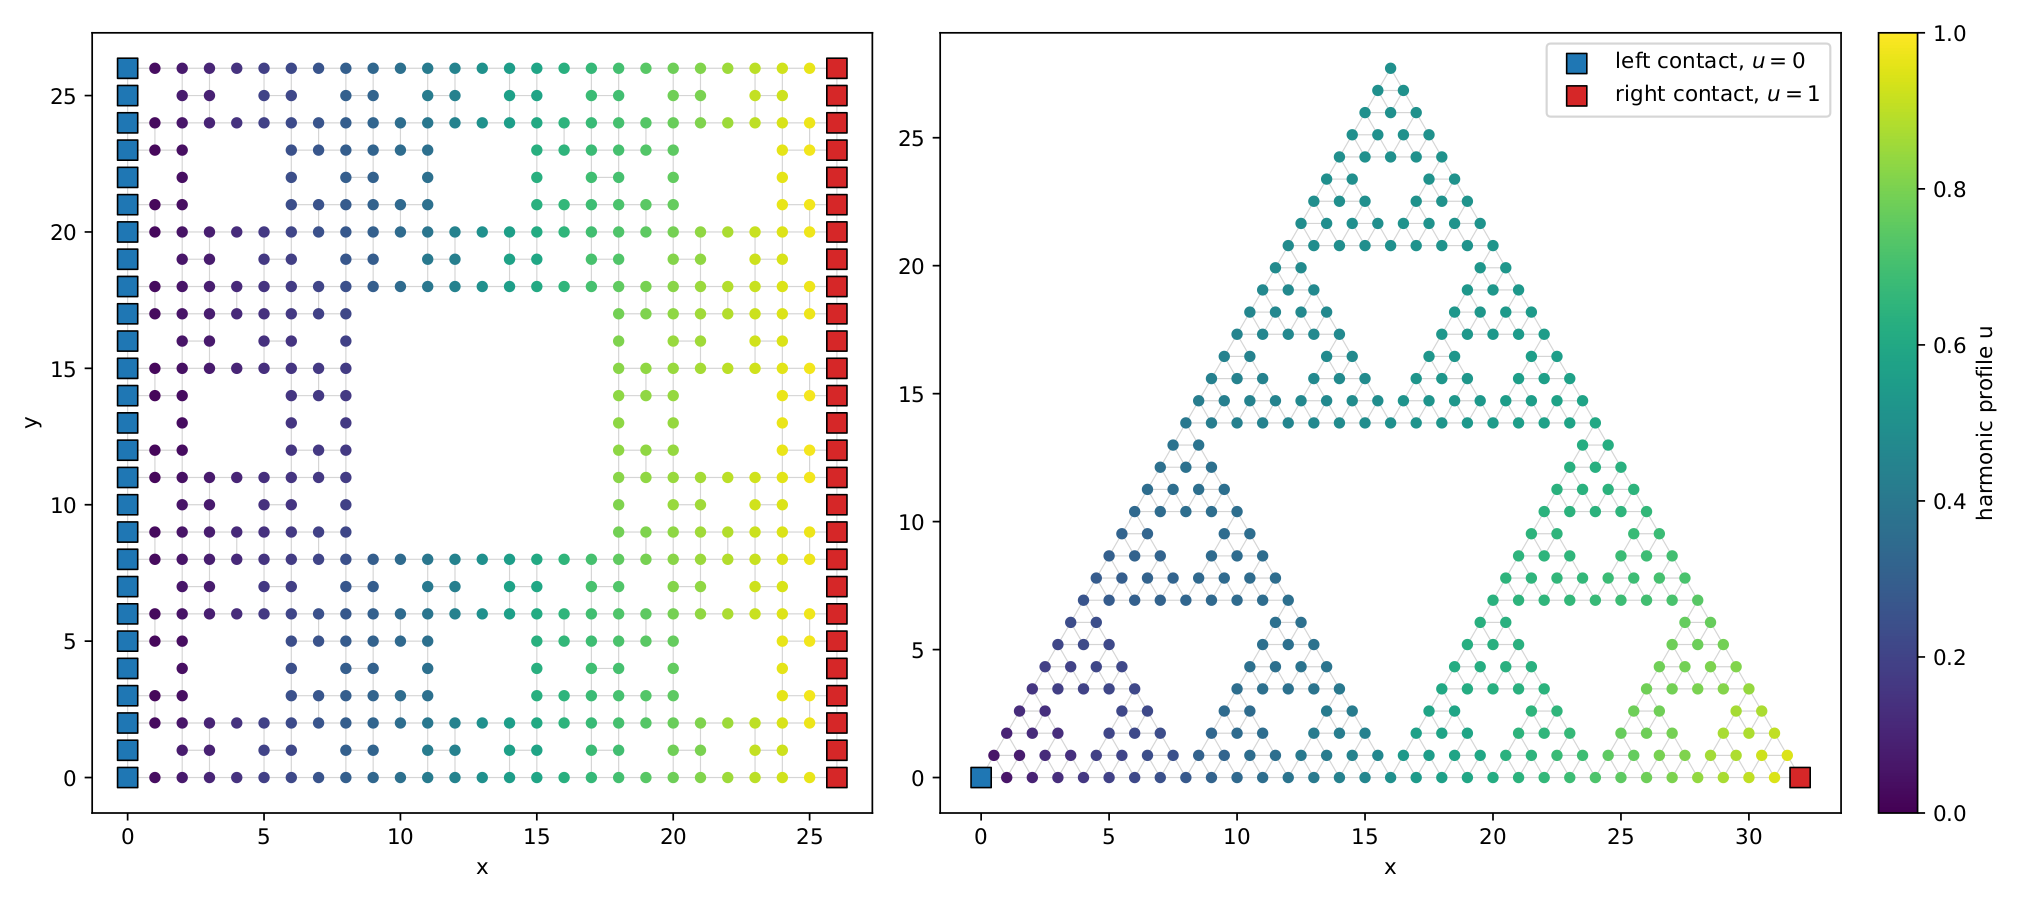
\includegraphics[width=\columnwidth]{fig_harmonic_profile.png}
\caption{Two-terminal contact geometry and discrete harmonic twist profile $u_i$ [Eq.~\eqref{eq:eq16_harmonic_u}] for the homogeneous nearest-neighbor XY model ($J_{ij} = 1$) on (left) the generation-$G=3$ Sierpi\'nski carpet ($N=512$) and (right) the generation-$G=4$ triangular Sierpi\'nski gasket ($N=366$). Blue squares mark the left lead $\mathcal{L}$ pinned at $u_i = 0$, red squares mark the right lead $\mathcal{R}$ pinned at $u_i = 1$, and interior sites are colored by their harmonic potential $u_i \in (0,1)$, which channels supercurrent around the internal fractal lacunae.}
\label{fig:harmonic_profile}
\end{figure}

Defining the $p$-th instantaneous twist derivatives of the Hamiltonian at $\phi = 0$,
\begin{equation}
H_p = \left.\frac{\partial^p H(\phi)}{\partial\phi^p}\right|_{\phi=0},
\label{eq:eq17_Hp_def}
\end{equation}
the first two derivatives represent the macroscopic twist current and the instantaneous diamagnetic stiffness,
\begin{align}
H_1 &= \sum_{\langle i,j\rangle} J_{ij} a_{ij} \sin(\theta_i - \theta_j), \label{eq:eq18_H1} \\
H_2 &= \sum_{\langle i,j\rangle} J_{ij} a_{ij}^2 \cos(\theta_i - \theta_j). \label{eq:eq19_H2}
\end{align}
(In the fermionic HMC runs P and C, $H_1 = \bm{u}\cdot\partial F/\partial\bm{\theta}$ is obtained directly from the exact Hellmann--Feynman force at zero twist without extra diagonalizations, and $H_2$ is evaluated via a central finite difference of the quasiparticle grand potential under $\Delta_i \to \Delta_i e^{\pm i h u_i}$ with $h = 0.02$.) Expanding the free energy $F(\phi) = -T\ln Z(\phi)$ in powers of the imposed twist, the second-order response defines the two-terminal phase stiffness $K_2$ ($= K_{\mathrm{open}}$):
\begin{equation}
K_2 = \left.\frac{\partial^2 F}{\partial\phi^2}\right|_{\phi=0} = \langle H_2\rangle - \frac{1}{T}\left(\langle H_1^2\rangle - \langle H_1\rangle^2\right).
\label{eq:eq20_K2}
\end{equation}
To compare lattices of different sizes, shapes, and fractal dilutions on an equal footing, we normalize $K_2$ by the two-terminal harmonic conductance $g$ (also denoted $g_0$ for unit couplings) of the network, yielding the dimensionless second-order helicity modulus (denoted interchangeably by $\Upsilon_2$, $\Upsilon$, or $\rho$):
\begin{equation}
\Upsilon_2 \equiv \rho = \frac{K_2}{g}, \qquad g = \sum_{i<j} J_{ij} a_{ij}^2.
\label{eq:eq21_Upsilon2}
\end{equation}
By virtue of Eq.~\eqref{eq:eq16_harmonic_u}, this normalization guarantees that $\Upsilon_2(T \to 0) = 1$ for unit couplings ($J_{ij} = 1$) on \emph{any} graph regardless of its fractal dimension or hole structure, and more generally that $\rho = J$ for any uniform coupling $J$.

To probe non-Gaussian phase fluctuations and the sharpness of vortex unbinding, we also evaluate the fourth-order twist response
\begin{equation}
K_4 = \left.\frac{\partial^4 F}{\partial\phi^4}\right|_{\phi=0}.
\label{eq:eq22_K4_def}
\end{equation}
Introducing the third and fourth Hamiltonian twist derivatives,
\begin{align}
H_3 &= -\sum_{\langle i,j\rangle} J_{ij} a_{ij}^3 \sin(\theta_i - \theta_j), \label{eq:eq23_H3} \\
H_4 &= -\sum_{\langle i,j\rangle} J_{ij} a_{ij}^4 \cos(\theta_i - \theta_j), \label{eq:eq24_H4}
\end{align}
and writing $\delta H_p = H_p - \langle H_p\rangle$, the complete cumulant estimator for $K_4$ is
\begin{equation}
K_4 = \langle H_4\rangle - \frac{1}{T}\left[ 4\langle \delta H_1 \delta H_3\rangle + 3\langle (\delta H_2)^2\rangle \right] + \frac{6}{T^2}\left\langle \delta H_2 (\delta H_1)^2\right\rangle - \frac{1}{T^3}\left[ \langle (\delta H_1)^4\rangle - 3\langle (\delta H_1)^2\rangle^2 \right],
\label{eq:eq25_K4_full}
\end{equation}
which retains the measured sample means of the odd derivatives without assuming their exact vanishing in a finite trajectory. In the phase-inversion-symmetric equilibrium ensemble, the twist free energy expands as
\begin{equation}
F(\phi) - F(0) = \frac{K_2}{2}\phi^2 + \frac{K_4}{4!}\phi^4 + \mathcal{O}(\phi^6),
\label{eq:eq26_F_expansion}
\end{equation}
and normalizing $K_4$ by the same geometric conductance $g$ defines the fourth-order helicity modulus
\begin{equation}
\Upsilon_4 = \frac{K_4}{g}.
\label{eq:eq27_Upsilon4}
\end{equation}
In a two-dimensional BKT transition, the discontinuous drop of $\Upsilon_2(T)$ across $T_{\mathrm{BKT}}$ is accompanied by a sharp negative dip (minimum) in $\Upsilon_4(T)$ that deepens with system size~\cite{Minnhagen2003}.

Finally, to locate the finite-size phase-coherence crossover temperature $T_\times$ (or $T_A, T_B, T_P, T_C$ for the four microscopic rungs) from the continuous curve $\rho(T)$, we apply three complementary criteria:
\begin{enumerate}
\item \emph{Standard BKT crossing (``coded'' criterion):} the intersection $\rho(T_\times) = 2T_\times/\pi$ of the conductance-normalized two-terminal stiffness with the universal Nelson--Kosterlitz line~\cite{NK77}. We adopt this as our primary baseline across all lattices.
\item \emph{Sheet-rescaled criterion:} on a translationally invariant two-dimensional lattice, the continuum sheet stiffness carries a coordination geometry factor $\sigma J$ ($\sigma = 1, \sqrt{3}, 1/\sqrt{3}$ for the square, triangular, and honeycomb lattices), shifting the universal jump line to $\rho(T) = 2T/(\pi\sigma)$. Although a fractal lacks a continuum sheet stiffness, one can define an effective geometric sheet factor $s = \sigma_{\mathrm{parent}}\, g_0 / g_{0,\mathrm{parent}}$ to test sensitivity to continuum rescaling.
\item \emph{Half-stiffness criterion $T_{50}$:} the temperature at which thermal fluctuations reduce the stiffness to half of the same model's no-fluctuation reference value ($\rho(T_{50})/\rho_{\mathrm{ref}}(T_{50}) = 1/2$, with $\rho_{\mathrm{ref}} = \rho_{\mathrm{harm}}$ for Rung~B and $\rho_{\mathrm{ref}} = \rho_A$ for Rungs~P and~C). Because the normalization $g_0$ cancels identically in the ratio $\rho/\rho_{\mathrm{ref}}$, $T_{50}$ is completely independent of any geometric conductance convention.
\end{enumerate}

%======================================================================
\section{Uniform Nearest-Neighbor XY Model on Fractal Structures}
\label{sec:uniform_xy}
%======================================================================

Before turning to the inhomogeneous, temperature-dependent couplings generated by the attractive Hubbard model, it is essential to understand how fractal geometry alone reshapes thermal phase fluctuations and vortex unbinding when every nearest-neighbor bond carries a uniform ferromagnetic coupling $J_{ij} = J = 1$. To this end, we perform extensive hybrid Wolff--Metropolis simulations across five generations of the Sierpi\'nski carpet ($G = 1, \dots, 5$, spanning $N = 8$ to $N = 32\,768$ sites) and seven generations of the triangular and honeycomb Sierpi\'nski gaskets ($G = 1, \dots, 7$, spanning up to $N = 9843$ and $N = 16\,404$ sites, respectively).

\begin{figure}[t]
\centering
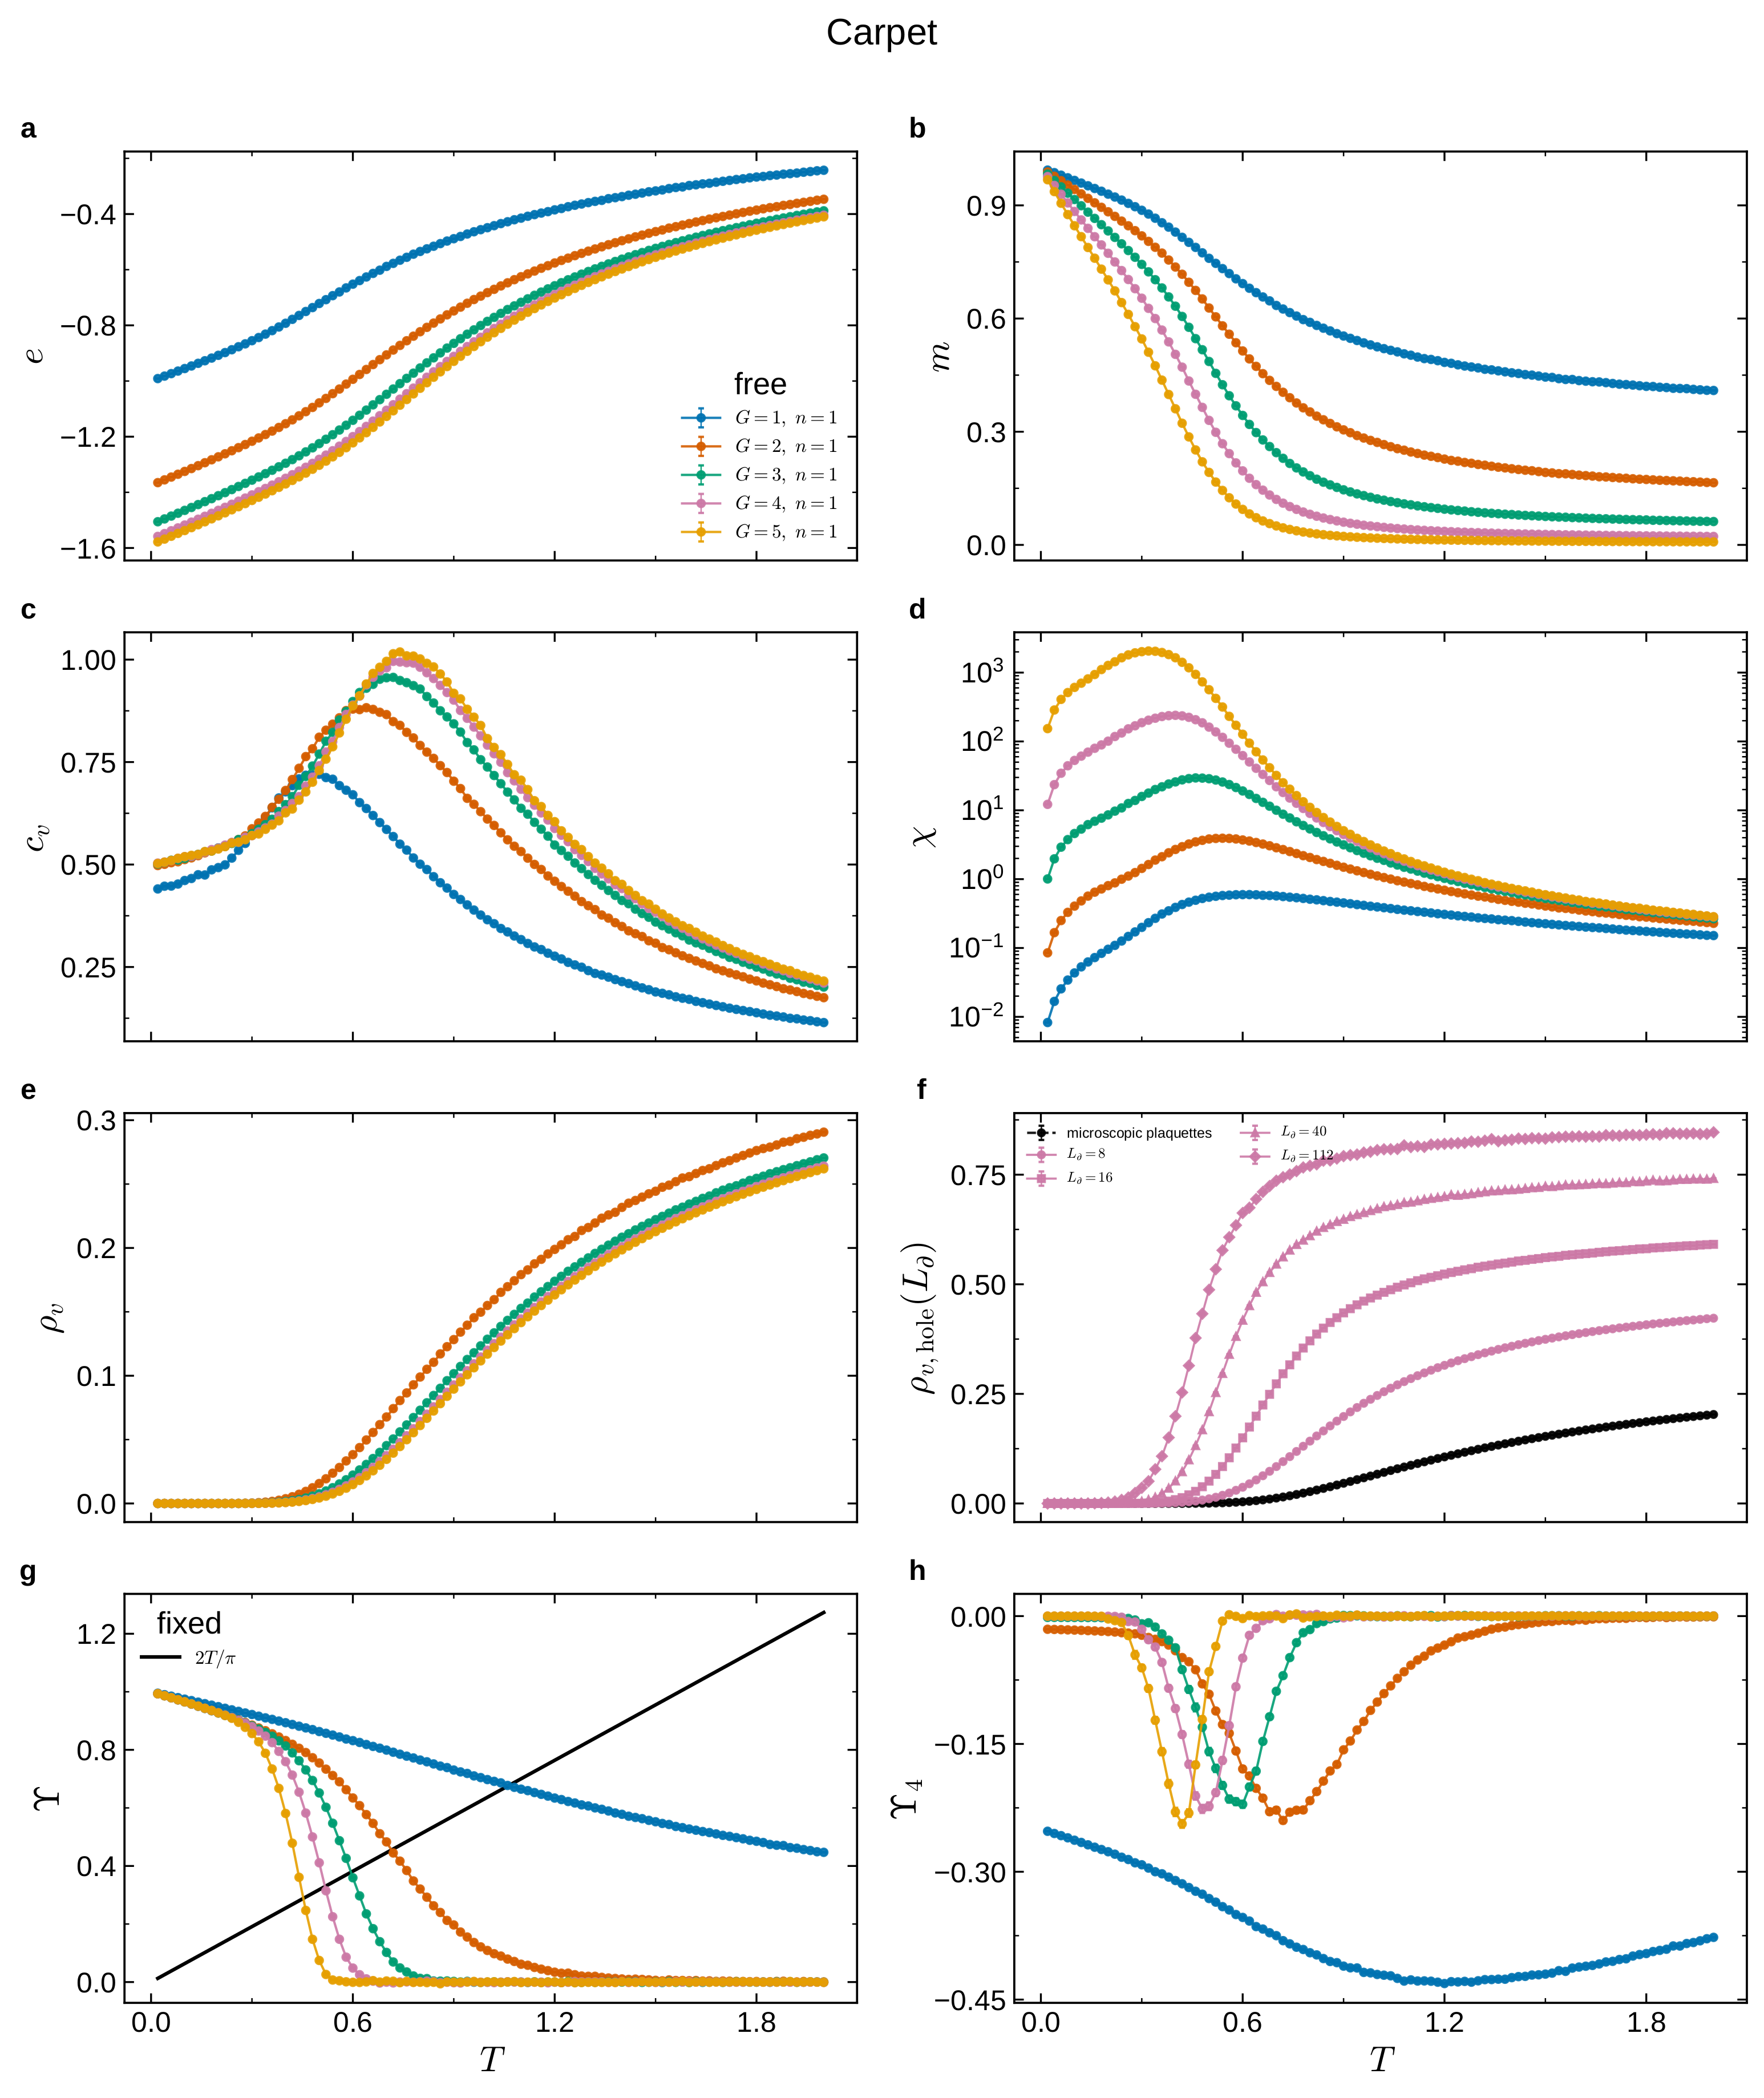
\includegraphics[width=\columnwidth]{fig_uniform_xy_carpet_panel.png}
\caption{Thermodynamics and two-terminal phase response of the uniform nearest-neighbor XY model ($J = 1$) on the Sierpi\'nski carpet across generations $G = 1, \dots, 5$ ($n = 1$). Panels~(a)--(f) show free-boundary observables as functions of temperature $T$: (a)~mean energy per site $e$, (b)~magnetization magnitude $m$, (c)~specific heat $c_V$, (d)~magnetic susceptibility $\chi$ on a logarithmic scale, (e)~total vortex density $\rho_v$ across all faces, and (f)~scale-resolved vortex occupation $\rho_{v,\mathrm{hole}}(L_\partial)$ on internal lacunae of perimeter $L_\partial = 8, 16, 40, 112$ compared against elementary microscopic plaquettes ($L_\partial = 4$, black curve) for $G=4$. Panels~(g) and~(h) show fixed-contact two-terminal transport observables: (g)~the normalized second-order helicity modulus $\Upsilon \equiv \Upsilon_2$ together with the universal BKT line $2T/\pi$, and (h)~the fourth-order helicity modulus $\Upsilon_4$.}
\label{fig:uniform_carpet_panel}
\end{figure}

\begin{figure}[t]
\centering
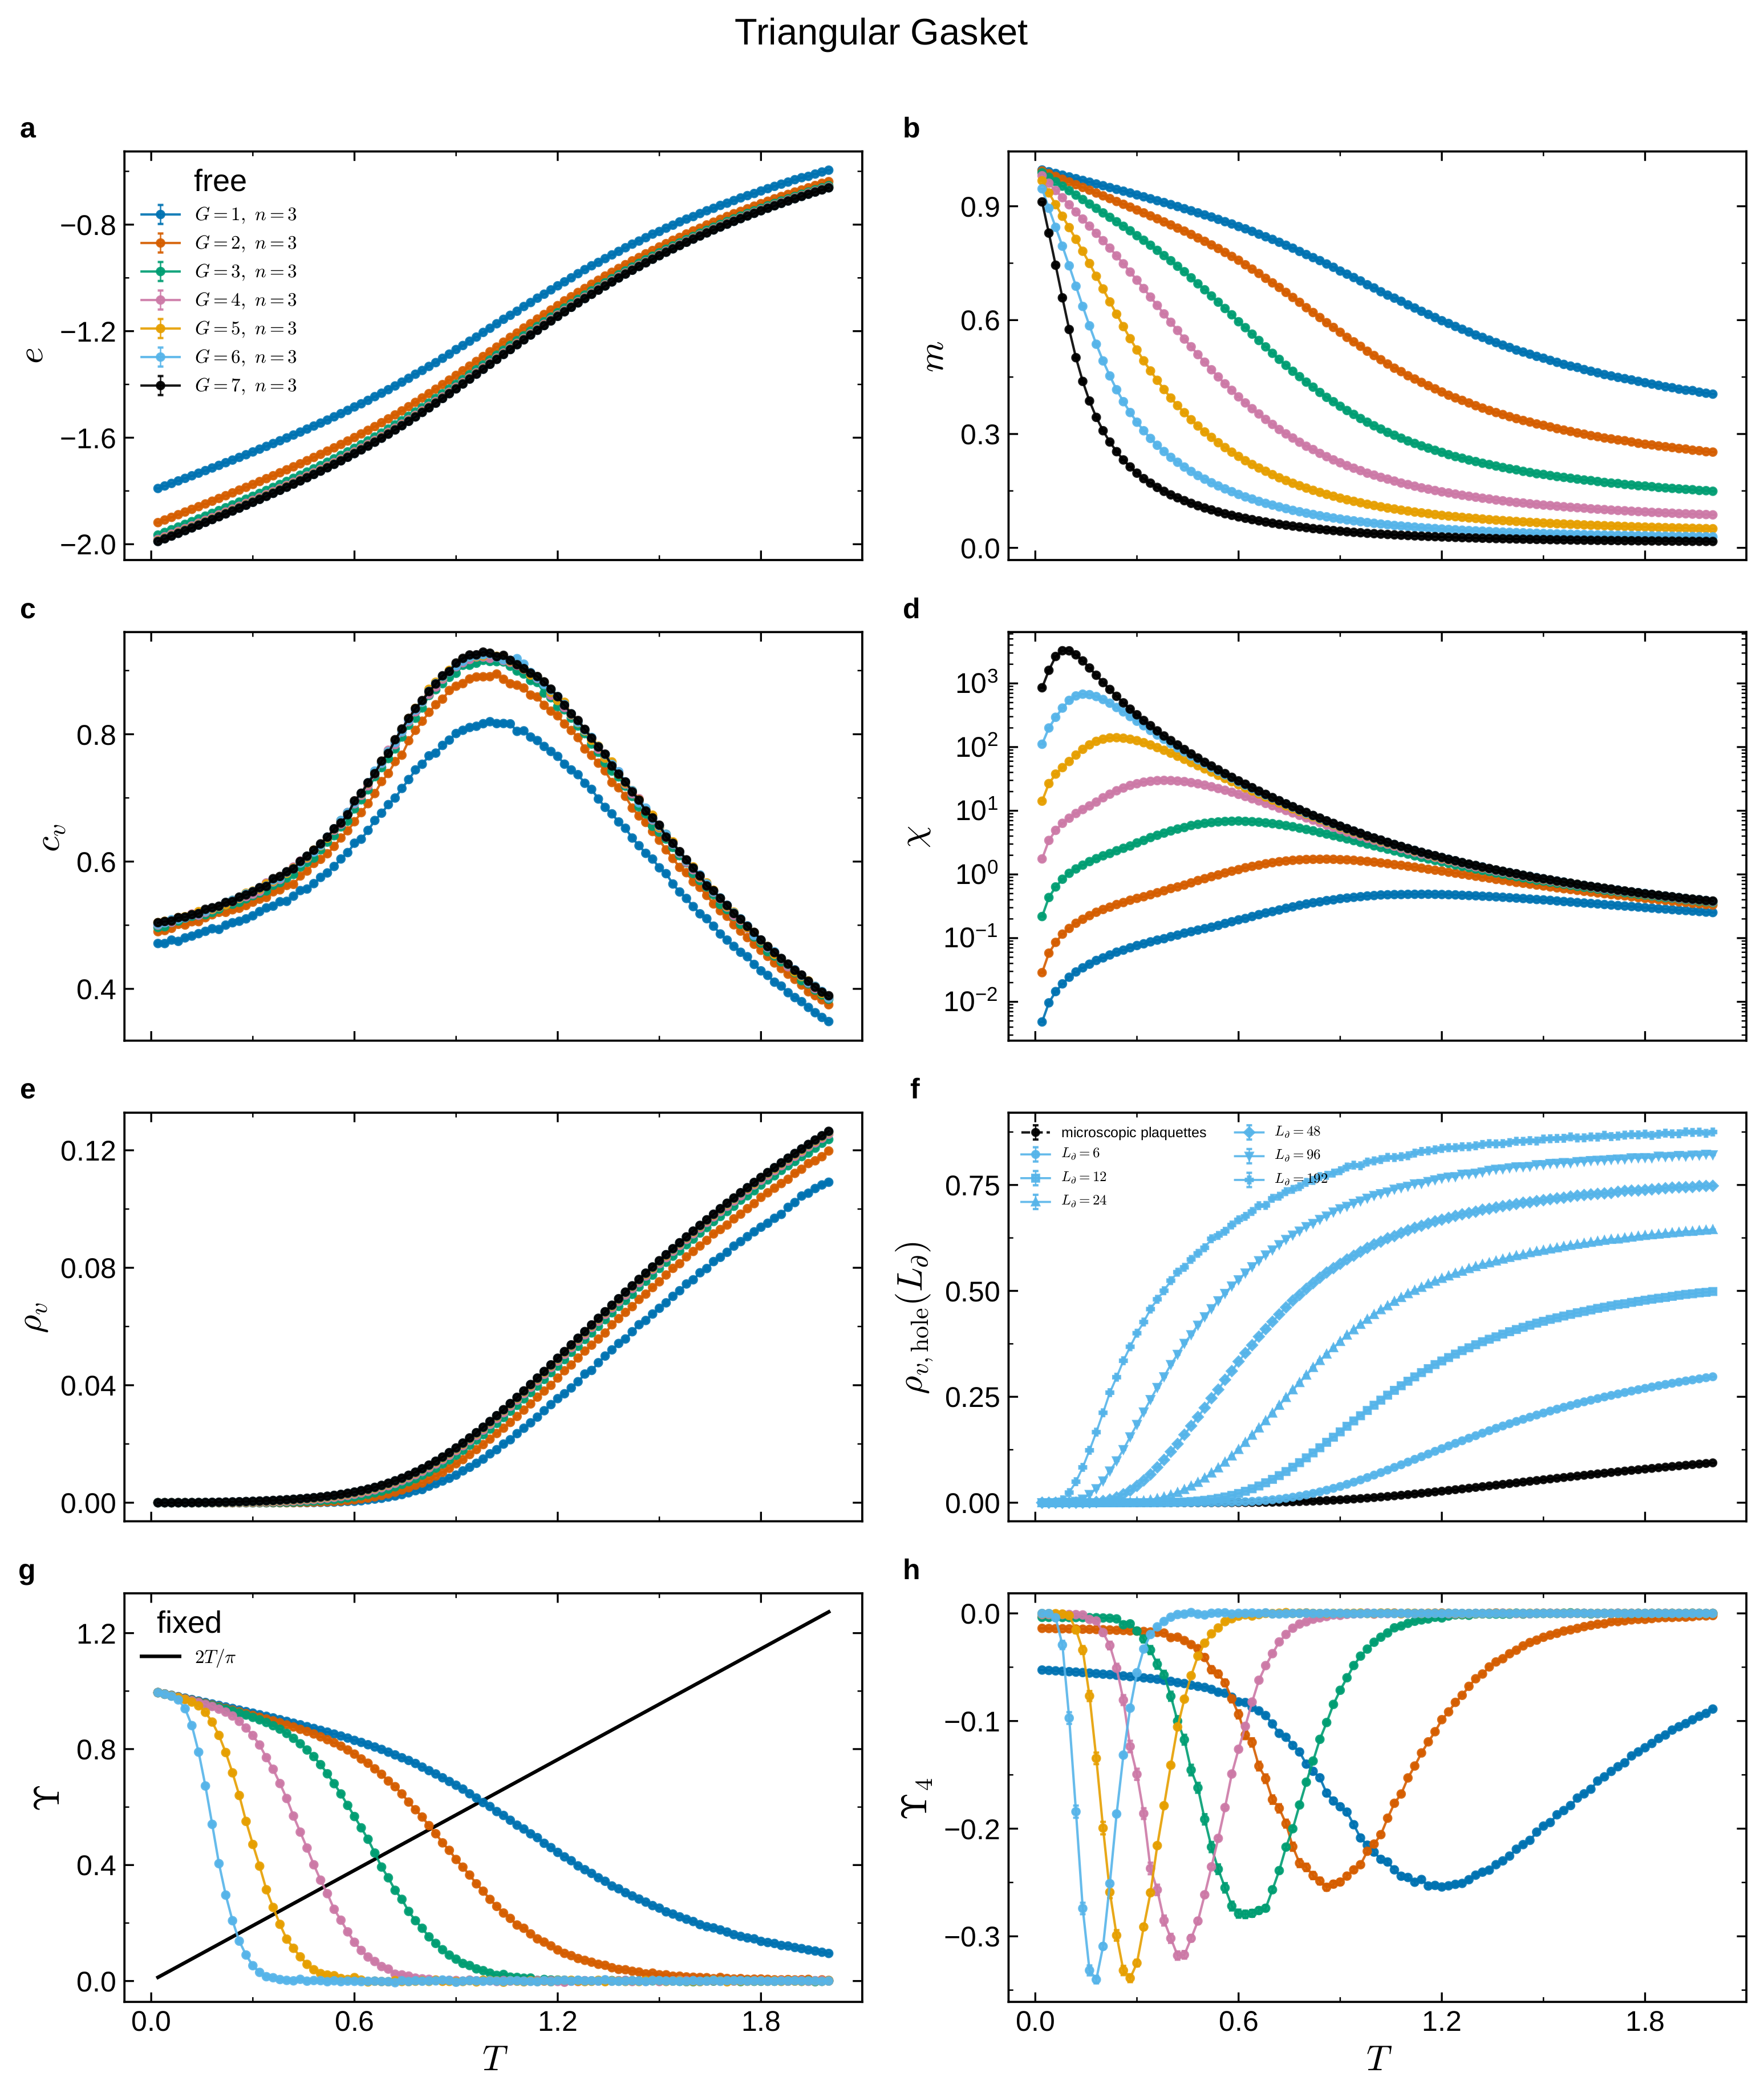
\includegraphics[width=\columnwidth]{fig_uniform_xy_triangular_panel.png}
\caption{Thermodynamics and two-terminal phase response of the uniform nearest-neighbor XY model ($J = 1$) on the triangular Sierpi\'nski gasket across generations $G = 1, \dots, 7$ ($n = 3$). Panels~(a)--(h) follow the same layout as Fig.~\ref{fig:uniform_carpet_panel}, with panel~(f) resolving the vortex density $\rho_{v,\mathrm{hole}}(L_\partial)$ across triangular lacunae of perimeter $L_\partial = 6, 12, 24, 48, 96, 192$ versus elementary microscopic triangles ($L_\partial = 3$, black curve).}
\label{fig:uniform_triangular_panel}
\end{figure}

\begin{figure}[t]
\centering
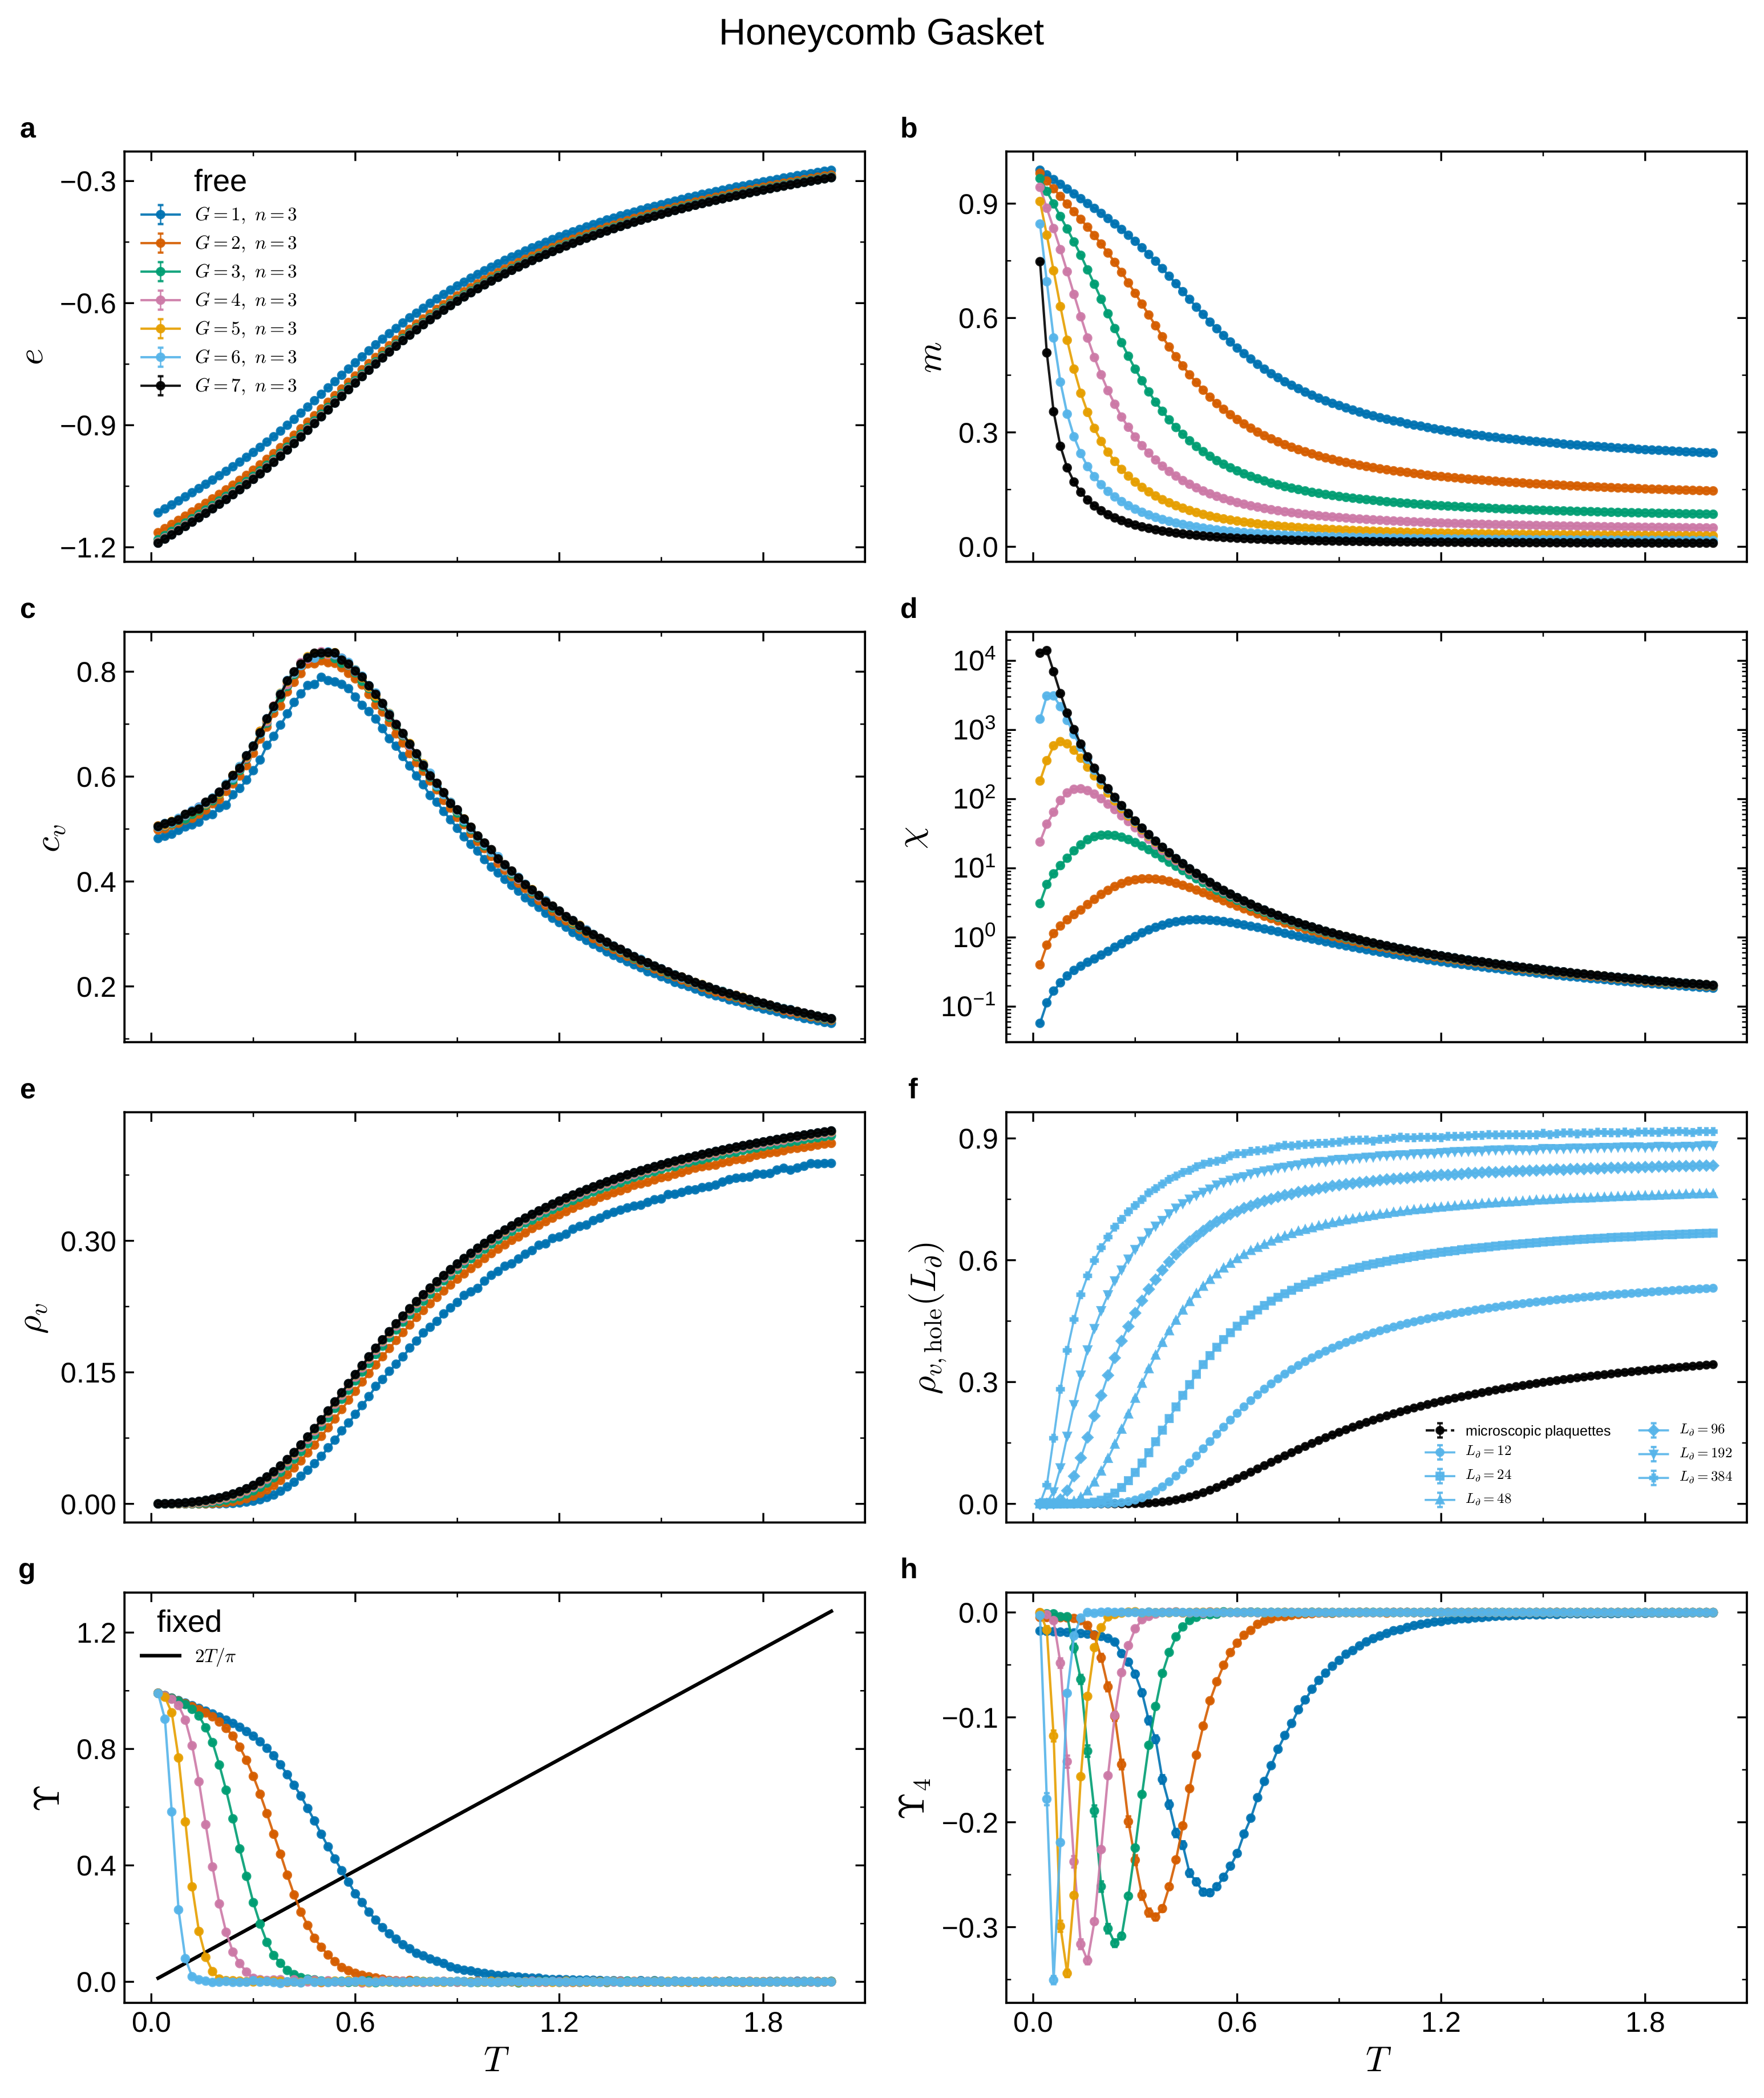
\includegraphics[width=\columnwidth]{fig_uniform_xy_honeycomb_panel.png}
\caption{Thermodynamics and two-terminal phase response of the uniform nearest-neighbor XY model ($J = 1$) on the honeycomb Sierpi\'nski gasket across generations $G = 1, \dots, 7$ ($n = 3$). Panels~(a)--(h) follow the same layout as Figs.~\ref{fig:uniform_carpet_panel} and~\ref{fig:uniform_triangular_panel}, with panel~(f) resolving the vortex density across hexagonal lacunae of perimeter $L_\partial = 12, 24, 48, 96, 192, 384$ versus elementary hexagons ($L_\partial = 6$, black curve).}
\label{fig:uniform_honeycomb_panel}
\end{figure}

Figures~\ref{fig:uniform_carpet_panel}, \ref{fig:uniform_triangular_panel}, and~\ref{fig:uniform_honeycomb_panel} present the complete thermodynamic and transport portraits of the Sierpi\'nski carpet, the triangular gasket, and the honeycomb gasket, respectively. Comparing the eight panels across the three fractal families reveals a striking separation between short-wavelength energetics and macroscopic phase coherence. In all three geometries, the mean energy per site $e(T)$ [panel~(a)] and the specific heat $c_V(T)$ [panel~(c)] rapidly converge with generation $G$ to smooth, size-independent limiting curves. At low temperatures, $c_V(T)$ approaches the classical equipartition value $1/2$ per spin expected for harmonic spin waves, before rising to a broad round maximum at a temperature $T_{\max c_V}$ ($\simeq 0.74$ on the carpet, $\simeq 1.00$ on the triangular gasket, and $\simeq 0.52$ on the honeycomb gasket) that reflects the local build-up of short-range nearest-neighbor phase correlations on elementary sub-blocks. Crucially, the height of this specific-heat peak shows no divergence with system size on any of the three fractals, confirming that the onset of local spin-wave correlations is a non-critical crossover.

In sharp contrast, the observables sensitive to long-wavelength phase order---the finite-size magnetization $m(T)$ [panel~(b)], the susceptibility $\chi(T)$ [panel~(d)], the two-terminal helicity modulus $\Upsilon(T)$ [panel~(g)], and the fourth-order modulus $\Upsilon_4(T)$ [panel~(h)]---shift systematically toward lower temperatures as the fractal generation $G$ increases. At the same time, the susceptibility maximum $\max_T \chi$ grows by roughly an order of magnitude per generation on the logarithmic scale of panel~(d), reflecting the expanding domain over which phases remain correlated at low temperatures.

The microscopic mechanism driving the loss of phase coherence is exposed by the topological vortex densities in panels~(e) and~(f) of Figs.~\ref{fig:uniform_carpet_panel}--\ref{fig:uniform_honeycomb_panel}, together with the real-space spin and vorticity snapshots shown in Fig.~\ref{fig:snapshots_all}. While the total vortex density $\rho_v(T)$ averaged over all faces [panel~(e)] appears to turn on only at relatively high temperatures near $T_{\max c_V}$, this average is numerically dominated by the vast number of elementary microscopic plaquettes ($L_\partial = 3, 4, 6$). When the vortex population is decomposed by hole perimeter $L_\partial$ in panel~(f), a dramatic hierarchical ordering emerges: \emph{vortices populate the largest fractal lacunae at temperatures several times lower than the onset of microscopic plaquette vortices}, and each successively smaller scale of lacuna activates at a progressively higher temperature.

\begin{figure*}[t]
\centering
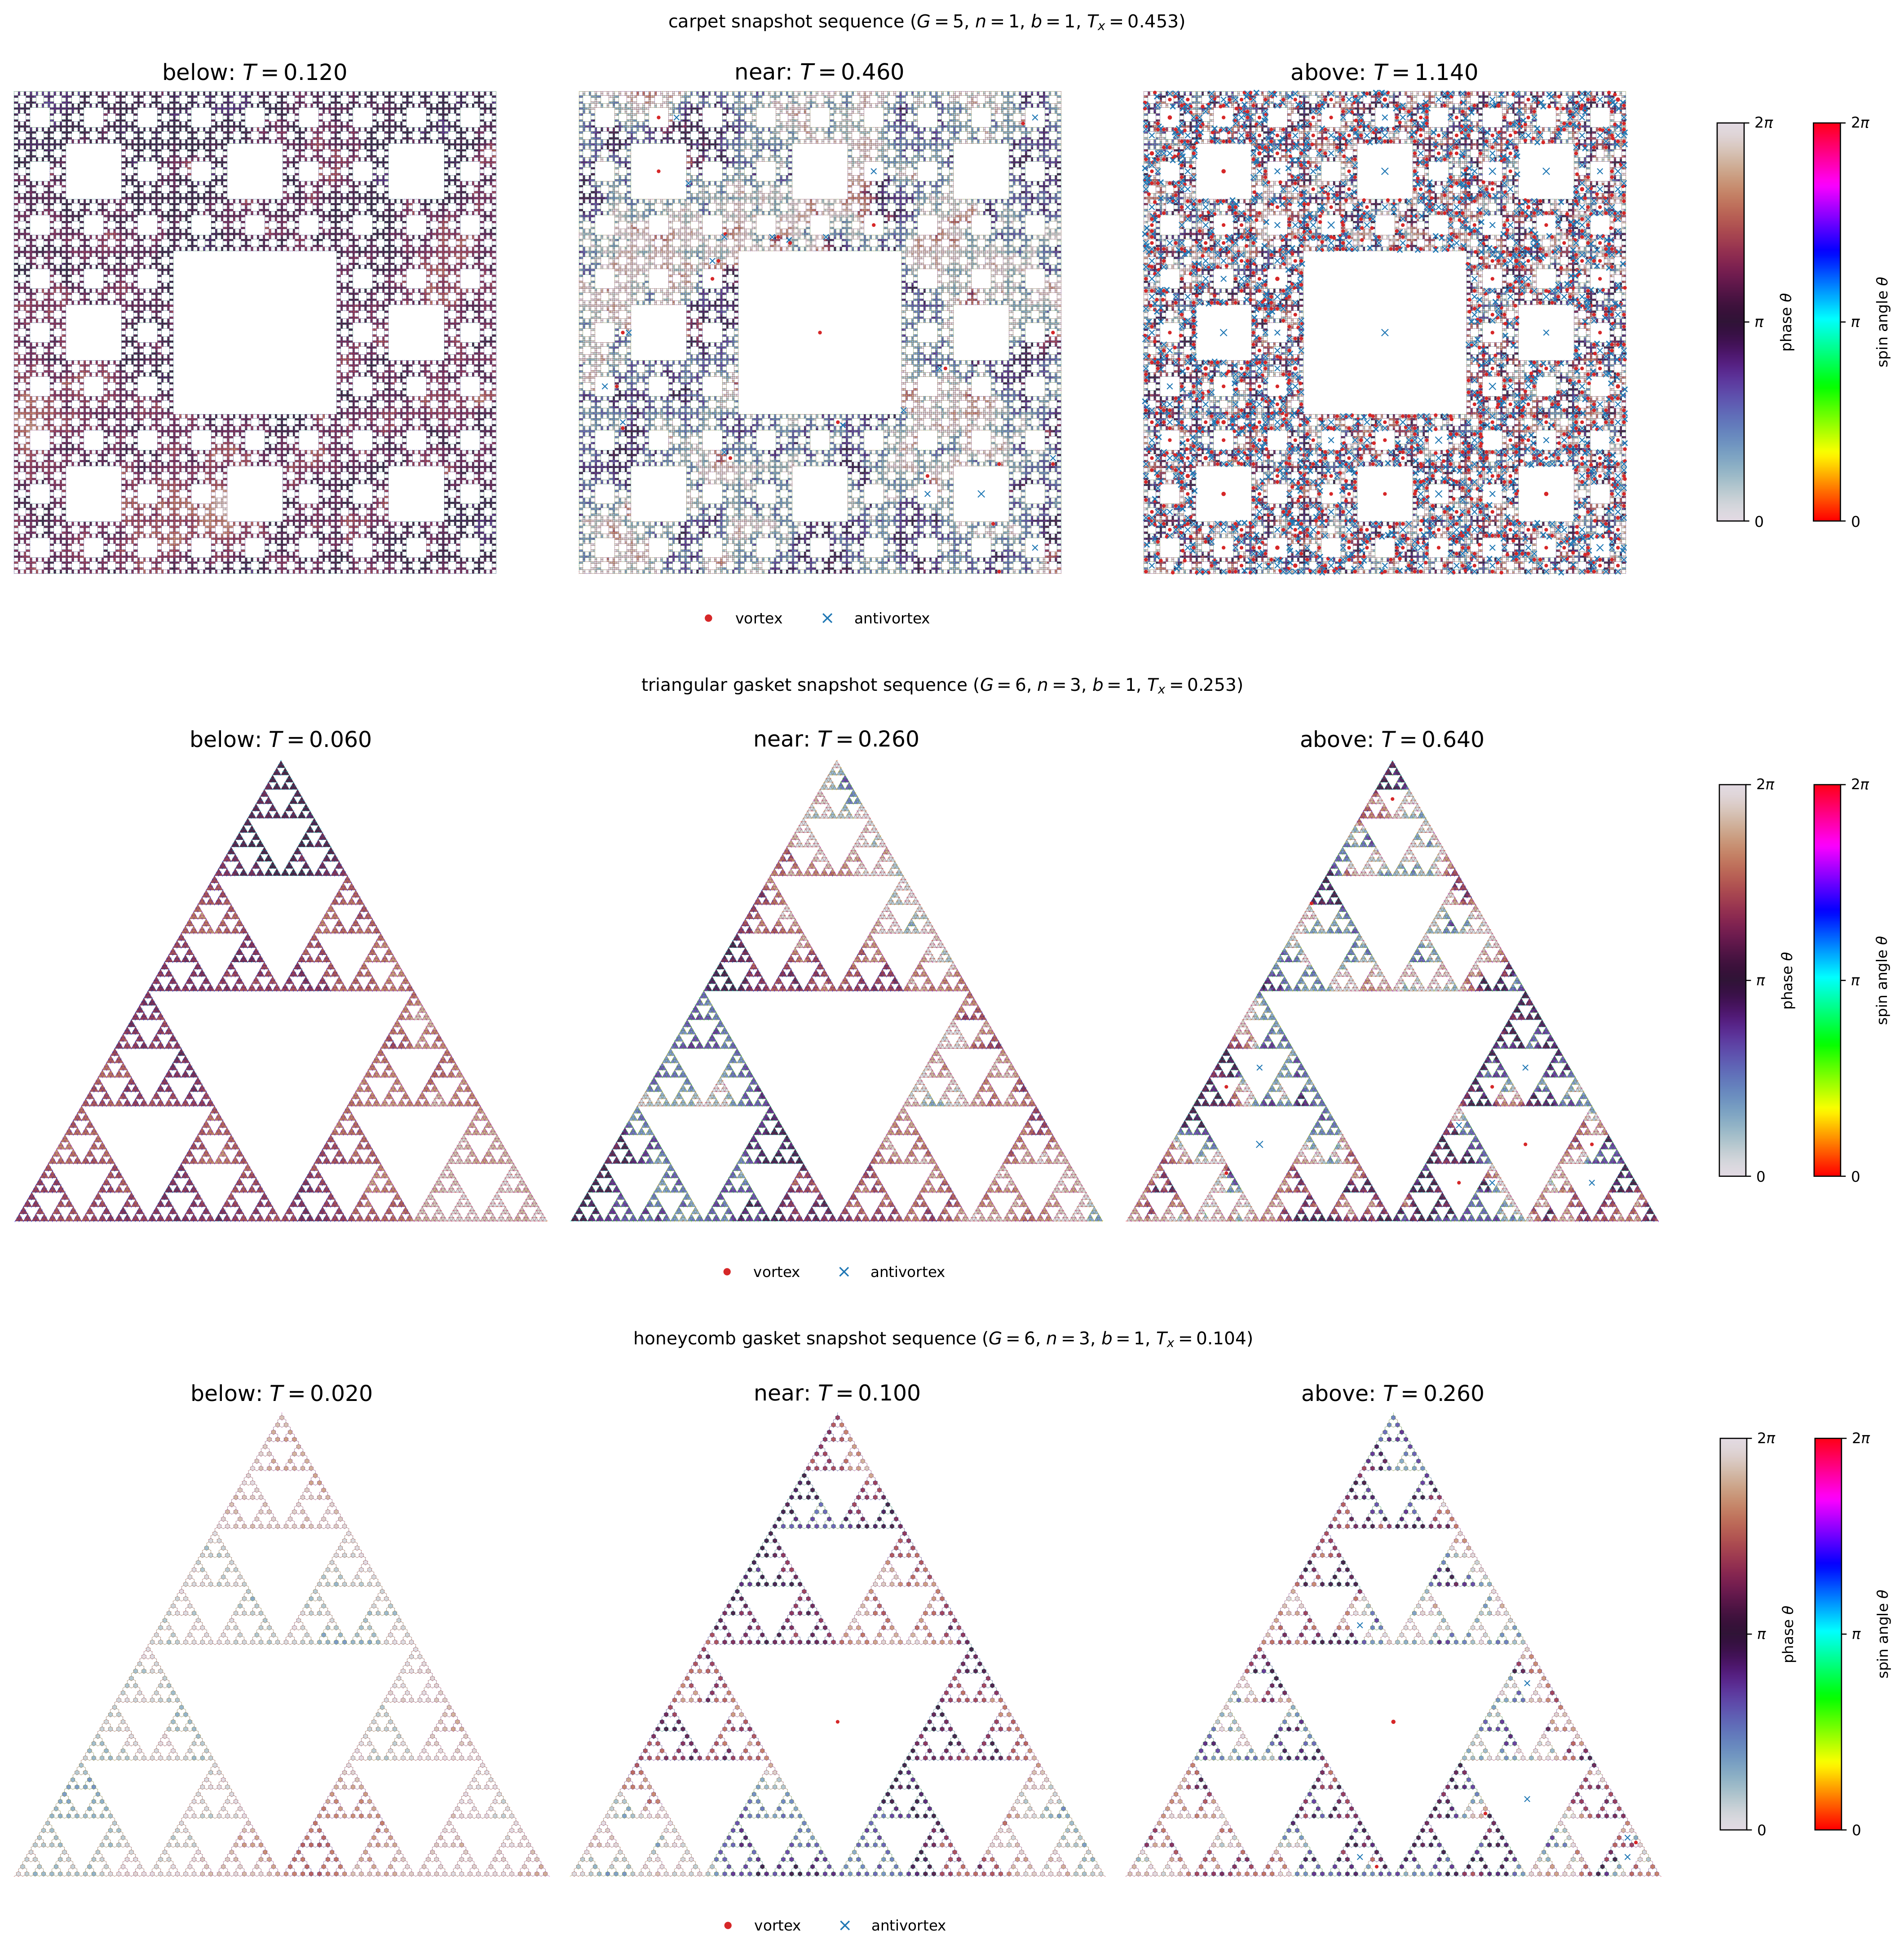
\includegraphics[width=0.95\textwidth]{fig_snapshots_all.png}
\caption{Representative real-space Monte Carlo configurations of the uniform nearest-neighbor XY model ($J=1$) at three characteristic temperatures---well below ($T \simeq 0.25\, T_\times$, left column), immediately near ($T \simeq T_\times$, middle column), and well above ($T \simeq 2.5\, T_\times$, right column) the finite-size helicity crossover temperature $T_\times$---for (top row) the $G=5$ Sierpi\'nski carpet ($T_\times = 0.453$), (middle row) the $G=6$ triangular Sierpi\'nski gasket ($T_\times = 0.253$), and (bottom row) the $G=6$ honeycomb Sierpi\'nski gasket ($T_\times = 0.104$). Site colors and quivers encode the local phase angle $\theta_i \in [0, 2\pi)$, while red circles and blue crosses mark the topological charges $q_f = +1$ (vortices) and $q_f = -1$ (antivortices) on elementary plaquettes and internal fractal lacunae. Near $T_\times$ (middle column), elementary plaquettes remain essentially vortex-free while topological charges selectively occupy the large central and secondary lacunae.}
\label{fig:snapshots_all}
\end{figure*}

The physical origin of this scale hierarchy is straightforward. A vortex of unit winding $q_f = \pm 1$ circulating around a lacuna of perimeter $L_\partial$ distributes its $2\pi$ phase wind across roughly $L_\partial$ boundary bonds, so the local phase gradient scales as $\nabla\theta \sim 2\pi / L_\partial$ and the coreless harmonic energy cost decreases rapidly with increasing hole perimeter. As confirmed visually by the middle column of Fig.~\ref{fig:snapshots_all}, at the crossover temperature $T \simeq T_\times$ where the two-terminal superfluid stiffness collapses, the bulk of the fractal fabric is still locally smooth and free of microscopic plaquette vortices; instead, phase coherence across the flake is destroyed by vortices and antivortices sitting inside the primary and secondary lacunae, which thread $2\pi$ phase slips between the left and right contacts. Below $T_\times$ (left column of Fig.~\ref{fig:snapshots_all}), even the largest lacunae are empty and the phase maintains quasi-uniform alignment across the entire sample; well above $T_\times$ (right column), smaller lacunae and elementary plaquettes also fill with unbound topological charges.

\begin{figure}[t]
\centering
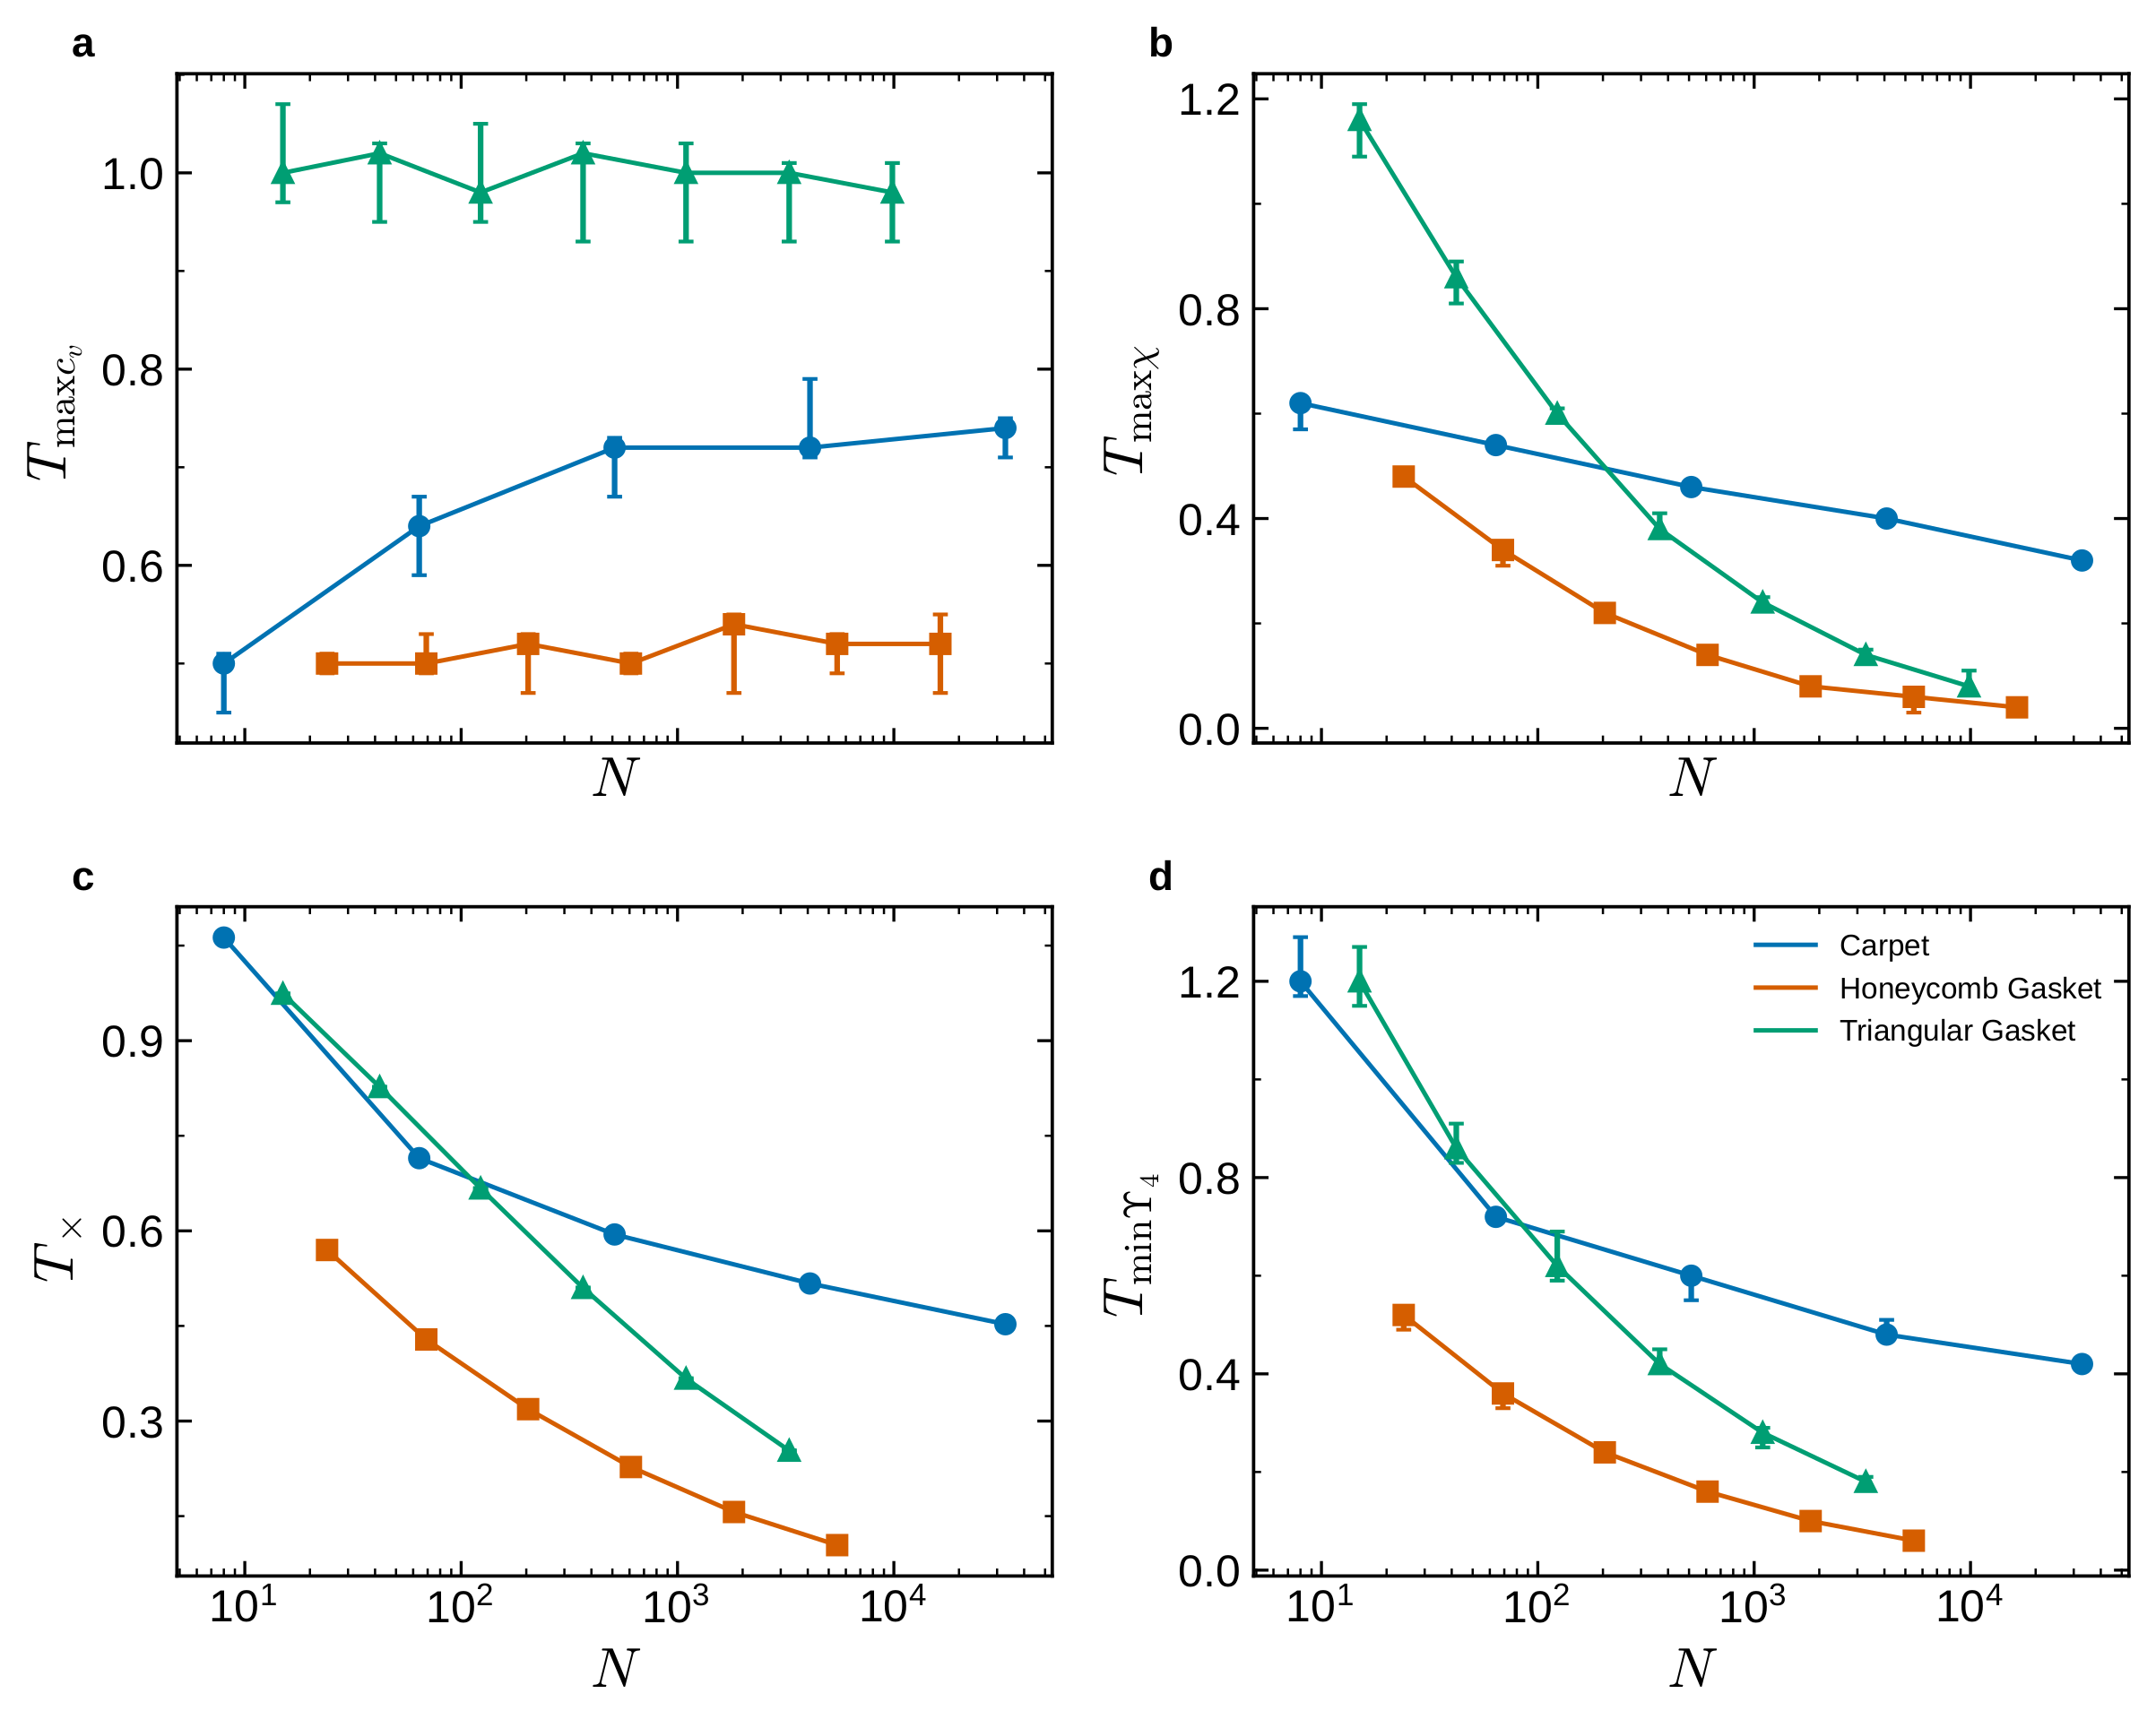
\includegraphics[width=\columnwidth]{fig_uniform_xy_extrema_scaling.png}
\caption{System-size scaling of the four characteristic temperatures of the uniform nearest-neighbor XY model ($J=1$) plotted against total site count $N$ on a logarithmic scale for the Sierpi\'nski carpet (blue circles, $G=1\dots 5$), the honeycomb Sierpi\'nski gasket (orange squares, $G=1\dots 7$), and the triangular Sierpi\'nski gasket (green triangles, $G=1\dots 7$): (a)~specific-heat peak temperature $T_{\max c_V}$, (b)~susceptibility peak temperature $T_{\max \chi}$, (c)~two-terminal BKT helicity crossing temperature $T_\times$, and (d)~location of the fourth-order helicity minimum $T_{\min \Upsilon_4}$.}
\label{fig:extrema_scaling}
\end{figure}

\begin{figure*}[t]
\centering
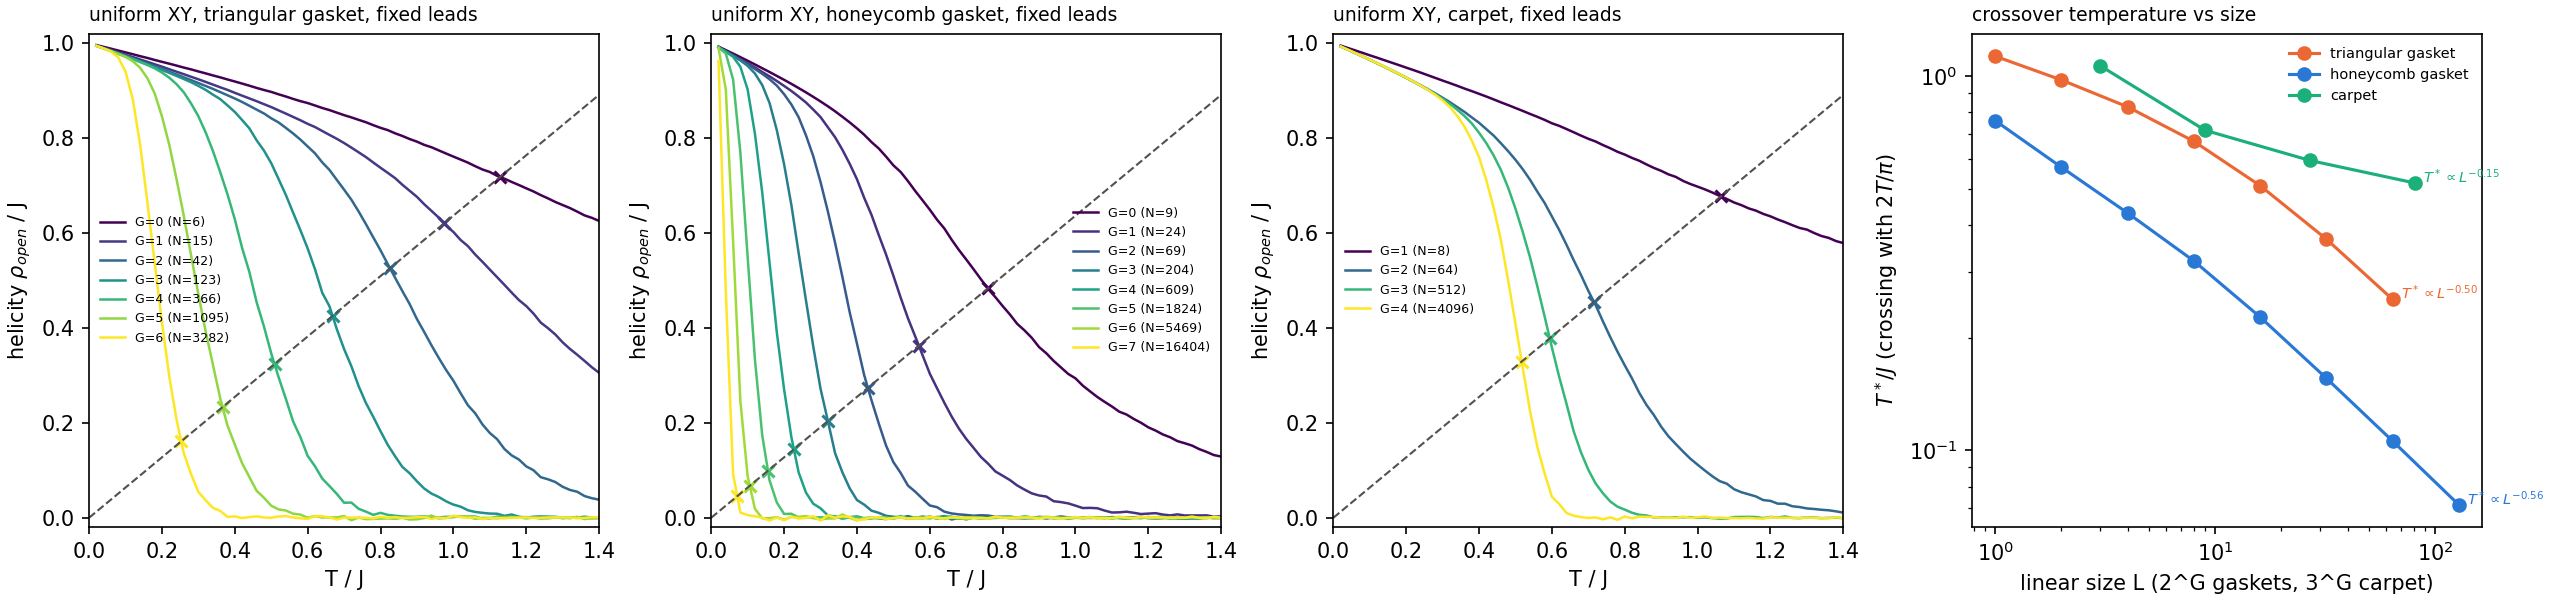
\includegraphics[width=0.96\textwidth]{uniform_xy_size_scaling.png}
\caption{Generation dependence of the fixed-lead two-terminal helicity modulus $\rho_{\mathrm{open}}/J \equiv \Upsilon_2$ for the uniform nearest-neighbor XY model on (first panel) the triangular gasket ($G=0\dots 6$), (second panel) the honeycomb gasket ($G=0\dots 7$), and (third panel) the Sierpi\'nski carpet ($G=1\dots 4$), together with the universal BKT line $2T/\pi$ (dashed black line; crosses mark the intersections $T^* \equiv T_\times$). The fourth panel plots the dimensionless crossover temperature $T^*/J$ on a double-logarithmic scale against the linear sample size $L$ ($L = 2^G$ for the gaskets, $L = 3^G$ for the carpet), revealing power-law decays $T^* \propto L^{-x}$ with $x \approx 0.50$ (triangular gasket), $x \approx 0.56$ (honeycomb gasket), and a much weaker drift $x \approx 0.15$ on the infinitely ramified carpet.}
\label{fig:uniform_size_scaling}
\end{figure*}

To quantify how the coherence scale evolves with fractal generation, Fig.~\ref{fig:extrema_scaling} compares the system-size dependence of the four characteristic temperatures---$T_{\max c_V}$, $T_{\max \chi}$, the helicity crossing $T_\times$, and the fourth-order helicity minimum $T_{\min \Upsilon_4}$---as functions of total site count $N$, while Fig.~\ref{fig:uniform_size_scaling} plots the helicity crossing temperature $T^*(G) \equiv T_\times(G)$ on a double-logarithmic scale against the linear sample size $L$ ($L = 2^G$ for the gaskets and $L = 3^G$ for the carpet). Across all three fractals, the three phase-coherence diagnostics $T_{\max \chi}$, $T_\times$, and $T_{\min \Upsilon_4}$ track one another closely and decouple completely from the generation-independent local scale $T_{\max c_V}$. Moreover, the fourth-order modulus $\Upsilon_4(T)$ [panel~(h) of Figs.~\ref{fig:uniform_carpet_panel}--\ref{fig:uniform_honeycomb_panel}] develops a pronounced negative trough whose minimum position $T_{\min \Upsilon_4}$ coincides with the steepest drop of $\Upsilon_2(T)$ and approaches a finite asymptotic depth ($\min_T \Upsilon_4 \simeq -0.24$ on the carpet and $\simeq -0.34$ to $-0.35$ on the gaskets), signaling that the loss of two-terminal stiffness is driven by collective non-Gaussian vortex fluctuations rather than smooth Gaussian spin-wave softening.

Most importantly, Fig.~\ref{fig:uniform_size_scaling} highlights the fundamental contrast between finite and infinite ramification:
\begin{enumerate}
\item On the finitely ramified \emph{triangular and honeycomb Sierpi\'nski gaskets}, a vortex entering or escaping the largest central lacuna of generation $G$ must traverse a corner bottleneck whose width does not grow with $G$. As a result, the energy barrier for phase slips across the flake saturates with generation~\cite{Vallat1991,MB10}, and the finite-size coherence crossover temperature decays as a clean power law of the linear dimension,
\begin{equation}
T^*(G) \propto L^{-x},
\label{eq:Tstar_powerlaw}
\end{equation}
with exponents $x \approx 0.50$ on the triangular gasket and $x \approx 0.56$ on the honeycomb gasket. Because the linear size doubles with each generation ($L = 2^G$), every additional generation reduces the gasket crossover temperature by a factor of $2^{-x} \simeq 0.71$ (triangular) or $0.68$ (honeycomb), driving $T^*(G)/J$ down to $0.25$ at $G=6$ on the triangular gasket and down to $0.07$ at $G=7$ on the honeycomb gasket. Note also that at any fixed generation $G$, the honeycomb gasket has a crossover temperature roughly half that of the triangular gasket, because its elementary hexagonal rings have lower coordination ($z = 3$ or $2$ versus $z = 4$ or $3$) and double the bond perimeter around every lacuna, halving the effective loop stiffness.
\item On the infinitely ramified \emph{Sierpi\'nski carpet}, by contrast, the wall separating the central lacuna from the outer boundary thickens as $3^G$ while its connectivity scales as $2^G$. Consequently, the helicity curves in Fig.~\ref{fig:uniform_carpet_panel}(g) and the third panel of Fig.~\ref{fig:uniform_size_scaling} compress much more slowly with generation: an empirical power-law fit over $G = 2$--$5$ yields an effective drift exponent of only $x \approx 0.15$ ($T^*/J = 0.715, 0.594, 0.517, 0.453$ for $G = 2, 3, 4, 5$). Over the accessible range of sizes, this slow downward drift is comparable to the logarithmic finite-size shift $T^*(L) - T_{\mathrm{BKT}} \propto (\ln L)^{-2}$ of a regular two-dimensional BKT transition, leaving the carpet far more resilient to thermal phase fluctuations at any realistic mesoscopic size than the finitely ramified gaskets.
\end{enumerate}

This uniform-$J$ benchmark provides the essential reference frame for our microscopic fermionic study: in Section~\ref{sec:bdg_ladder} we will test whether the inhomogeneous, temperature-dependent pairing stiffness of the attractive Hubbard model can overcome the $L^{-x}$ topological penalty on finite gaskets, and where the local XY description breaks down in favor of the exact nonlocal and amplitude-fluctuating BdG functional.

%======================================================================
\section{Superconducting Fractals: Pairing Without Coherence and the Four-Rung Ladder}
\label{sec:bdg_ladder}
%======================================================================

Having established how classical spin waves and topological defects behave on fractal networks with uniform couplings, we now turn to the microscopic fermionic problem. In a superconductor described by the attractive Hubbard model, the local pairing amplitude $|\Delta_i|$ and the effective intersite phase stiffness are both emergent quantities determined by the underlying electronic spectrum. To disentangle the formation of Cooper pairs from their macroscopic phase ordering, we ascend the four-rung hierarchy introduced in Section~\ref{sec:model}: exact self-consistent BdG response under an imposed boundary twist without thermal fluctuations (Rung~A), classical XY Monte Carlo using temperature-dependent nearest-neighbor BdG couplings $J_b(T)$ (Rung~B), hybrid Monte Carlo sampling of the exact static-path BdG free energy $F[a_0 e^{i\theta}]$ with amplitudes frozen at their mean-field profile $a_{0,i} = |\Delta_i^{(0)}(T)|$ (Rung~P), and full static-path BdG Monte Carlo sampling $F[\Delta]$ over both amplitudes and phases (Rung~C).

%----------------------------------------------------------------------
\subsection{Intermediate coupling (\texorpdfstring{$U=1$}{U=1}): Mean-field pairing enhancement versus phase-coherence collapse}
\label{sec:u1_campaign}
%----------------------------------------------------------------------

We begin in the intermediate-coupling regime, $U = 1$ (in units of the hopping amplitude $t = 1$), comparing the three fractal geometries—the generation-$G=4$ triangular Sierpi\'nski gasket ($N=366$ sites), the $G=4$ honeycomb gasket ($N=609$), and the $G=3$ Sierpi\'nski carpet ($N=512$)—directly against the regular filled parent flakes occupying the same outer footprint: the $n=33$ triangular flake ($G_0$, $N=561$), the $n=33$ honeycomb flake ($G_0$, $N=1089$), and the $27\times 27$ square lattice ($N=729$). In this first campaign, the pair phase is pinned along contacts of width $w = 3$ on opposite boundaries, and the chemical potential is held fixed at values selected to optimize pairing on each lattice family while avoiding pathological degeneracies. In particular, on the bipartite square and carpet lattices at exactly half-filling ($\mu = -U/2 = -0.5$), the attractive Hubbard model possesses an exact $\mathrm{SU}(2)$ pseudospin symmetry that renders $s$-wave superconducting order degenerate with a checkerboard charge-density wave~\cite{Yan89}; we therefore operate away from half-filling at $\mu = -0.6721$ (corresponding to electron densities $\langle n \rangle \approx 0.875$ on the square and $0.900$ on the carpet), while fixing $\mu = 1.15$ on the triangular family ($\langle n \rangle \approx 1.42\text{--}1.45$) and $\mu = -1.40$ on the honeycomb family ($\langle n \rangle \approx 0.67\text{--}0.72$).

\begin{table*}[htbp]
\caption{Mean-field pairing temperature $\Tmf$, two-terminal stiffness crossover temperatures across the four-rung hierarchy ($T_A$, $T_B$, $T_P$, $T_{C0}$), stiffness scale ratio $R = \rlead/\rho_{\mathrm{harm}}$ at the lowest simulated temperature, ratios of full-BdG to XY crossover scales, and low-temperature coherent versus mean-field gap amplitudes at $U=1$ with contact width $w=3$ under the default universal-jump criterion $\rho(T) = 2T/\pi$. Here $\Tmf$ is bracketed by the highest paired and lowest unpaired temperatures on the self-consistent scan grid, and $T_{C0}$ denotes the static-path Cartesian HMC runs.}
\label{tab:u1}
\begin{ruledtabular}
\begin{tabular}{lcccccccccc}
System & $\langle n \rangle$ & $\Tmf$ & $T_A$ & $T_B$ & $T_P$ & $T_{C0}$ & $R$ & $T_{C0}/T_B$ & $T_{C0}/(R\,T_B)$ & Coherent / MF gap \\
\hline
Square ($G_0$, $27\times 27$) & 0.875 & 0.022--0.024 & 0.0207 & 0.0199 & -- & 0.0187 & 0.75 & 0.94 & 1.26 & 0.039 / 0.040 \\
Sierpi\'nski carpet $G=3$ & 0.900 & 0.024--0.026 & 0.0212 & 0.0109 & 0.0104 & 0.0172 & 2.03 & 1.58 & 0.78 & -- \\
Triangular parent $G_0$ & 1.452 & 0.046--0.048 & 0.0357 & 0.0333 & -- & 0.0248 & 0.89 & 0.74 & 0.84 & -- \\
Triangular gasket $G=4$ & 1.423 & 0.084--0.086 & 0.0204 & 0.0076 & 0.0060 & 0.0056 & 1.00 & 0.74 & 0.74 & 0.113 / 0.129 \\
Honeycomb parent $G_0$ & 0.720 & 0.038--0.040 & 0.0332 & 0.0290 & -- & 0.0214 & 0.83 & 0.74 & 0.89 & 0.049 / 0.066 \\
Honeycomb gasket $G=4$ & 0.665 & 0.046--0.048 & 0.0383 & 0.0133 & 0.0086 & 0.0124 & 1.16 & 0.93 & 0.80 & 0.060 / 0.077 \\
\end{tabular}
\end{ruledtabular}
\end{table*}

\begin{figure*}[htbp]
\centering
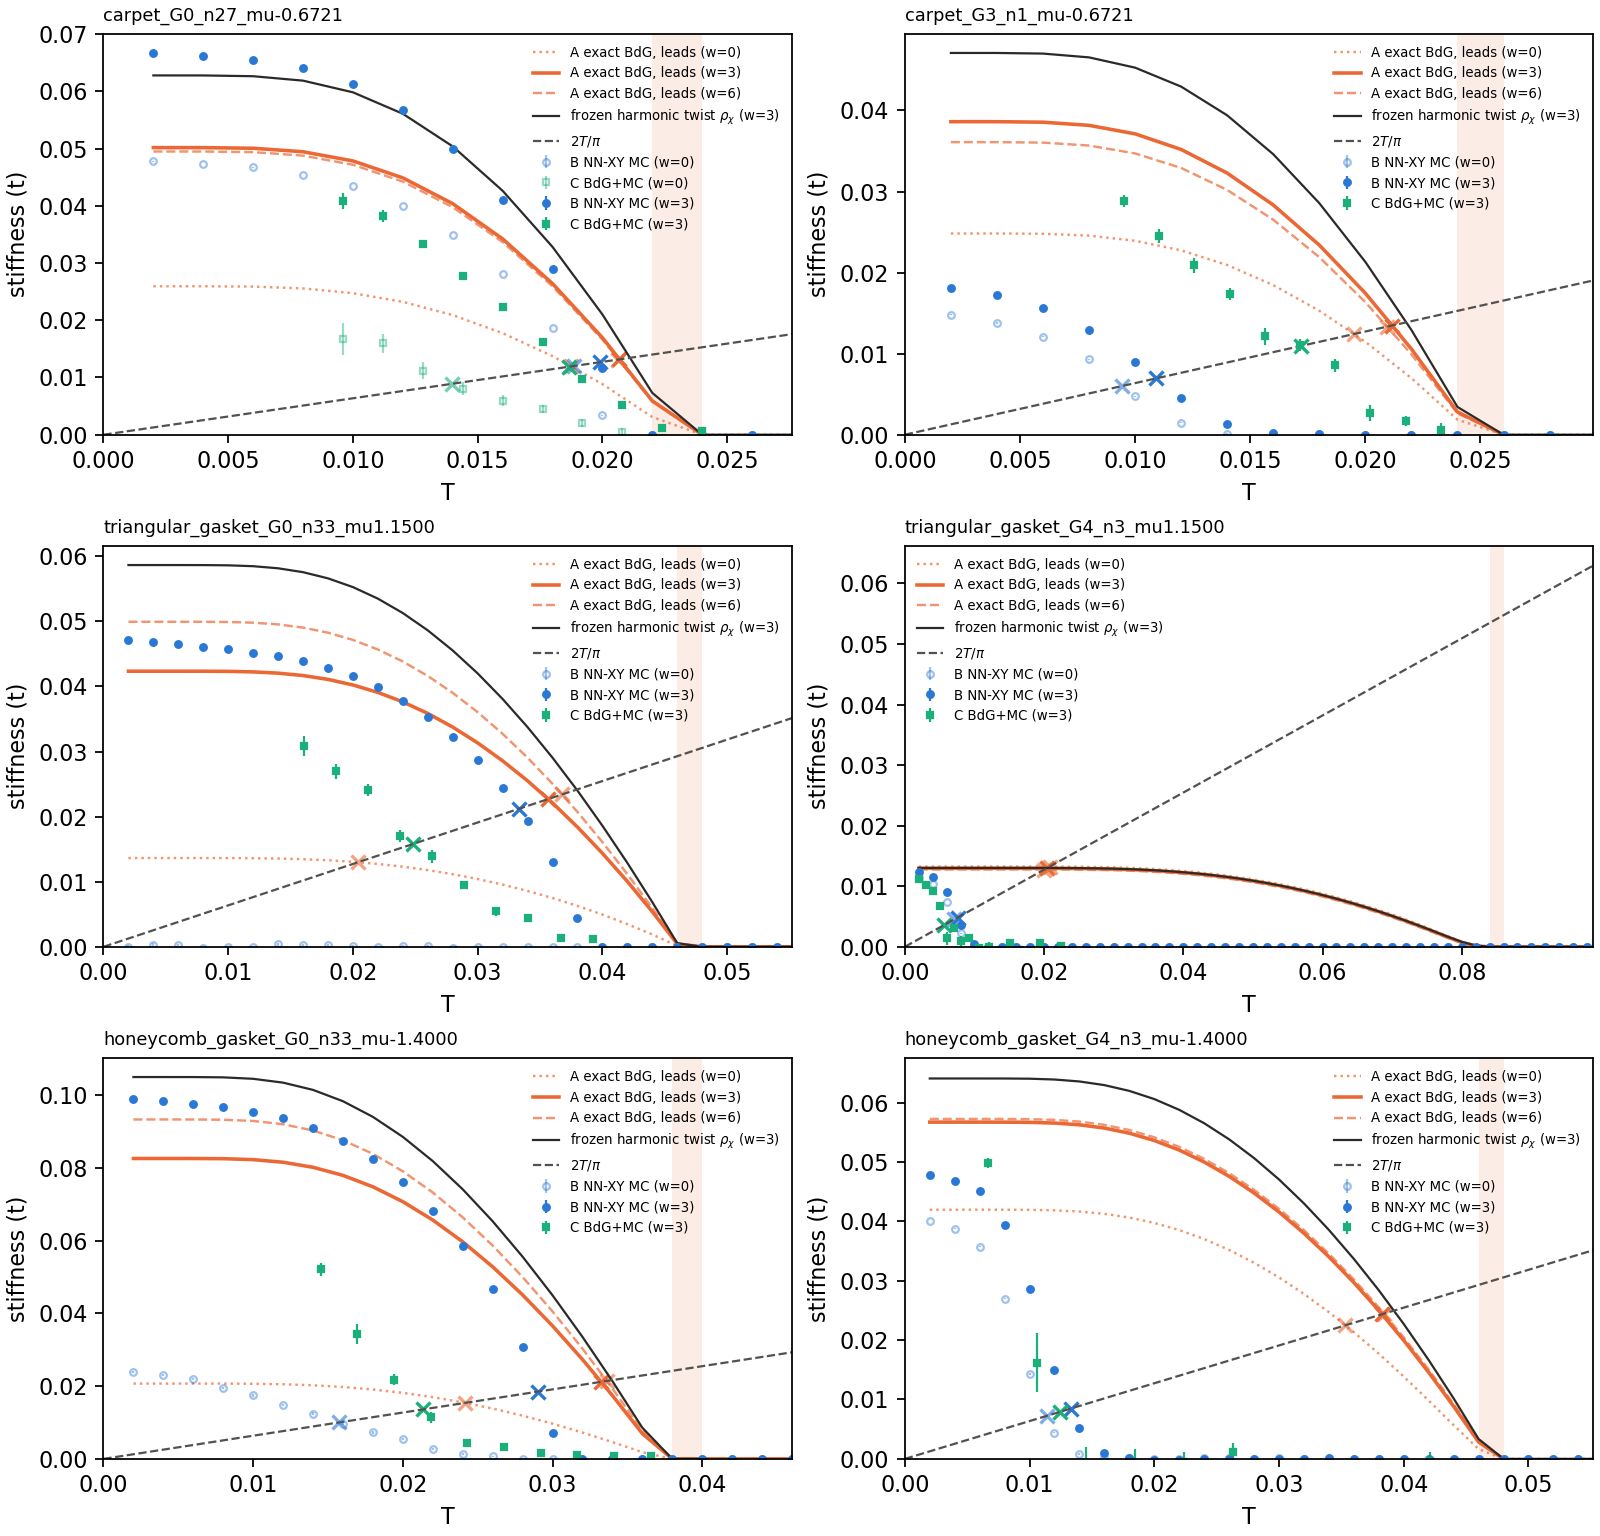
\includegraphics[width=0.95\textwidth]{tbkt_summary.png}
\caption{Two-terminal superfluid stiffness $\rho(T)$ at intermediate coupling $U=1$ across the six benchmark geometries. Curves compare Rung~A (exact self-consistent lead twist without thermal fluctuations, orange, shown for contact widths $w=0$ dotted, $w=3$ solid, and $w=6$ dashed), the frozen harmonic-twist upper bound $\rho_\chi$ at $w=3$ (black), Rung~B (nearest-neighbor XY Monte Carlo with temperature-dependent BdG couplings $J_b(T)$, blue, open markers for $w=0$ and filled markers for $w=3$), and Rung~C0 (static-path BdG Monte Carlo over amplitudes and phases at $w=3$, green). Crosses denote intersections with the BKT universal line $2T/\pi$, and the vertical shaded bands indicate the mean-field pairing temperature $\Tmf$.}
\label{fig:tbkt_summary}
\end{figure*}

The resulting temperature profiles of the two-terminal stiffness $\rho(T)$ are displayed in Fig.~\ref{fig:tbkt_summary}, and the corresponding crossover temperatures are summarized in Table~\ref{tab:u1} and compared visually in Fig.~\ref{fig:tc_comparison}. On the finitely ramified gaskets, a striking dichotomy emerges between pair formation and macroscopic phase coherence. At the mean-field level, carving the triangular lattice into a $G=4$ Sierpi\'nski gasket nearly doubles the pairing onset temperature $\Tmf$ relative to the filled triangular parent flake of identical outer dimension, while a similar, milder enhancement occurs on the honeycomb gasket. Inspection of the normal-state tight-binding spectrum confirms that this enhancement is driven by spectral compression~\cite{Iliasov2019,Iliasov2020,Iliasov2024,Canyellas2026dwave}: although the strict degeneracy of individual levels near the Fermi energy remains modest (at most threefold on the triangular gasket and sixfold on the honeycomb gasket within the pairing window), recursive decimation piles nearly one-fifth of all single-particle states of the triangular gasket into a narrow spectral cluster just outside the gap edge at $\varepsilon - \mu \approx +0.15$. This reservoir of localized and quasi-flat states amplifies the pairing susceptibility and stabilizes a robust local gap amplitude $|\Delta_i|$ up to temperatures well above the parent crystal's transition.

\begin{figure}[htbp]
\centering
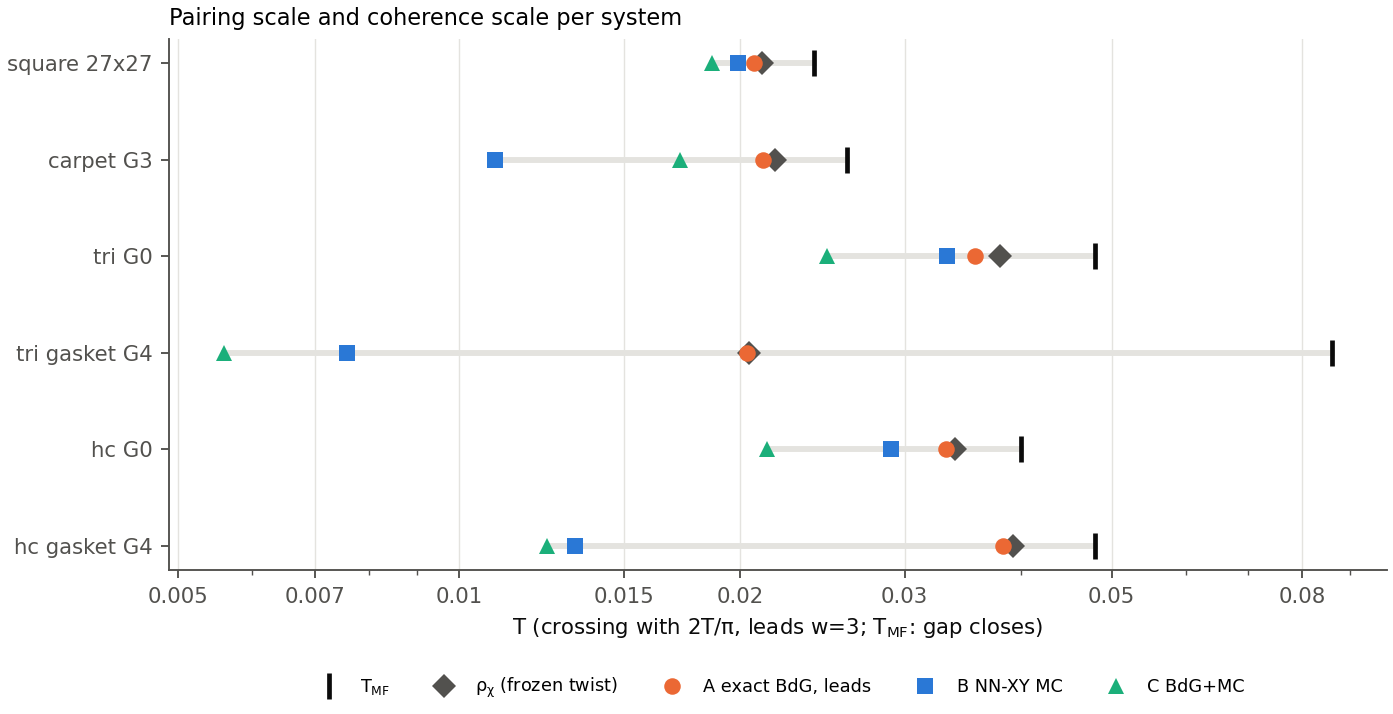
\includegraphics[width=0.95\columnwidth]{tc_comparison.png}
\caption{Comparison of the characteristic temperature scales at $U=1$ ($w=3$) across the six systems: mean-field pairing onset $\Tmf$, harmonic upper bound $T_\chi$, no-fluctuation BdG lead-twist crossover $T_A$ (Rung~A), BdG-coupled XY crossover $T_B$ (Rung~B), and full static-path BdG Monte Carlo crossover $T_{C0}$ (Rung~C0). On finitely ramified gaskets, enhanced pairing $\Tmf$ is accompanied by a severe collapse of the phase-coherence scales $T_B$ and $T_{C0}$.}
\label{fig:tc_comparison}
\end{figure}

Yet the very geometric bottlenecks responsible for this spectral localization prove destructive to global phase rigidity. On the triangular gasket, every elementary triangular block communicates with neighboring sub-blocks solely through single corner articulation vertices of coordination $z=4$, while large internal lacunae interrupt direct current paths across the interior. Even before thermal phase fluctuations are introduced, the zero-temperature mean-field two-terminal stiffness $\rlead$ (Rung~A) is severely reduced on the triangular gasket compared with its filled parent, pulling the no-fluctuation crossing $T_A$ down to less than a quarter of $\Tmf$. Once thermal fluctuations are switched on in Rung~B, the phase stiffness collapses at far lower temperatures: on the triangular gasket, the XY crossover $T_B$ drops to roughly one-eleventh of $\Tmf$ and less than a quarter of the filled triangular parent's $T_B$. Put differently, the cost of thermal phase fluctuations—measured by the ratio $T_A / T_B$—is nearly a factor of three on both the triangular and honeycomb gaskets, whereas on the filled square, triangular, and honeycomb parents $T_A / T_B$ remains close to unity ($1.0\text{--}1.1$). Fractal geometry on finitely ramified gaskets thus opens a vast temperature window, spanning nearly an order of magnitude below $\Tmf$, in which electrons are tightly bound into local Cooper pairs that lack global phase coherence.

\begin{table}[htbp]
\caption{Sensitivity of the $U=1$ ($w=3$) phase-coherence crossover temperatures to the transition criterion across Rungs~B, P, and C0. For each method we list the default universal-jump crossing (`coded', $\rho = 2T/\pi$), the sheet-rescaled crossing (`sheet', $\rho = 2T/(\pi s)$, where $s = \sigma_{\mathrm{parent}}\,g_0/g_{0,\mathrm{parent}}$ incorporates the geometric aspect factor $\sigma = 1, \sqrt{3}, 1/\sqrt{3}$ of the parent square, triangular, and honeycomb lattices), and the normalization-independent half-stiffness temperature $T_{50}$ where $\rho(T)$ falls to half of its no-fluctuation reference ($\rho_{\mathrm{harm}}$ for B, $\rho_A$ for P and C0). Statistical uncertainties are $\le 10^{-4}$ for B and P and $1\text{--}7\times 10^{-4}$ for C0.}
\label{tab:criteria}
\begin{ruledtabular}
\begin{tabular}{lcccc}
System & $s$ & $T_B$ & $T_P$ & $T_{C0}$ \\
 & & \multicolumn{3}{c}{(coded / sheet / $T_{50}$)} \\
\hline
Triangular $G=4$ & 0.43 & .0076 / .0061 / .0070 & .0060 / .0049 / .0052 & .0056 / .0049 / .0051 \\
Honeycomb $G=4$ & 0.14 & .0133 / .0084 / .0106 & .0086 / .0063 / .0062 & .0124 / .0082 / .0092 \\
Carpet $G=3$ & 0.41 & .0109 / .0081 / .0099 & .0104 / .0072 / \phantom{.00}--\phantom{0} & .0172 / .0129 / .0146 \\
Triangular $G_0$ & 1.73 & .0333 / .0359 / .0361 & -- & .0248 / .0284 / .0230 \\
Honeycomb $G_0$ & 0.58 & .0290 / .0280 / .0285 & -- & .0214 / .0195 / .0164 \\
Square ($G_0$) & 1.00 & .0199 / .0199 / .0202 & -- & .0187 / .0187 / .0188 \\
\end{tabular}
\end{ruledtabular}
\end{table}

\begin{figure*}[htbp]
\centering
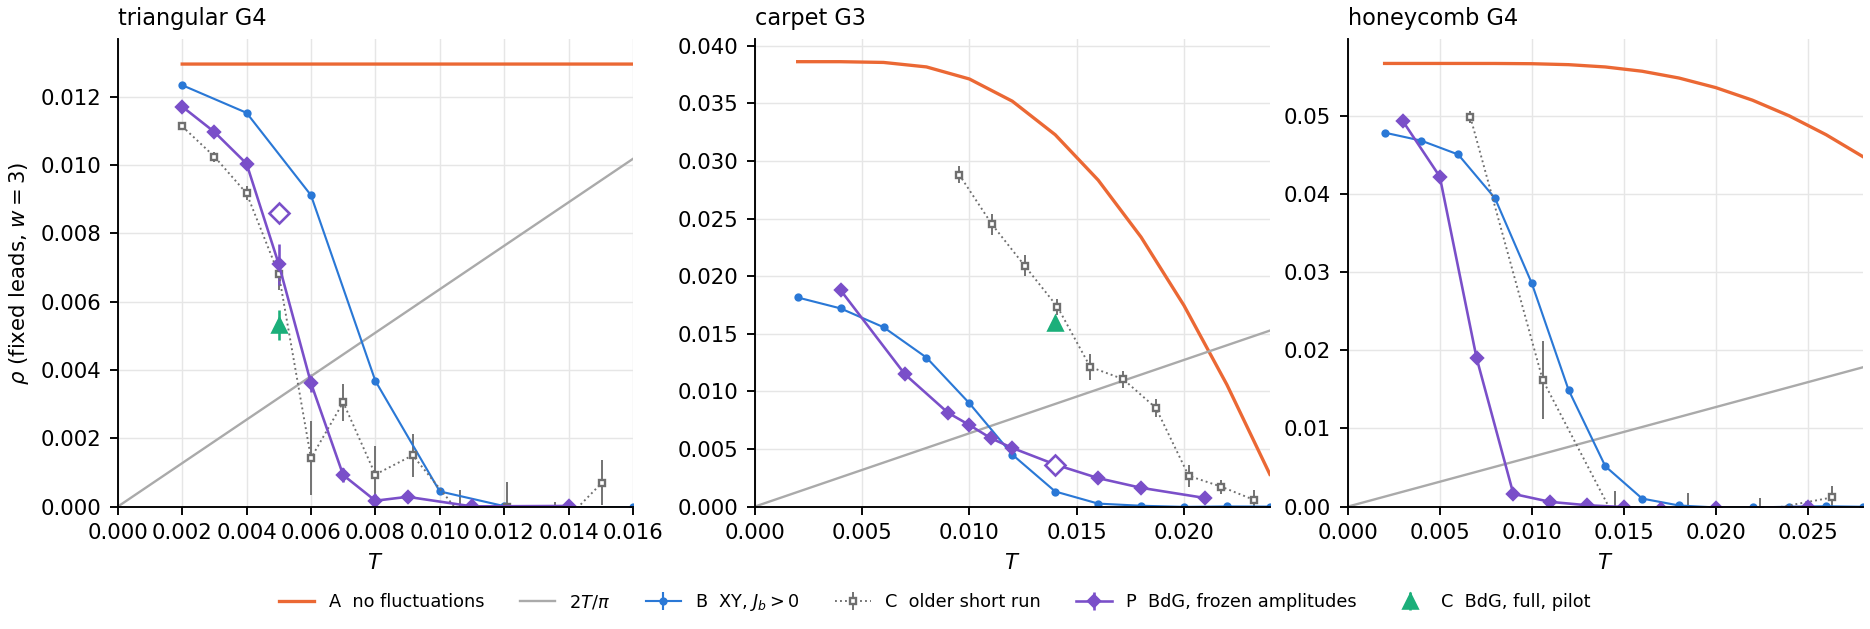
\includegraphics[width=0.95\textwidth]{u1_helicity_ladder.png}
\caption{The four-rung stiffness hierarchy at $U=1$ ($w=3$) on the three fractal flakes: triangular gasket $G=4$ (left), Sierpi\'nski carpet $G=3$ (center), and honeycomb gasket $G=4$ (right). Shown are Rung~A (orange), Rung~B (blue circles), Rung~P (exact static-path BdG phase functional with frozen amplitudes, purple filled diamonds for 10-temperature production runs and open diamond for hot/cold equilibration pilots), Rung~C0 (short unit-mass Cartesian BdG HMC, grey open squares), and the kernel-preconditioned Rung~C pilot (green triangle). The dashed grey line marks the BKT criterion $2T/\pi$.}
\label{fig:u1_helicity_ladder}
\end{figure*}

Ascending from the effective XY model (Rung~B) to the microscopic fermionic functional (Rungs~P and~C, Fig.~\ref{fig:u1_helicity_ladder}) tests whether this collapse is an artifact of the local spin mapping. On both gaskets, the frozen-amplitude BdG functional (Rung~P) and the full amplitude-and-phase BdG Monte Carlo (Rung~C0) closely track the XY crossover $T_B$, confirming that the suppression of the transition temperature by an order of magnitude relative to $\Tmf$ is a genuine property of the interacting electron system. At the same time, Rung~C0 demonstrates that the finite gasket flake does achieve a true phase-coherent condensate at sufficiently low temperatures ($T \ll T_C$). Because the pinned contacts break global $\mathrm{U}(1)$ invariance and fix the overall phase gauge, the spatial average of the thermally averaged complex order parameter, $\overline{|\langle \Delta_i \rangle|}$, serves as a direct measure of the coherent superconducting gap. As shown in Table~\ref{tab:u1}, at the lowest simulated temperatures this coherent gap recovers nearly the full mean-field amplitude (reaching nearly $90\%$ of the mean-field value on the triangular gasket and $98\%$ on the square lattice). By contrast, the unaveraged modulus $\langle |\Delta_i| \rangle$ is contaminated by incoherent Gaussian amplitude fluctuations of thermal variance $\sim \sqrt{UT}$ from the quartic Hubbard-Stratonovich weight $\exp(-|\Delta_i|^2/UT)$, causing $\langle |\Delta_i| \rangle$ to remain large—and even grow with temperature—well above $\Tmf$.

Table~\ref{tab:criteria} further verifies that these conclusions do not depend on how the BKT criterion is normalized on a non-Euclidean graph. Because a fractal lacks a conventional two-dimensional sheet thickness, one may locate the crossover either via the conductance-normalized universal jump $\rho(T) = 2T/\pi$ (`coded'), via a sheet-rescaled line $\rho(T) = 2T/(\pi s)$ that inherits the geometric aspect ratio $\sigma$ of the parent Bravais lattice rescaled by the conductance ratio $g_0/g_{0,\mathrm{parent}}$ (`sheet'), or via the purely internal half-stiffness criterion $T_{50}$ where $\rho(T)$ drops to half of its no-fluctuation baseline. Across all three definitions, the relative hierarchy of methods and the dramatic suppression of gasket coherence relative to the parent crystals remain invariant.

The infinitely ramified Sierpi\'nski carpet ($G=3$) behaves in a qualitatively different manner from the finitely ramified gaskets (Fig.~\ref{fig:u1_helicity_ladder}, center panel). Its mean-field pairing temperature $\Tmf$ is virtually identical to that of the $27\times 27$ square parent~\cite{Iliasov2024}, as the carpet lacks the sharp articulation bottlenecks that generate localized spectral clusters. However, its Rung~B XY crossing falls to about half of $T_A$, whereas the full fermionic Monte Carlo (Rung~C0) recovers a much higher stiffness, crossing $2T/\pi$ at $T_{C0} \approx 1.58\,T_B$. Even more remarkably, in our single-temperature equilibration pilot at $T=0.014$, freeing the pairing amplitudes from Rung~P to Rung~C increases the two-terminal stiffness on the carpet by more than a factor of four, whereas on the triangular gasket at $T=0.005$ freeing the amplitudes slightly reduces the stiffness. To understand why the nearest-neighbor XY mapping succeeds on the gaskets yet fails on the carpet and filled lattices—and why contact geometry plays a decisive role at $U=1$—we must examine the hierarchy of microscopic length scales.

%----------------------------------------------------------------------
\subsection{Microscopic length scales and Pippard nonlocality at the contacts}
\label{sec:length_scales_contacts}
%----------------------------------------------------------------------

The validity of any local phase model rests on a separation of length scales: the size of a Cooper pair must be small compared with both the geometric features of the sample and the scale over which the superconducting phase twists. From the converged self-consistent BdG solutions at $U=1$, we extract three distinct microscopic lengths (Table~\ref{tab:lengths} and Fig.~\ref{fig:length_scales}):
\begin{enumerate}
\item The root-mean-square Cooper-pair radius $\xi_{\mathrm{pair}}$, defined through the spatial second moment of the anomalous pairing correlator $F_{ij} = \langle c_{i\downarrow} c_{j\uparrow} \rangle$,
\begin{equation}
\xi_{\mathrm{pair}}^2 = \frac{\sum_{ij} d_{ij}^2 |F_{ij}|^2}{\sum_{ij} |F_{ij}|^2},
\label{eq:xi_pair_sec5}
\end{equation}
which automatically incorporates both conventional intraband dispersion and the multiband quantum-geometric contributions prominent in flat-band and fractal systems~\cite{PT15,CHK23,HUW23,Isk24}.
\item The phase-kernel range $\xi_K$, measuring the spatial decay of the exact site-space phase Laplacian $L = \frac{1}{4}B^T K^{(\alpha)} B$ applied to a localized point source.
\item The Ginzburg--Landau amplitude coherence length $\xi_{\mathrm{GL}}$, extracted from the spatial decay of the inverse amplitude Hessian $\partial^2 F / \partial \operatorname{Re}\Delta_i \partial \operatorname{Re}\Delta_j$.
\end{enumerate}

\begin{table}[htbp]
\caption{Microscopic superconducting length scales (in Euclidean lattice units at the lowest simulated temperature for $U=1$), locality and frustration of the phase kernel, and two-terminal contact efficiency $\rlead/\rho_\chi$ at lead width $w=3$. Listed are the rms Cooper-pair size $\xi_{\mathrm{pair}}$, phase-kernel range $\xi_K$, Ginzburg--Landau amplitude length $\xi_{\mathrm{GL}}$ (honeycomb nearest-neighbor bond length is $1/\sqrt{3}\approx 0.577$), the fraction of total phase-kernel weight carried by nearest-neighbor bonds (NN share), the percentage of bonds acquiring negative projected XY couplings $J_b < 0$, and the contact stiffness ratio $\rlead/\rho_\chi$.}
\label{tab:lengths}
\begin{ruledtabular}
\begin{tabular}{lcccccc}
System & $\xi_{\mathrm{pair}}$ & $\xi_K$ & $\xi_{\mathrm{GL}}$ & NN share & Neg.\ $J_b$ & $\rlead/\rho_\chi$ \\
\hline
Square ($G_0$) & 9.60 & 7.72 & 3.76 & 0.12 & 0\% & 0.80 \\
Carpet $G=3$ & 6.15 & 6.06 & 2.53 & 0.17 & 14--15\% & 0.82 \\
Triangular $G_0$ & 4.59 & 5.59 & 2.48 & 0.20 & 2--4\% & 0.72 \\
Triangular $G=4$ & 0.99 & 1.33 & 0.75 & 0.71 & 1.7\% & 1.00 \\
Honeycomb $G_0$ & 3.09 & 4.01 & 1.60 & 0.18 & 0.8\% & 0.79 \\
Honeycomb $G=4$ & 1.50 & 1.55 & 0.56 & 0.48 & 0.8\% & 0.89 \\
\end{tabular}
\end{ruledtabular}
\end{table}

\begin{figure*}[htbp]
\centering
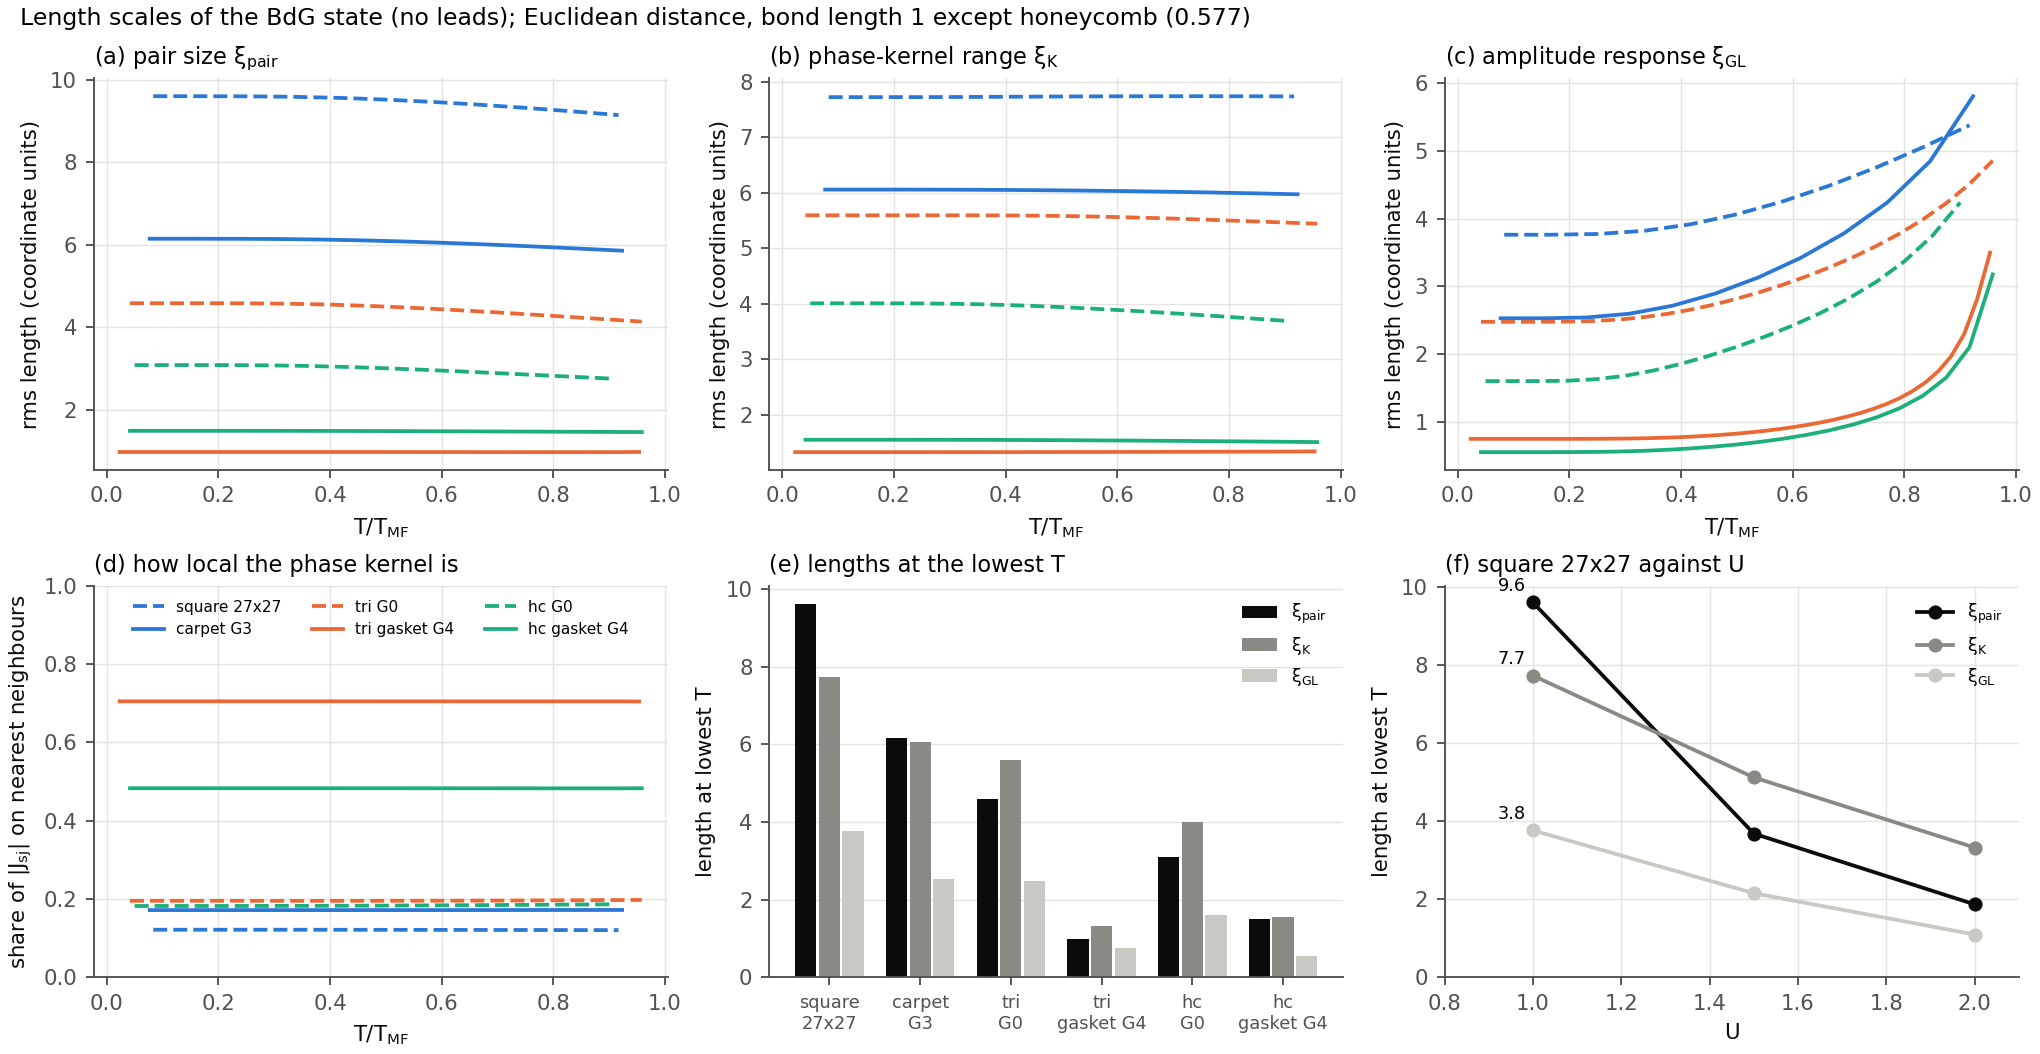
\includegraphics[width=0.92\textwidth]{length_scales.png}
\caption{Microscopic superconducting length scales extracted from the self-consistent BdG solution: rms Cooper-pair radius $\xi_{\mathrm{pair}}$, phase-kernel range $\xi_K$, and Ginzburg--Landau amplitude coherence length $\xi_{\mathrm{GL}}$ plotted as functions of reduced temperature $T/\Tmf$ at $U=1$ across the six systems, and as a function of attraction $U$ on the $27\times 27$ square lattice. On finitely ramified gaskets, fractal confinement compresses all three scales to the single-bond lattice spacing.}
\label{fig:length_scales}
\end{figure*}

\begin{figure*}[htbp]
\centering
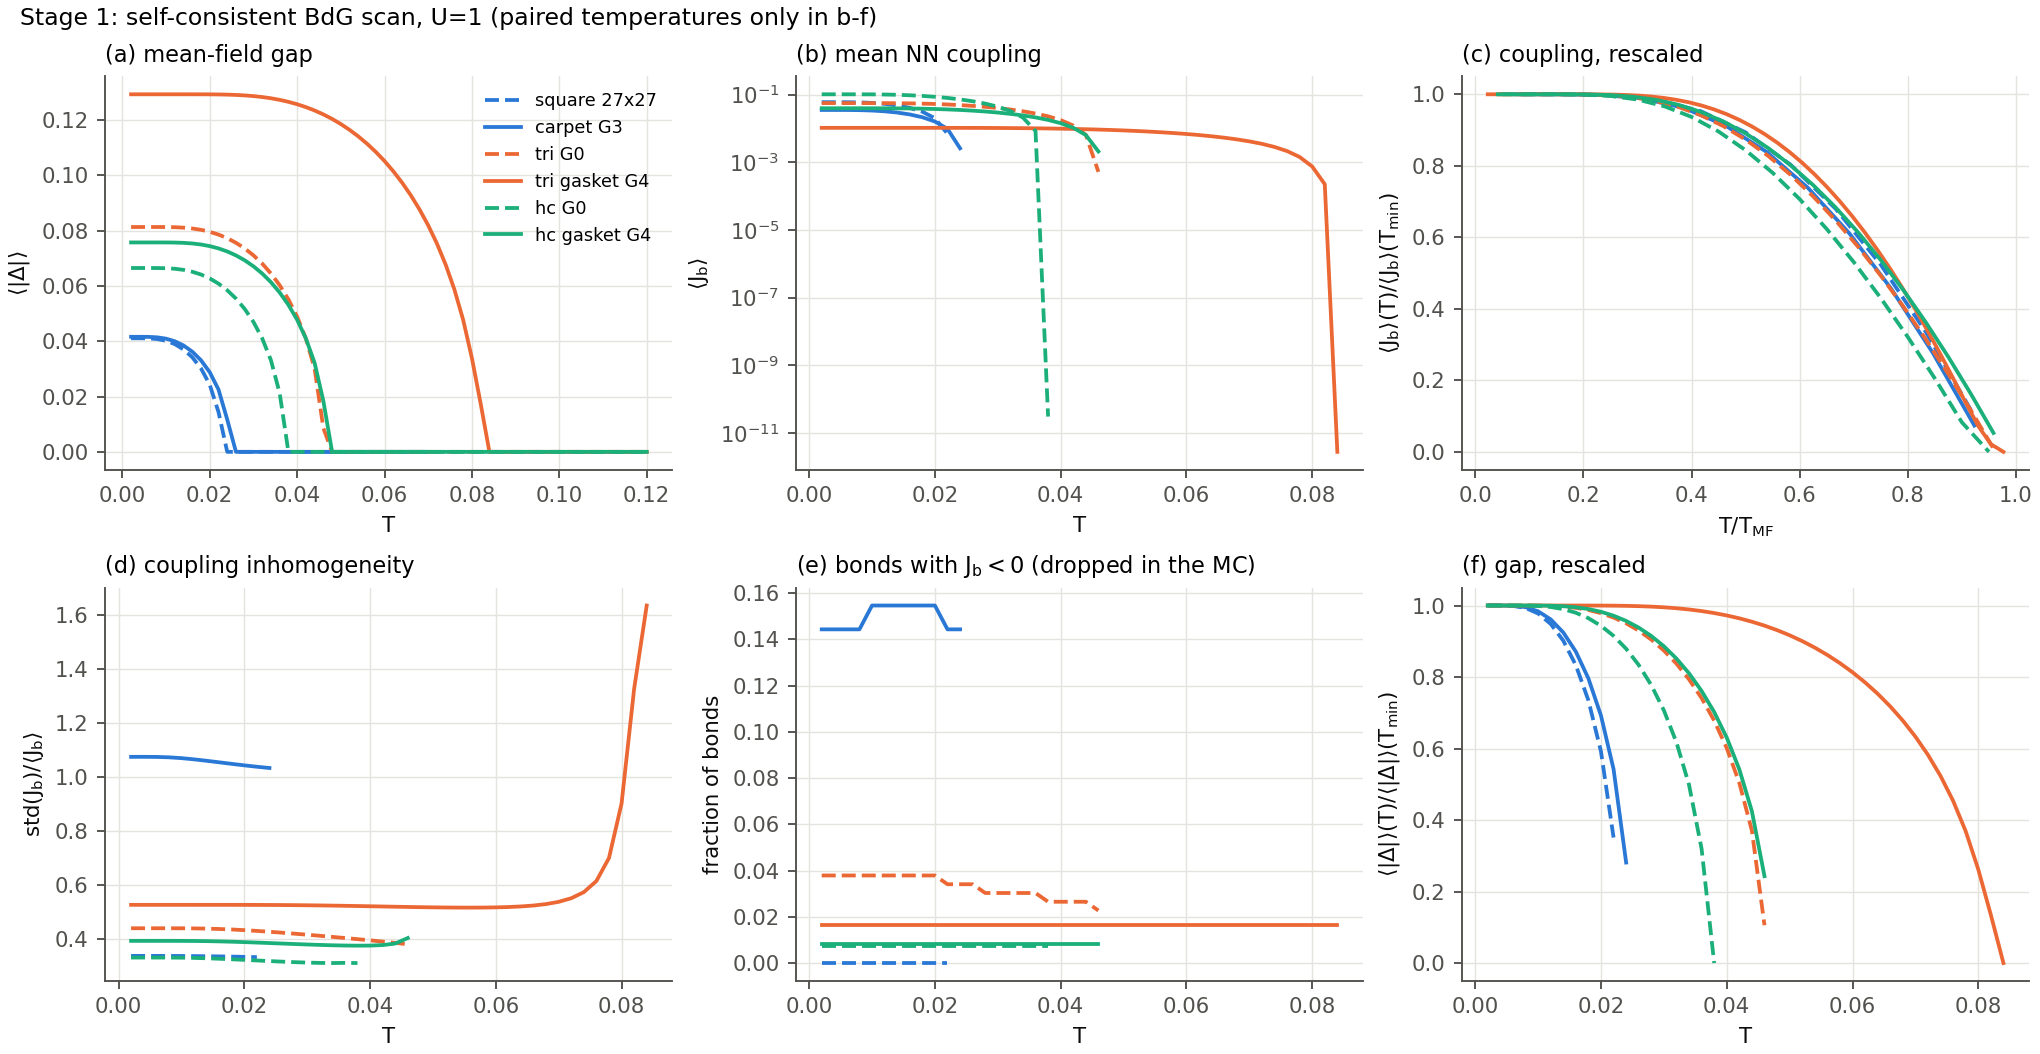
\includegraphics[width=0.92\textwidth]{stage1_couplings.png}
\caption{Temperature evolution of the Stage-1 microscopic BdG properties at $U=1$: mean pairing gap $|\Delta|$, mean positive nearest-neighbor phase coupling $\bar{J}_b$, relative spatial disorder $\mathrm{std}(J_b)/\bar{J}_b$, and fraction of negative projected couplings $J_b < 0$. The Sierpi\'nski carpet exhibits the strongest coupling inhomogeneity ($\mathrm{std}(J_b)/\bar{J}_b \approx 1.07$) and a $14\%\text{--}15\%$ share of frustrated negative bonds.}
\label{fig:stage1_couplings}
\end{figure*}

As revealed by Table~\ref{tab:lengths} and Fig.~\ref{fig:length_scales}, the six systems divide sharply into two physical regimes at $U=1$. On the filled Bravais lattices and on the Sierpi\'nski carpet, the Cooper pairs are mesoscopic objects spanning $\xi_{\mathrm{pair}} \approx 3\text{--}10$ lattice spacings, and the phase kernel $L_{ij}$ extends over a comparable range $\xi_K \approx 4\text{--}8$. Because the paramagnetic current-current correlator $K_{bb'}^{\mathrm{para}}$ couples bonds separated by up to $\xi_{\mathrm{pair}}$, less than one-fifth ($12\%\text{--}20\%$) of the total phase-kernel weight resides on nearest-neighbor bonds. On the carpet, where currents are forced to turn sharply around a hierarchy of square cutouts of size smaller than $\xi_K$, projecting this strongly nonlocal response onto nearest-neighbor bonds generates severe coupling disorder ($\mathrm{std}(J_b)/\bar{J}_b \approx 1.07$, Fig.~\ref{fig:stage1_couplings}) and drives $14\%\text{--}15\%$ of the projected couplings $J_b$ negative. Because the exact site kernel $L_{ij}$ is positive semidefinite and essentially free of negative couplings, these negative $J_b$ are an artifact of forcing a long-range kernel into a nearest-neighbor form. Dropping them to preserve vacuum stability in Rung~B removes real stiffness paths and leaves the XY network on the carpet artificially soft by a factor of $R = \rlead/\rho_{\mathrm{harm}} \approx 2.03$, explaining part of why $T_B$ falls anomalously below $T_{C0}$ on the carpet at $U=1$.

On the triangular and honeycomb gaskets, by contrast, recursive removal of internal triangles confines the electronic wave functions and compresses both the Cooper-pair size and the phase-kernel range down to a single bond length ($\xi_{\mathrm{pair}} \approx 1.0\text{--}1.5$, $\xi_{\mathrm{GL}} \approx 0.6\text{--}0.8$). As a consequence, half to nearly three-quarters ($48\%\text{--}71\%$) of the entire phase-kernel weight is concentrated directly on nearest-neighbor bonds, fewer than $2\%$ of the projected bond couplings turn negative, and the zero-temperature XY network stiffness matches the exact BdG lead-twist stiffness to within a few percent ($R = 1.00$ on the triangular gasket and $1.16$ on the honeycomb gasket).

\begin{figure*}[htbp]
\centering
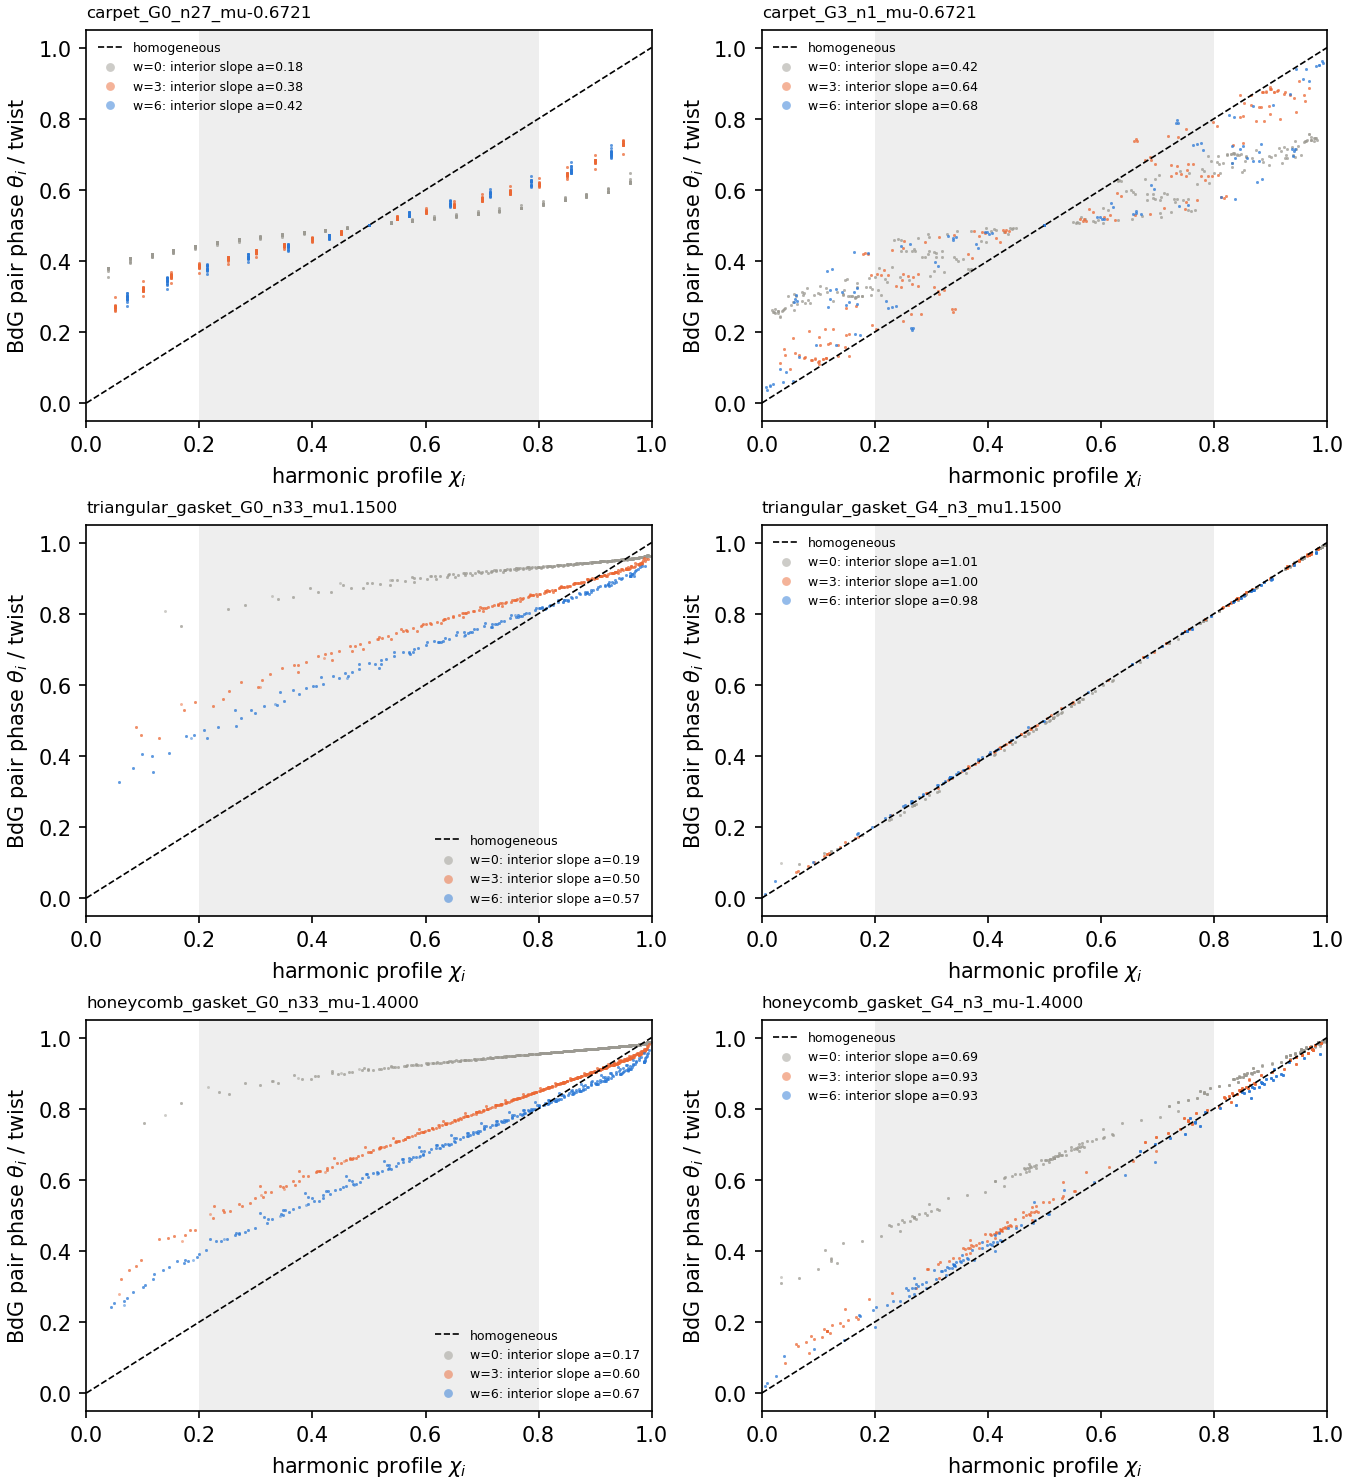
\includegraphics[width=0.92\textwidth]{lead_phase_profiles.png}
\caption{Spatial profile of the self-consistent BdG pair phase $\vartheta_i = \arg[\Delta_i(\varphi)/\Delta_i(0)]/\varphi$ in the twisted state at $U=1$ (lowest temperature) plotted against the homogeneous harmonic potential $\chi_i \in [0,1]$ for contact widths $w=0$ (single-column leads), $w=3$, and $w=6$. While the triangular gasket follows the ideal linear profile $\vartheta_i \approx \chi_i$ even for narrow contacts, the filled lattices and carpet exhibit large Pippard phase slips directly at the contact boundaries.}
\label{fig:lead_phase_profiles}
\end{figure*}

\begin{figure}[htbp]
\centering
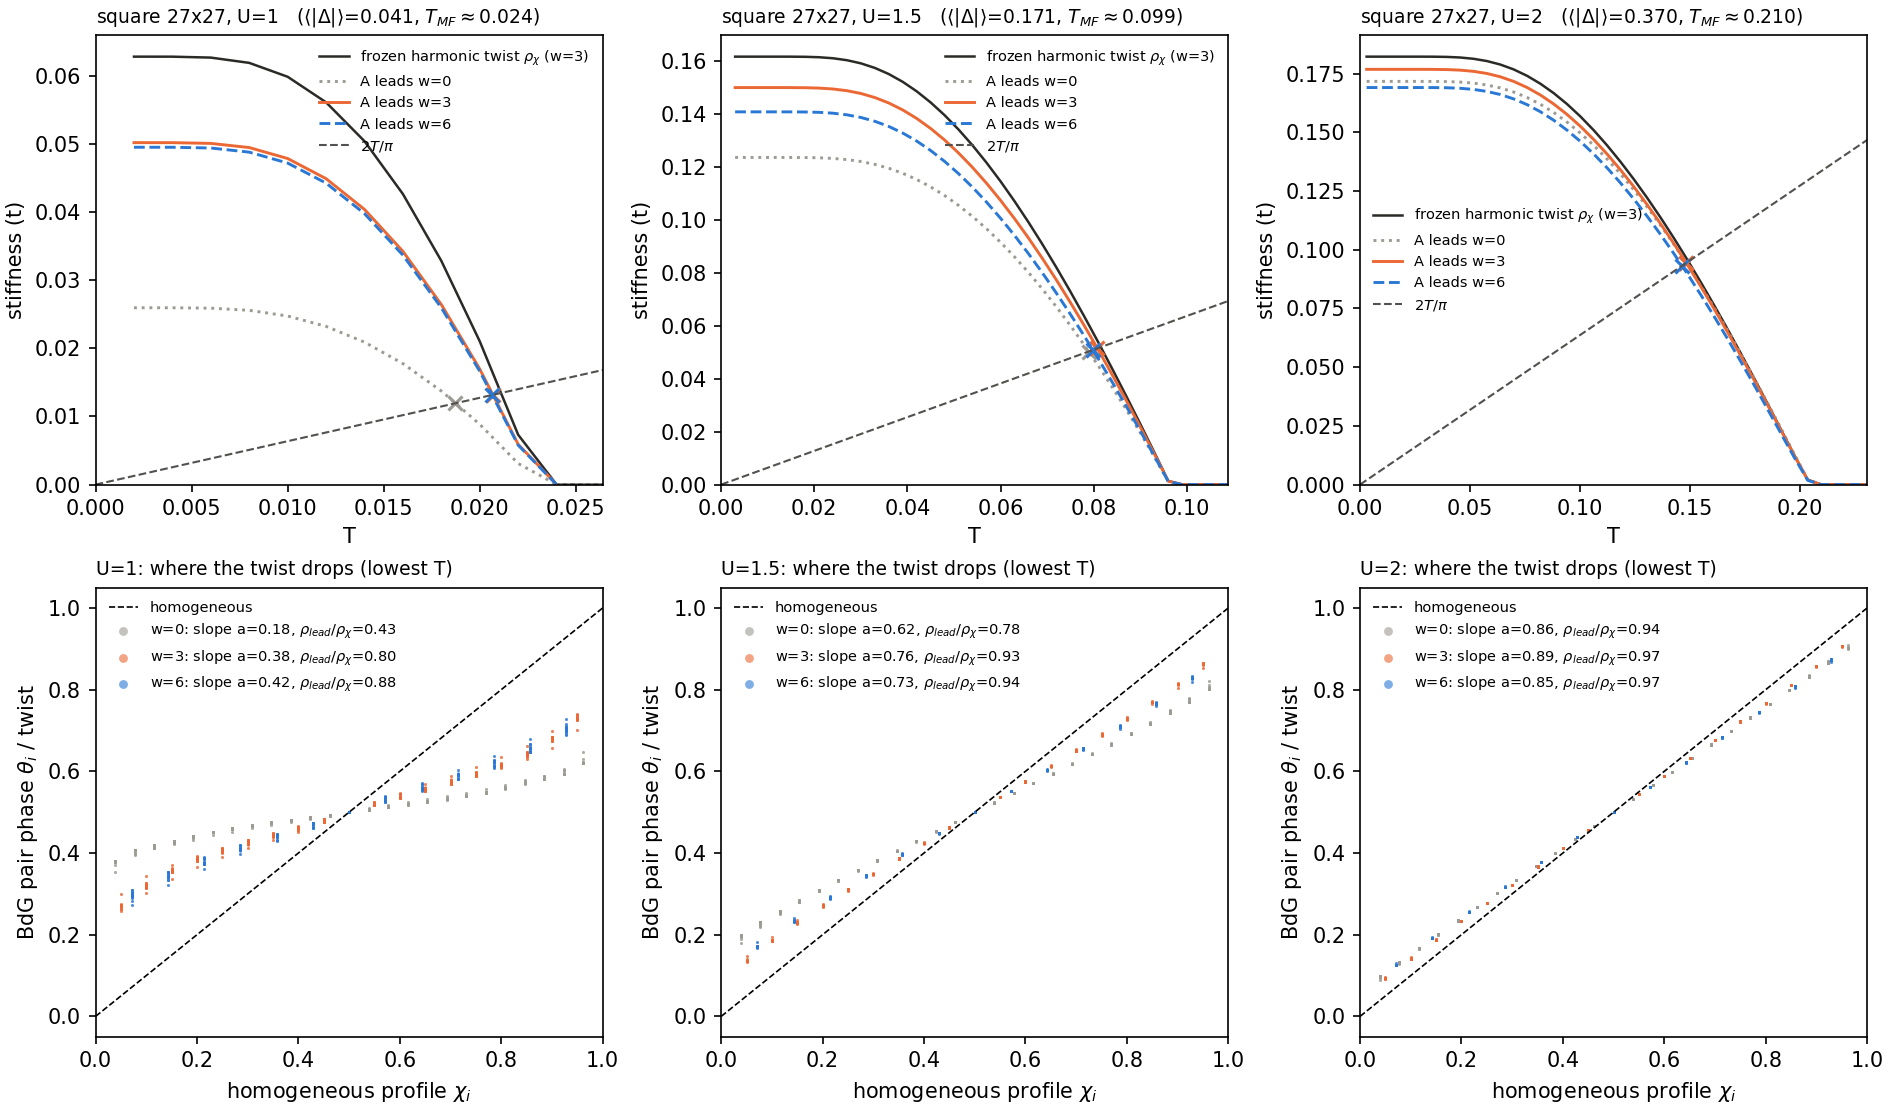
\includegraphics[width=0.95\columnwidth]{U_test_square.png}
\caption{Elimination of Pippard contact losses with increasing attractive coupling $U = 1.0, 1.5, 2.0$ on the $27\times 27$ square lattice. Top: two-terminal lead-twist stiffness $\rlead(T)$ for lead widths $w=0,3,6$ compared against the frozen harmonic upper bound $\rho_\chi$. Bottom: twisted pair-phase profile $\vartheta_i$ versus $\chi_i$. As $U$ increases to $2.0$, $\xi_{\mathrm{pair}}$ compresses from $9.6$ to $1.9$ lattice constants, eliminating boundary phase jumps and collapsing all lead widths onto $\rho_\chi$.}
\label{fig:U_test_square}
\end{figure}

\begin{figure*}[htbp]
\centering
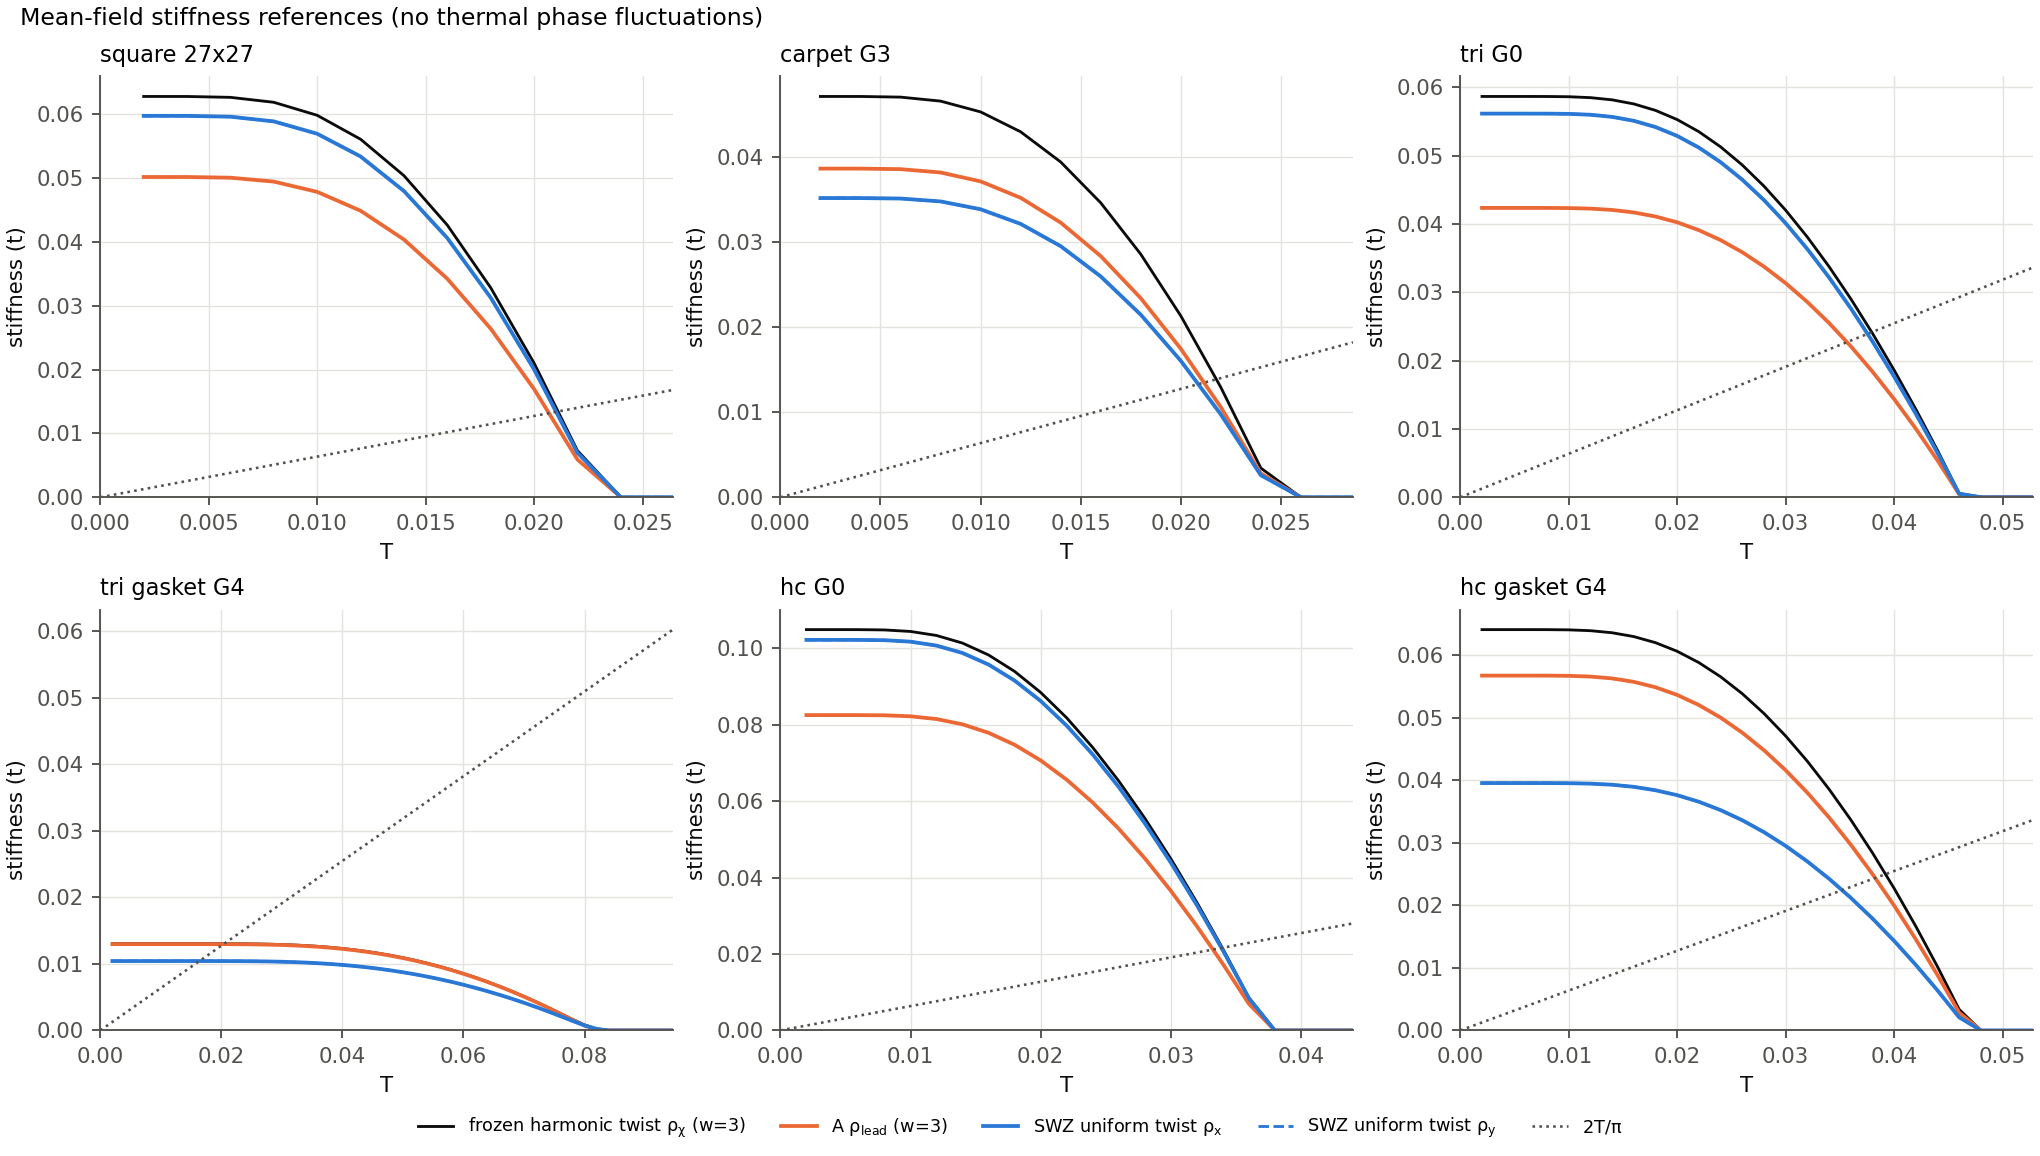
\includegraphics[width=0.92\textwidth]{stiffness_references.png}
\caption{Comparison of mean-field superfluid stiffness definitions at $U=1$ ($w=3$): uniform-twist Scalapino--White--Zhang (SWZ) weights $\rho_x, \rho_y$, frozen harmonic-twist stiffness $\rho_\chi$, self-consistent two-terminal lead-twist stiffness $\rlead$ (Rung~A), and the BKT line $2T/\pi$. On all three fractals, the uniform-twist SWZ estimator lies below $\rlead$ because supercurrents must deflect around internal lacunae rather than follow a uniform spatial gradient.}
\label{fig:stiffness_references}
\end{figure*}

This dichotomy in $\xi_{\mathrm{pair}}$ has an immediate physical consequence for two-terminal transport measurements: Pippard nonlocality at the contacts (Figs.~\ref{fig:lead_phase_profiles} and~\ref{fig:U_test_square}). In a two-terminal setup, the external reservoir pins the pair phase $\arg\Delta_i$ only on a boundary slab of depth $w$, whereas Bogoliubov quasiparticles sample the pairing field averaged over a coherence volume of radius $\xi_{\mathrm{pair}}$. When the contact is narrower than the pair size ($w \lesssim \xi_{\mathrm{pair}}$), a sharp jump of the pair phase across the single row of bonds joining the lead to the interior barely perturbs the nonlocal fermionic free energy. As shown in Fig.~\ref{fig:lead_phase_profiles}, on the $27\times 27$ square lattice with single-column leads ($w=0$), roughly $36\%$ of the entire imposed phase twist $\varphi$ drops abruptly across the single bond adjacent to each contact, leaving the interior under-twisted and depressing the measured two-terminal stiffness $\rlead$ to a fraction ($0.25\text{--}0.55$) of the bulk harmonic-twist reference $\rho_\chi$. Even at $w=3$, contact slip reduces $\rlead/\rho_\chi$ to $0.72\text{--}0.82$ on the filled lattices and the carpet (Table~\ref{tab:lengths}). On the triangular gasket, by contrast, because $\xi_{\mathrm{pair}} \approx 1$ is already at the lattice scale, the twisted pair phase follows the harmonic profile $\chi_i$ faithfully across the entire sample ($\rlead/\rho_\chi = 1.00$) with zero contact drop even for single-bond leads.

Figure~\ref{fig:stiffness_references} also clarifies why the conventional uniform-twist Scalapino--White--Zhang (SWZ) superfluid weight~\cite{SWZ93}, which applies a spatially uniform Peierls vector potential across all bonds, is inappropriate as a bulk reference on perforated fractal graphs. On a homogeneous Bravais lattice, a uniform gradient satisfies current conservation everywhere and $\rho_{\mathrm{SWZ}}$ provides the exact bulk ceiling above the contact-limited $\rlead$. On a fractal, however, an imposed uniform phase gradient drives currents straight into the open walls of internal lacunae; enforcing current conservation around the holes requires non-uniform local phase adjustments that are absent from the uniform-twist SWZ definition, causing $\rho_{\mathrm{SWZ}}$ to fall unphysically below the true two-terminal stiffness $\rlead$ on all three fractals. The proper upper bound on any perforated graph is instead $\rho_\chi$, the BdG bond Hessian evaluated on the harmonic potential $\chi_i$ that automatically routes current around every geometric hole.

\begin{table*}[htbp]
\caption{Interaction scan ($U=1$ versus $U=2$) at fixed electron filling and lowest temperature, computed from the Schur complement of the exact site-phase kernel $K_{ij} = \partial^2 F/\partial\theta_i\partial\theta_j$. Listed are the mean-field pairing scale $\Tmf$ (upper bound on the coarse scan grid), the relative stiffness scale $T_\times/\Tmf$ where $\rho_{\mathrm{harm}}$ crosses $2T/\pi$, the ratio $a_0/\sqrt{UT_\times}$ of the mean-field gap to the thermal amplitude noise at $T_\times$, the count of negative projected nearest-neighbor bonds $J_b < 0$, the exact two-terminal kernel stiffness $\rho_K(w)$ across contact widths $w=0,1,3,6$, the contact efficiency $\rho_K/\rho_\chi$ at $w=1$, and the stiffness scale ratio $R = \rho_K/\rho_{\mathrm{harm}}$ at $w=1$.}
\label{tab:uscan}
\begin{ruledtabular}
\begin{tabular}{lccccccccc}
System & $U$ & $\Tmf$ & $T_\times/\Tmf$ & $a_0/\sqrt{UT_\times}$ & Neg.\ $J_b$ & $\rho_K(w=0 / 1 / 3 / 6)$ & $\rho_K/\rho_\chi$ ($w=1$) & $R$ ($w=1$) \\
\hline
Triangular $G=4$ & 1.0 & 0.084 & 0.24 & 0.91 & 12 / 729 & .0133 / .0135 / .0130 / .0128 & 0.99 & 1.01 \\
Triangular $G=4$ & 2.0 & 0.228 & 0.31 & 1.01 & \phantom{0}6 / 729 & .0460 / .0465 / .0457 / .0459 & 0.99 & 1.03 \\
Honeycomb $G=4$ & 2.0 & 0.193 & 0.59 & 0.61 & \phantom{0}0 / 729 & .1025 / .1061 / .1063 / .1073 & 0.96 & 1.15 \\
Carpet $G=3$ & 2.0 & 0.211 & 0.69 & 0.56 & \phantom{0}0 / 776 & .1512 / .1530 / .1538 / .1526 & 0.92 & 1.01 \\
Square ($G_0$) & 1.0 & 0.024 & 0.88 & 0.13 & \phantom{0}0 / 1404 & .0259 / .0396 / .0502 / .0495 & 0.64 & 0.68 \\
Square ($G_0$) & 2.0 & 0.211 & 0.71 & 0.52 & \phantom{0}0 / 1404 & .1703 / .1774 / .1751 / .1672 & 0.97 & 0.95 \\
\end{tabular}
\end{ruledtabular}
\end{table*}

To benchmark the four-rung hierarchy across all geometries without contact artifacts or truncated negative bonds, we exploit the exact Schur-complement identity of Eq.~\eqref{eq:schur_complement}: integrating out the free interior sites from the exact site-phase kernel $K_{ij} = \partial^2 F/\partial\theta_i\partial\theta_j$ reproduces the self-consistent Rung~A stiffness $\rlead(w)$ to four significant digits at any lead width $w$ without requiring new self-consistent solves. Scanning the attraction strength $U$ at fixed electron filling (Table~\ref{tab:uscan} and Fig.~\ref{fig:U_test_square}) demonstrates that increasing the attraction to $U=2$ compresses the Cooper-pair radius on the square lattice from $\xi_{\mathrm{pair}} = 9.6$ down to $1.9$ lattice spacings. As a result, at $U=2$ all negative projected couplings vanish on the carpet and honeycomb gasket (and drop below $1\%$ of bonds on the triangular gasket), the linear-response stiffness scale ratio settles near unity across every geometry ($R \in [0.95, 1.15]$ at $w=1$), and the two-terminal stiffness becomes independent of contact width to within $2\%\text{--}5\%$ between $w=0$ and $w=6$. Choosing thin leads of width $w=1$ at $U=2$ thus eliminates Pippard contact resistance while avoiding the pinning of a third of the flake interior that occurs at $w=3$.

Two technical features of the strong-coupling regime are essential for numerical reproducibility. First, because the on-site attractive Hartree shift $-U n_{i\bar{\sigma}}$ makes the compressibility $n(\mu)$ extremely steep near the spectral clusters of the gaskets, holding $\mu$ fixed at $U=2$ causes abrupt density jumps out of the paired window; we therefore root-find $\mu(T)$ at every temperature to hold the electron filling $\langle n \rangle$ strictly fixed at its $U=1$ benchmark value ($1.4229$ on triangular gaskets, $0.6651$ on honeycomb gaskets, $0.8996$ on the carpet, $1.4519$ on triangular $G_0$, $0.7200$ on honeycomb $G_0$, and $0.8750$ on the square). Second, because a weak-gap initialization on the triangular gaskets at $U=2$ can get trapped in a metastable unpaired normal state of higher grand potential, all self-consistent trajectories are initialized from a strong pairing branch ($|\Delta_{\mathrm{init}}| = 1.0$) and guarded against Anderson-mixing collapse to the normal fixed point.

%----------------------------------------------------------------------
\subsection{Strong coupling (\texorpdfstring{$U=2$}{U=2}): Validity of the XY mapping and generation scaling}
\label{sec:u2_campaign}
%----------------------------------------------------------------------

Table~\ref{tab:u2} and Fig.~\ref{fig:u2_ladder} present the central results of our second production campaign, comparing all four rungs (A, B, P, and C) at $U=2$ and contact width $w=1$ across ten lattices spanning three fractal families, three gasket generations ($G=3,4,5$), and their filled parent flakes.

\begin{table*}[htbp]
\caption{Complete four-rung fixed-lead benchmark at strong coupling $U=2$, lead width $w=1$, and fixed electron filling across ten fractal and parent lattices. Listed are the zero-temperature mean-field two-terminal stiffness $\rho_A(T\to 0)$, the mean-field pairing scale $\Tmf$, the BKT crossover temperatures $T_A$ (exact BdG lead twist), $T_B$ (BdG-coupled nearest-neighbor XY Monte Carlo), $T_P$ (frozen-amplitude static-path BdG HMC), and $T_C$ (full amplitude-and-phase static-path BdG HMC) under the universal jump criterion $\rho(T) = 2T/\pi$, together with the methodological comparison ratios $T_P/T_B$ and $T_C/T_B$. Statistical uncertainties in the last digit are given in parentheses (where omitted, errors are below $5\times 10^{-5}$).}
\label{tab:u2}
\begin{ruledtabular}
\begin{tabular}{lcccccccc}
System & $\rho_A(T\!\to\!0)$ & $\Tmf$ & $T_A$ & $T_B$ & $T_P$ & $T_C$ & $T_P/T_B$ & $T_C/T_B$ \\
\hline
Triangular gasket $G=3$ & 0.0421 & -- & 0.0659 & 0.0305 & 0.0247(1) & 0.0274(1) & 0.81 & 0.90 \\
Triangular gasket $G=4$ & 0.0465 & 0.21--0.23 & 0.0726 & 0.0259 & 0.0228(2) & 0.0224(1) & 0.88 & 0.86 \\
Triangular gasket $G=5$ & -- & -- & -- & 0.0198 & $<0.0245$ & -- & -- & -- \\
Honeycomb gasket $G=3$ & 0.1017 & -- & 0.1186 & 0.0354(1) & 0.0317(2) & 0.0367(1) & 0.90 & 1.04 \\
Honeycomb gasket $G=4$ & 0.1061 & 0.18--0.19 & 0.1209 & 0.0255(1) & 0.0260(2) & 0.0266(4) & 1.02 & 1.04 \\
Honeycomb gasket $G=5$ & -- & -- & -- & 0.0170(1) & -- & -- & -- & -- \\
Sierpi\'nski carpet $G=3$ & 0.1530 & 0.19--0.21 & 0.1440 & 0.0832(1) & 0.0498(1) & 0.0635(4) & 0.60 & 0.76 \\
Square parent ($27\times 27$) & 0.1774 & 0.19--0.20 & 0.1465 & 0.1204 & 0.0585(2) & 0.0752(2) & 0.49 & 0.62 \\
Triangular parent $G_0$ & 0.0821 & 0.21--0.23 & 0.1127 & 0.0876(1) & 0.0574(1) & 0.0649(4) & 0.66 & 0.74 \\
Honeycomb parent $G_0$ & 0.1315 & 0.19--0.21 & 0.1327 & 0.0806(1) & 0.0458(3) & -- & 0.57 & -- \\
\end{tabular}
\end{ruledtabular}
\end{table*}

\begin{figure*}[htbp]
\centering
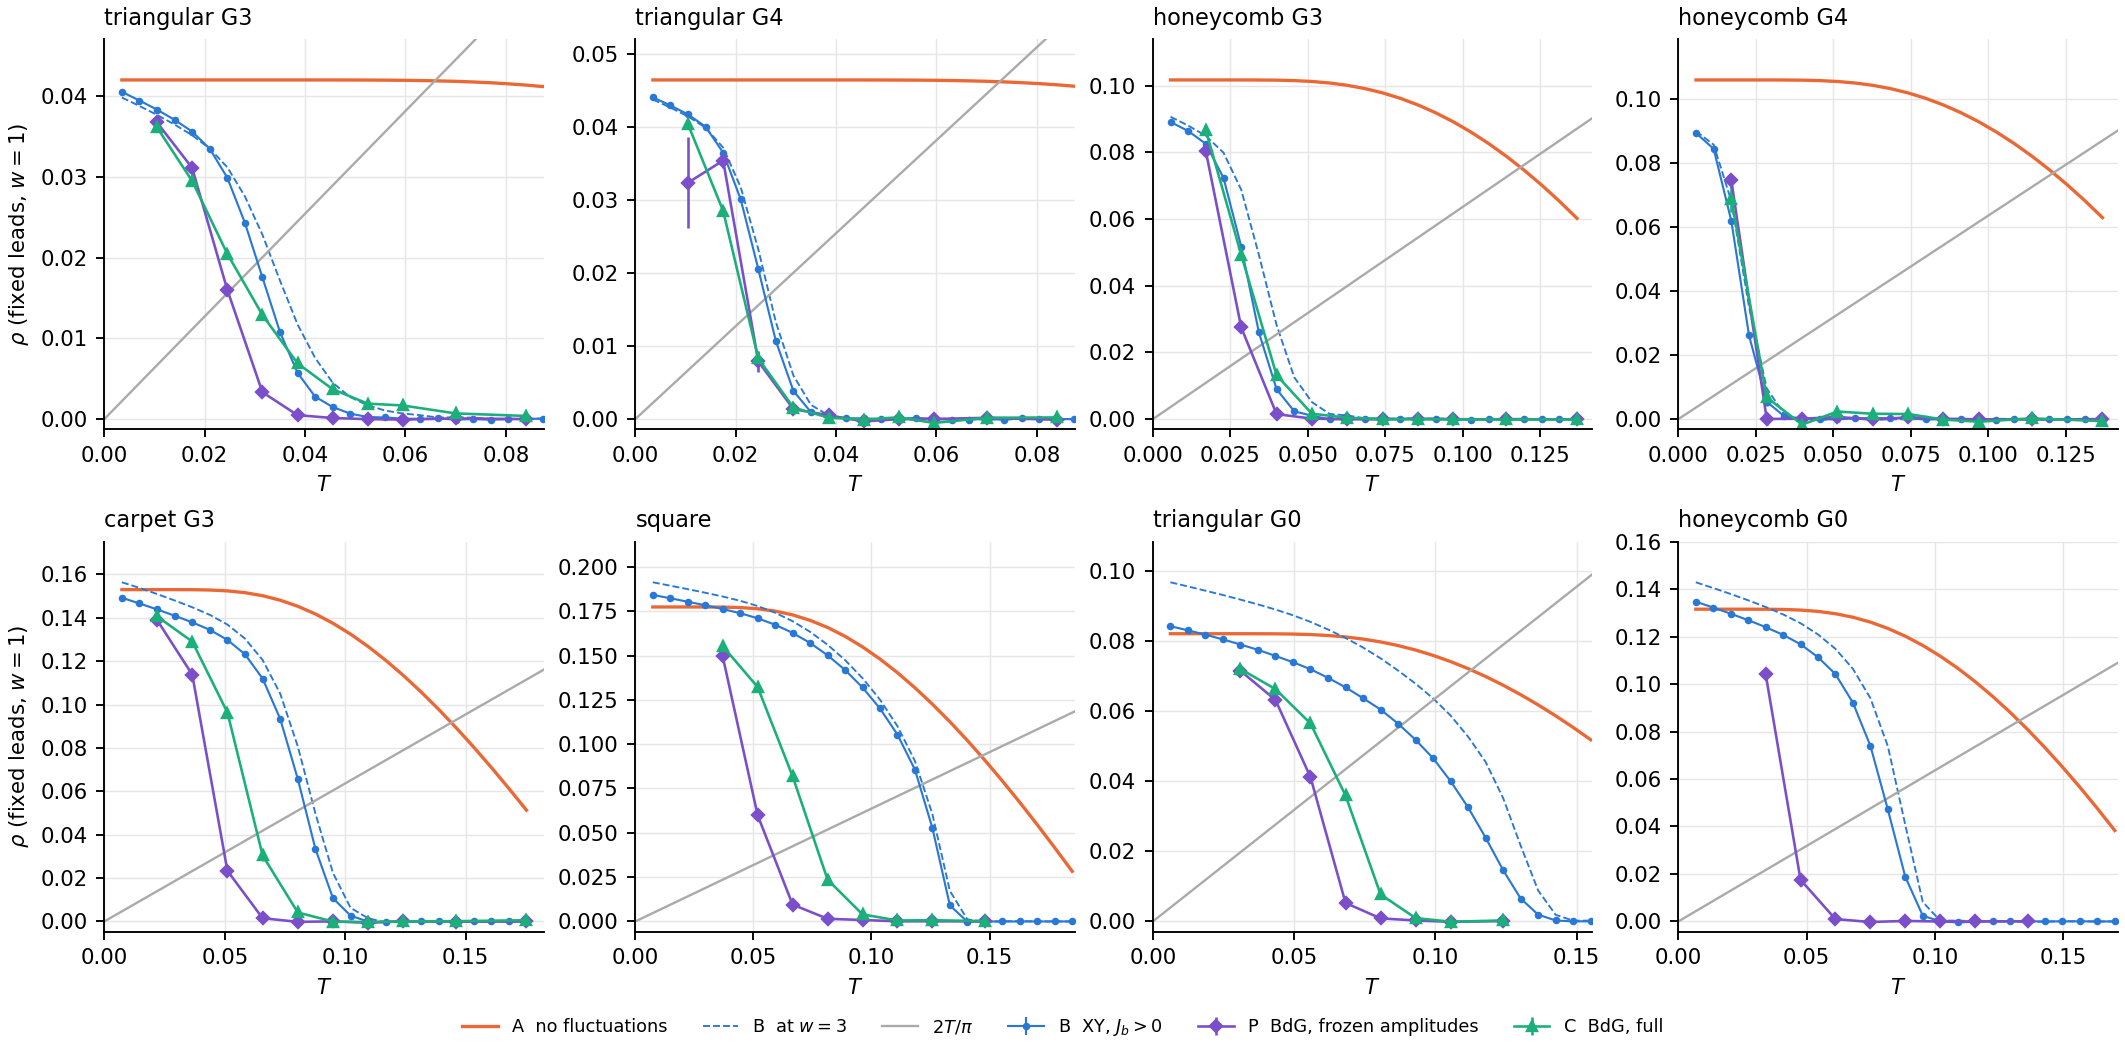
\includegraphics[width=0.98\textwidth]{u2_ladder.png}
\caption{Complete four-rung stiffness comparison $\rho(T)$ at strong coupling $U=2$ ($w=1$, fixed electron filling) across the fractal and parent lattices: Rung~A (orange), Rung~B (blue solid for $w=1$, dashed for $w=3$), Rung~P (purple diamonds), and Rung~C (green triangles), intersected by the BKT universal line $2T/\pi$ (grey dashed). On finitely ramified gaskets (top row), Rungs~B, P, and C agree within $\sim 15\%$, whereas on the infinitely ramified carpet and filled 2D parents (bottom row), the nearest-neighbor XY approximation significantly overestimates the fermionic crossover.}
\label{fig:u2_ladder}
\end{figure*}

Three fundamental physical lessons emerge from Fig.~\ref{fig:u2_ladder} and Table~\ref{tab:u2}. First, on the finitely ramified triangular and honeycomb gaskets ($G=3$ and $G=4$), the three fluctuating rungs—B, P, and C—agree with one another to within $10\%\text{--}15\%$ ($T_P/T_B \in [0.81, 1.02]$ and $T_C/T_B \in [0.86, 1.04]$). Because fractal localization compresses the Cooper pairs to the single-bond scale and concentrates the phase kernel onto nearest neighbors, the local XY model with temperature-dependent BdG couplings $J_b(T)$ provides a quantitatively accurate effective theory of thermal phase fluctuations on finitely ramified gaskets. At the same time, increasing the coupling from $U=1$ to $U=2$ erases the mean-field pairing advantage of the gaskets: once the bare pairing interaction $U$ becomes comparable to the bandwidth of the spectral sub-clusters, $\Tmf$ converges to $0.18\text{--}0.23$ across all gaskets and filled parents alike (and is even slightly lower on the honeycomb gasket than on honeycomb $G_0$). Meanwhile, the geometric neck bottleneck remains in full force: the true fermionic coherence temperature $T_C$ on the $G=4$ triangular gasket is roughly one-third that of its filled triangular parent and just one-tenth of $\Tmf$ ($T_C/\Tmf \approx 0.10$ on triangular $G=4$ and $0.14$ on honeycomb $G=4$, compared with $0.30\text{--}0.38$ on the carpet and filled lattices). At strong coupling, finitely ramified gaskets are therefore no better than regular crystals in pair formation and substantially worse in phase coherence.

Second, on the infinitely ramified Sierpi\'nski carpet and on all three filled two-dimensional parent lattices, the nearest-neighbor XY mapping (Rung~B) systematically \emph{overestimates} the coherence temperature compared with the exact fermionic functional: Rungs~P and~C cross $2T/\pi$ at only $0.49\text{--}0.76$ of $T_B$ (Fig.~\ref{fig:u2_ladder}, bottom panels). Crucially, at $U=2$ this discrepancy cannot be blamed on contact resistance or on a mismatch of the linear-response stiffness scale, since $\rho_K/\rho_\chi \approx 0.92\text{--}0.97$ and $R = \rho_K/\rho_{\mathrm{harm}} \approx 0.95\text{--}1.01$ at $w=1$ (Table~\ref{tab:uscan}). Indeed, at the lowest temperatures $\rho_P(T)$ and $\rho_C(T)$ start from the same zero-temperature baseline as $\rho_B(T)$, but soften much more rapidly as $T$ increases. The failure of Rung~B on two-dimensional and infinitely ramified networks therefore originates beyond quadratic linear response~\cite{BTC04,EM10}: when a phase twist across a bond becomes large or a vortex core forms, the exact fermionic free energy $F[a_0 e^{i\theta}]$ flattens much sooner than the rigid nearest-neighbor cosine $-\sum_b J_b \cos(\theta_i-\theta_j)$ extruded from infinitesimal twists, and the remaining nonlocality of the phase kernel ($\xi_{\mathrm{pair}} \approx 2$) lowers the cost of short-scale phase windings and vortex cores (as we demonstrate directly in Section~\ref{sec:vortex_bdg_barriers}).

Third, comparing Rung~C against Rung~P reveals the nontrivial role of thermal amplitude fluctuations. While freeing the amplitudes changes the crossover temperature on the gaskets by less than $16\%$, on the carpet and filled lattices it consistently \emph{raises} the stiffness and increases the crossover temperature by $13\%\text{--}29\%$ ($T_C/T_P = 1.28$ on the carpet, $1.29$ on the square, and $1.13$ on triangular $G_0$). The physical origin of this stiffening can be traced to the gap-to-noise ratio $a_0 / \sqrt{UT_\times}$ in Table~\ref{tab:uscan}: on the triangular gasket, the crossover $T_\times$ occurs at a low reduced temperature $T_\times/\Tmf \approx 0.31$ where the mean-field gap is large compared with thermal amplitude noise ($a_0/\sqrt{UT_\times} \approx 1.01$). On the carpet and square lattice, however, the crossover occurs much higher up the dome ($T_\times/\Tmf \approx 0.70$), where $a_0/\sqrt{UT_\times} \approx 0.52\text{--}0.56$ is moderate. In this regime, thermal fluctuations of the pairing modulus skew the mean-square gap $\langle |\Delta_i|^2 \rangle$ upward relative to its saddle-point value $a_{0,i}^2$, reinforcing the effective local phase stiffness against phase disordering.

\begin{figure*}[htbp]
\centering
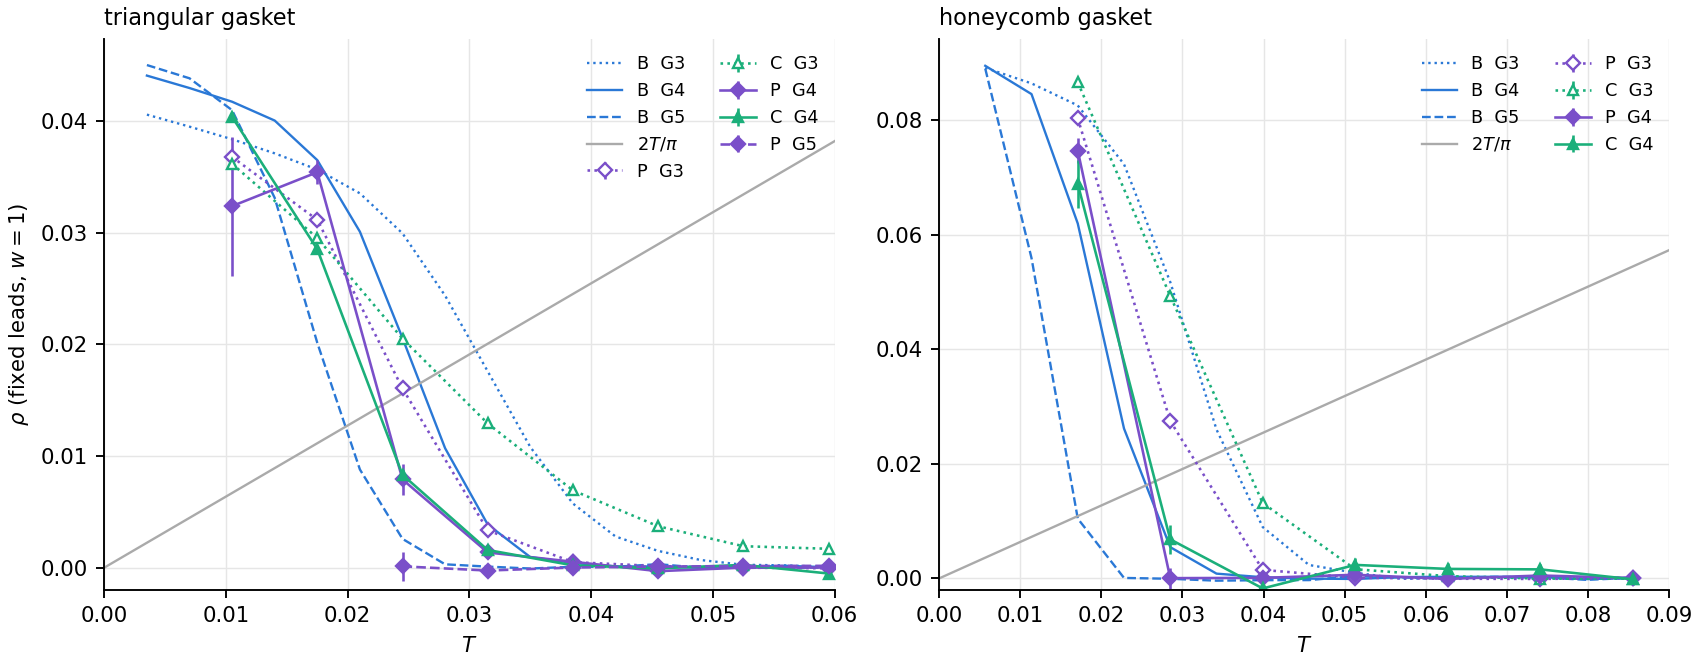
\includegraphics[width=0.92\textwidth]{u2_sizes.png}
\caption{Generation scaling of the two-terminal superfluid stiffness $\rho(T)$ at $U=2$ ($w=1$) on the triangular gasket (left) and honeycomb gasket (right) across generations $G=3$ (open markers, dotted lines), $G=4$ (filled markers, solid lines), and $G=5$ (dashed lines) for Rungs~B (blue), P (purple), and C (green). The crossover temperature decreases monotonically with generation at the rate predicted by the classical uniform-$J$ XY scaling exponent.}
\label{fig:u2_sizes}
\end{figure*}

\begin{figure*}[htbp]
\centering
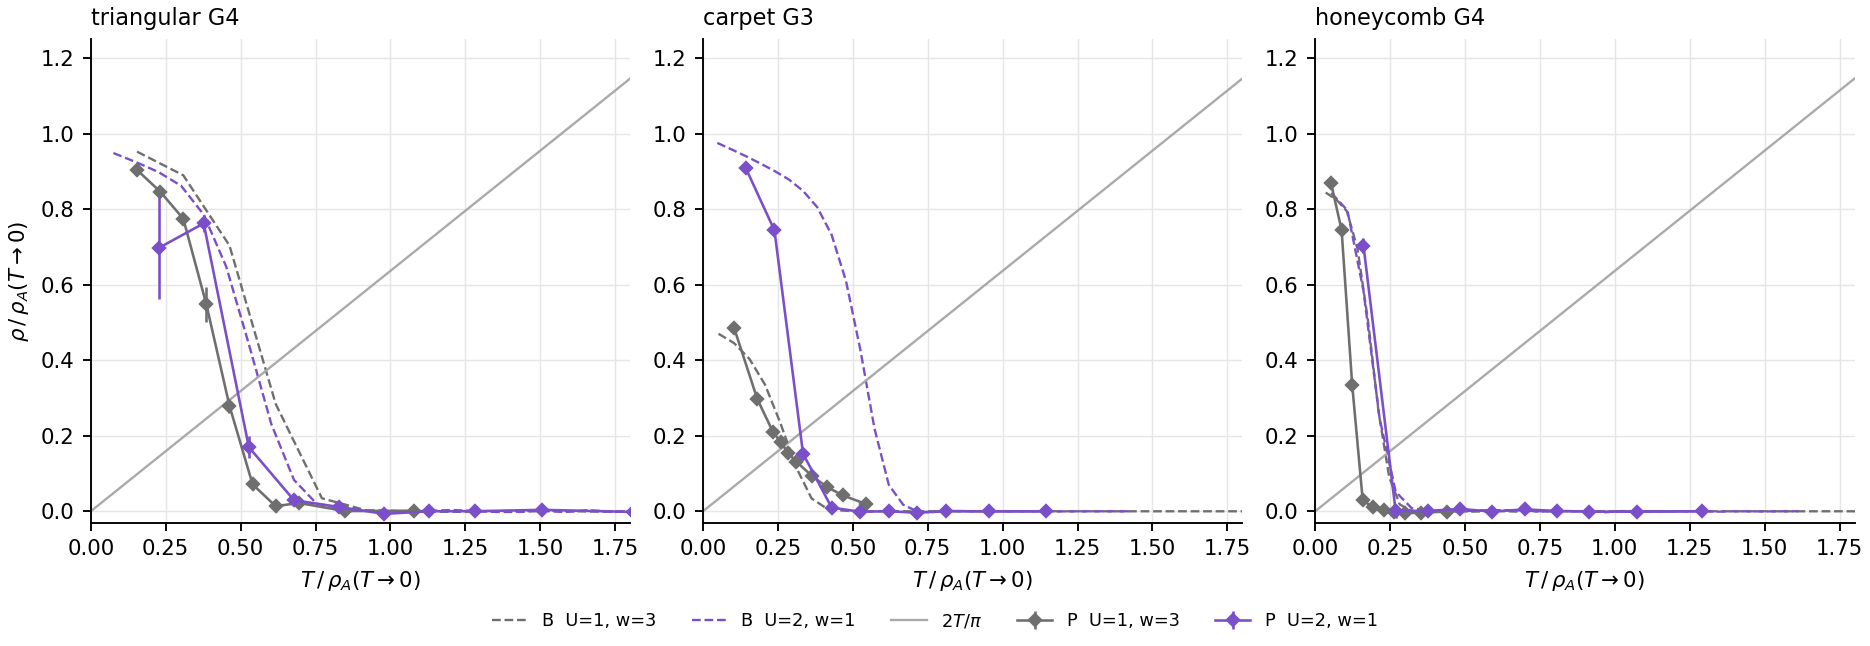
\includegraphics[width=0.92\textwidth]{u2_u1_vs_u2.png}
\caption{Universal scaling comparison between intermediate coupling ($U=1$, $w=3$, grey) and strong coupling ($U=2$, $w=1$, purple) for Rung~B and Rung~P, with both temperature and stiffness normalized by the zero-temperature no-fluctuation scale $\rho_A(T\to 0)$. On both gaskets (left and right), the dimensionless stiffness curves collapse across couplings, whereas the carpet (center) recovers its full low-temperature stiffness at $U=2$ once negative projected couplings and contact losses are eliminated.}
\label{fig:u2_u1_vs_u2}
\end{figure*}

Tracking the gasket crossover across three successive generations $G=3 \to 4 \to 5$ at $U=2$ (Fig.~\ref{fig:u2_sizes} and Table~\ref{tab:u2}) connects our microscopic fermionic simulations directly to the thermodynamic scaling theorems of finitely ramified fractals~\cite{GMA80,GAM83,Vallat1991,MB10}. On the triangular gasket, $T_B$ drops by a factor of $0.85$ from $G=3$ to $G=4$ and by $0.76$ from $G=4$ to $G=5$, while the full fermionic crossing $T_C$ falls by $0.82$ from $G=3$ to $G=4$ (and Rung~P at $G=5$ vanishes at all $T \ge 0.0245$, consistent with $T_B = 0.0198$). On the honeycomb gasket, $T_B$ falls by $0.72$ and $0.67$ across the same steps, matched by $T_C$ falling by $0.72$ from $G=3$ to $G=4$. As established in our uniform-$J$ classical XY scaling analysis, a power-law decay of the finite-size crossover $T^*(G) \propto L^{-x}$ with linear system size $L = 2^G$ and exponents $x \approx 0.50$ (triangular) and $x \approx 0.56$ (honeycomb) predicts per-generation reduction factors of $2^{-0.50} \approx 0.71$ and $2^{-0.56} \approx 0.68$. The self-consistent fermionic superconductor on a gasket thus obeys the exact same asymptotic generation decay as the uniform classical XY model, demonstrating that the finite-size coherence crossover vanishes as $G \to \infty$. Furthermore, when both $\rho(T)$ and $T$ are rescaled by the zero-temperature mean-field stiffness $\rho_A(T\to 0)$ (Fig.~\ref{fig:u2_u1_vs_u2}), the Rung~B and Rung~P curves of the gaskets at $U=1$ and $U=2$ collapse onto a universal master curve, whereas the carpet recovers from its anomalous $U=1$ suppression ($\rho_P(T\to 0)/\rho_A \approx 0.49$) to normal low-temperature rigidity ($\rho_P(T\to 0)/\rho_A \approx 0.90$) at $U=2$.

\begin{figure*}[htbp]
\centering
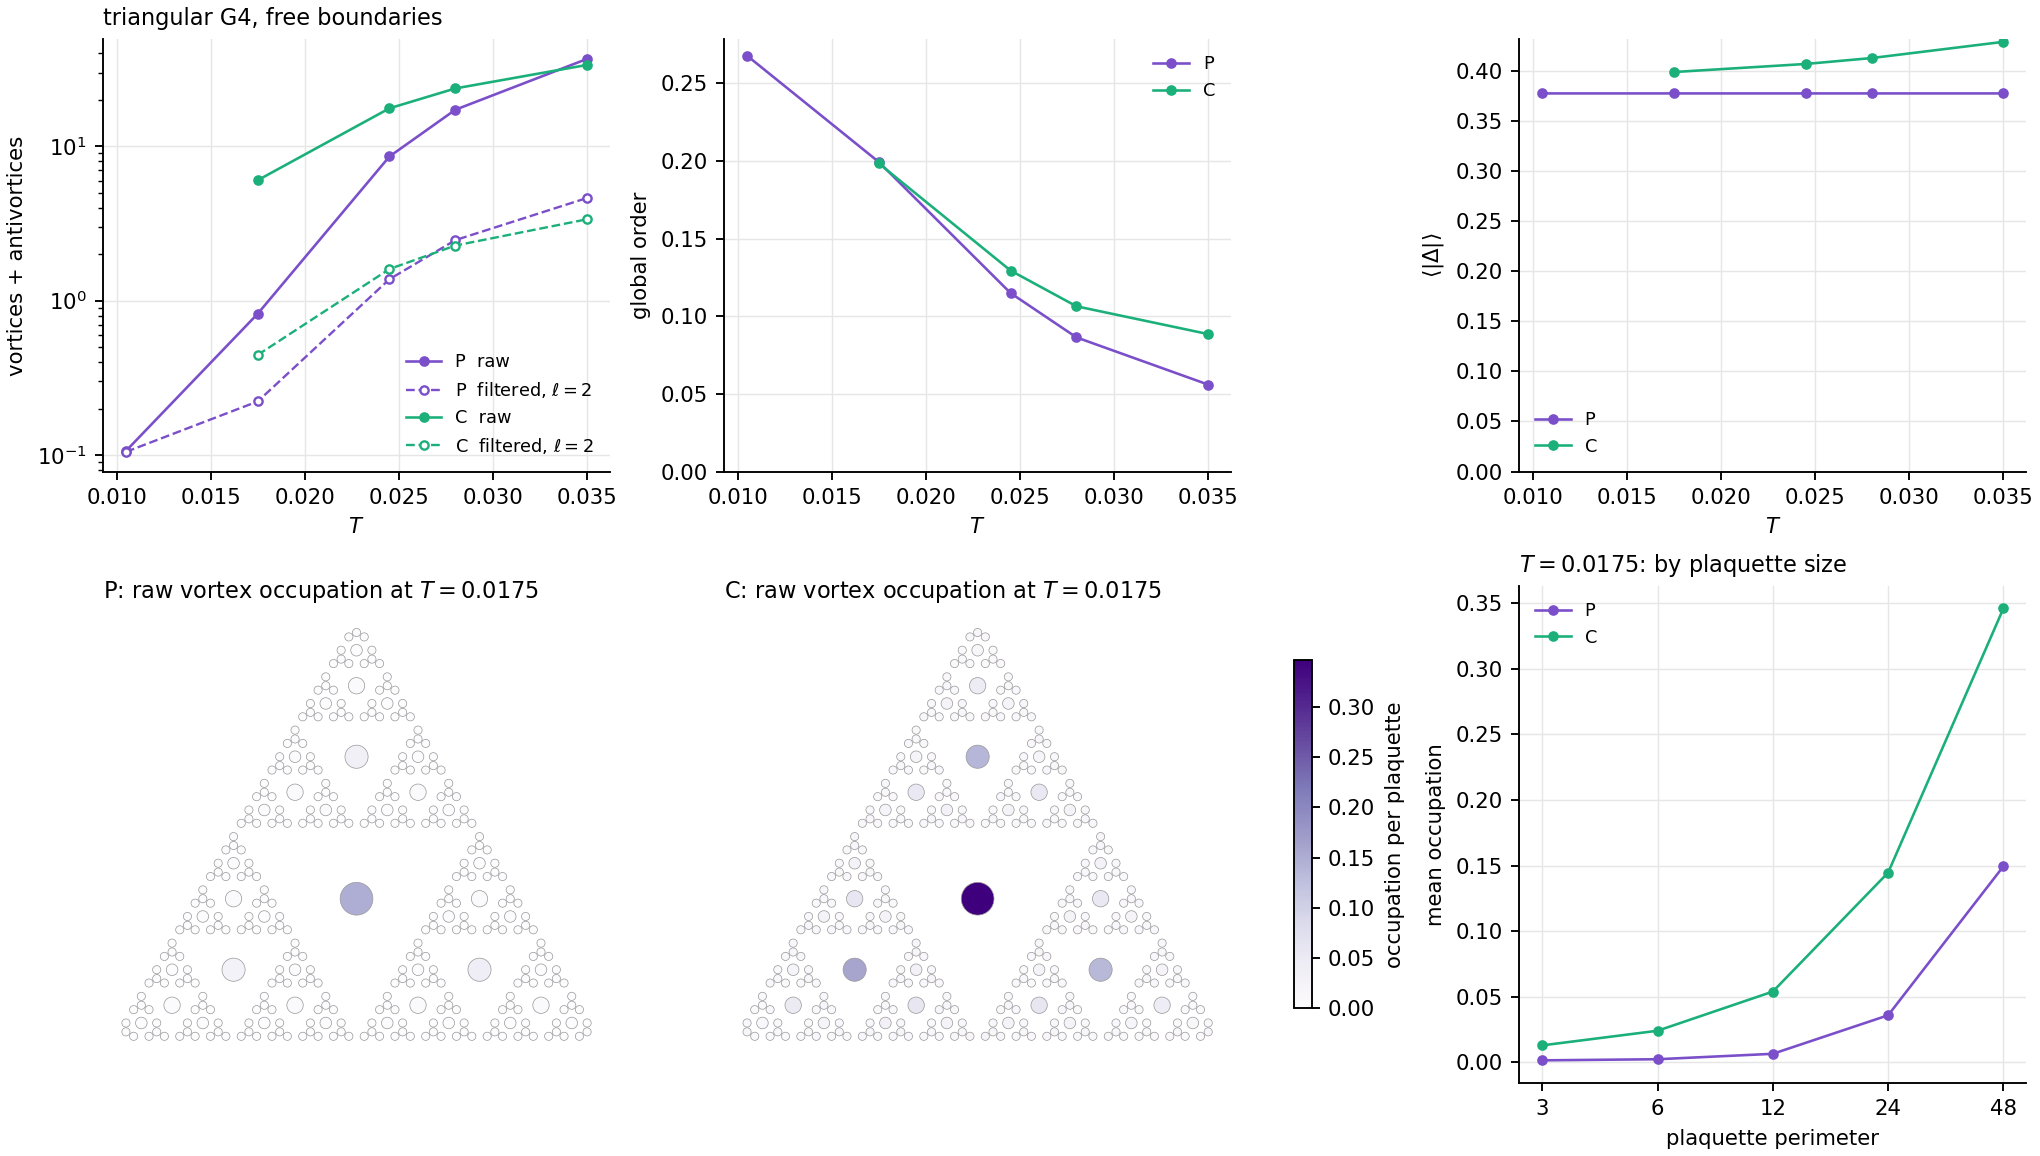
\includegraphics[width=0.95\textwidth]{u2_free_triangular_G4.png}
\caption{Free-boundary static-path BdG Monte Carlo diagnostics on the $G=4$ triangular gasket at $U=2$, comparing Rung~P (frozen amplitudes, purple) and Rung~C (full amplitude and phase fluctuations, green). Top row: total number of vortices plus antivortices $N_v$ counted raw ($\ell=0$) and after applying a graph heat-kernel filter $W_\ell = e^{-\ell^2\mathcal{L}/4}$ of smoothing length $\ell=2,4$ to $\Delta_i$, global condensate fraction $|N^{-1}\sum_i \Delta_i|$, and unaveraged modulus $\langle |\Delta_i| \rangle$. Bottom row: spatial map of raw vortex occupation per face at $T=0.0175$ and mean occupation stratified by lacuna perimeter $P$. Filtering out short-scale amplitude noise collapses the physical vortex count and global order of Rungs~P and~C onto one another.}
\label{fig:u2_free_triangular_G4}
\end{figure*}

\begin{figure*}[htbp]
\centering
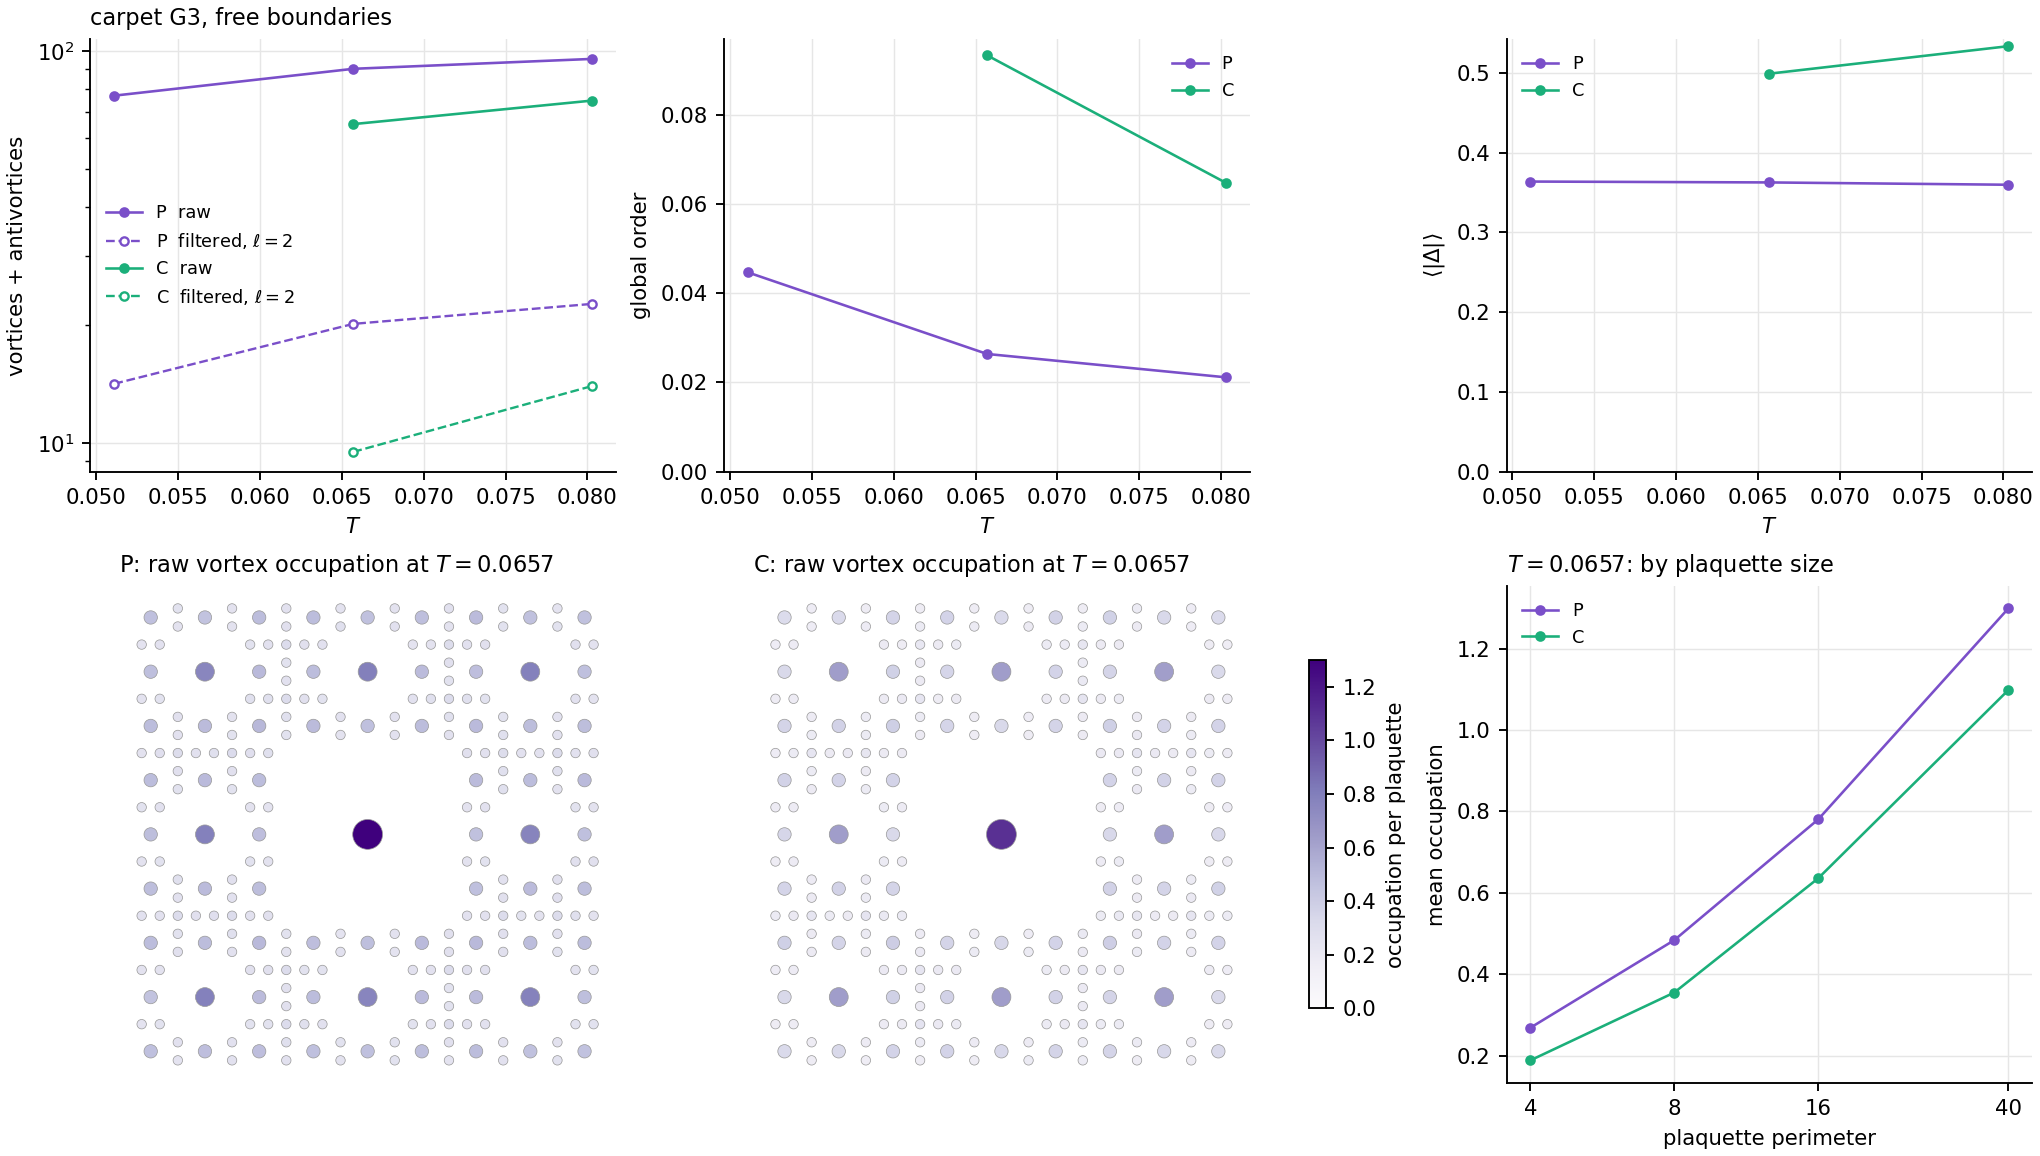
\includegraphics[width=0.95\textwidth]{u2_free_carpet_G3.png}
\caption{Free-boundary static-path BdG Monte Carlo diagnostics on the $G=3$ Sierpi\'nski carpet at $U=2$ for Rung~P and Rung~C. Top row: raw and heat-kernel-filtered vortex counts, global order parameter $|N^{-1}\sum_i \Delta_i|$, and mean modulus $\langle |\Delta_i| \rangle$. Bottom row: spatial map of vortex occupation across internal lacunae and perimeter-stratified occupation, showing strong concentration in the central $P=40$ hole and fewer vortices (alongside stronger global phase order) in Rung~C than in Rung~P, consistent with $T_C > T_P$.}
\label{fig:u2_free_carpet_G3}
\end{figure*}

Finally, running Rungs~P and~C with free boundaries (no pinned leads) allows us to directly image the spatial distribution of topological defects and the global condensate order parameter $|N^{-1}\sum_i \Delta_i|$ without contact bias (Figs.~\ref{fig:u2_free_triangular_G4} and~\ref{fig:u2_free_carpet_G3}). On the $G=4$ triangular gasket at $T=0.0175$ (just below the BKT crossover), vortex occupation is overwhelmingly concentrated in the hierarchy of internal lacunae, rising steeply with hole perimeter $P$ and peaking in the central $P=48$ lacuna. At first glance, raw phase-winding counts ($\ell=0$) in Rung~C appear to show nearly an order of magnitude more vortices at low temperature than in Rung~P. However, applying a graph heat-kernel smoothing filter $W_\ell = \exp(-\ell^2 \mathcal{L}/4)$ of range $\ell = 2$ or $4$ lattice spacings to the complex field $\Delta_i$ before evaluating plaquette windings—which smooths ultraviolet fluctuations over elementary triangles without crossing internal lacunae—eliminates this excess and collapses the filtered vortex density of Rung~C onto that of Rung~P, while the global order parameter $|N^{-1}\sum_i \Delta_i|$ is identical in both rungs. The extra raw windings in Rung~C are therefore not macroscopic topological defects, but short-scale phase jitter on individual elementary triangles where thermal $\sqrt{UT}$ amplitude noise momentarily drives $|\Delta_i|$ close to zero. On the Sierpi\'nski carpet (Fig.~\ref{fig:u2_free_carpet_G3}), vortices similarly accumulate in the large central $P=40$ lacuna, and Rung~C exhibits both a lower vortex count and a larger global condensate fraction than Rung~P at the same temperature, independently confirming the fixed-lead finding that amplitude fluctuations stabilize phase coherence on the carpet ($T_C > T_P$).

%======================================================================
\section{Vortex Hierarchy, Escape Dynamics, and Current Relaxation}
\label{sec:vortices}
%======================================================================

The collapse of the BKT crossover on finitely ramified fractals and the heavy concentration of topological charges inside large internal lacunae raise a natural dynamical question: do the geometric holes of a fractal merely act as low-energy sinks that flood the sample with vortices, or do they serve as deep pinning traps that arrest vortex motion and protect supercurrent flow over experimental timescales? Answering this question requires a rigorous topological definition of vortex charges, static saddle networks, and time-resolved current relaxation on general non-Euclidean graphs.

%----------------------------------------------------------------------
\subsection{Topological charges, lacuna energy hierarchy, and static versus dynamical escape barriers}
\label{sec:vortex_hierarchy}
%----------------------------------------------------------------------

We formulate the vortex analysis on the coupled subgraph $K = \{b : J_b > 0\}$ of positive nearest-neighbor pair-phase couplings, governed by the XY energy functional
\begin{equation}
E(\bm{\theta}) = -\sum_{b \in K} J_b \cos(\theta_j - \theta_i),
\label{eq:xy_coupled_graph}
\end{equation}
where $J_b(T)$ are either the Stage-1 BdG couplings or uniform reference couplings $J_b = 1$, and energies are measured relative to the uniform ground state $E_0 = -\sum_{b\in K} J_b$ in units of the mean positive coupling $\bar{J} = |K|^{-1}\sum_{b\in K} J_b$. Removing any bond with $J_b \le 0$ merges the two elementary lattice faces on either side of that bond into a single cycle of $K$ (and any face that merges with the exterior boundary loses its topological enclosure). The chordless planar cycles $f \in F$ of $K$ thus partition into three distinct classes: elementary \emph{small} plaquettes of the underlying lattice, internal \emph{lacunae} enclosing geometric holes of perimeter $P_f$ bonds, and \emph{merged} faces formed where weak or negative BdG couplings open internal walls on the carpet. On every graph studied, we verify Euler's cycle-basis identity $|F| = |K| - V + 1$, guaranteeing that the face charges form a complete topological basis.

To track vortex motion without ambiguity, we assign to each directed bond $b = (i \to j) \in K$ an integer branch winding number $n_b = \operatorname{round}[(\theta_j - \theta_i)/2\pi]$. Because the raw phase differences $\theta_j - \theta_i$ sum identically to zero around any closed loop, the topological vorticity (charge) $q_f \in \mathbb{Z}$ of face $f$ resides entirely in the branch integers:
\begin{equation}
q_f = \frac{1}{2\pi}\sum_{b \in \partial f} C_{fb}\bigl[\theta_j - \theta_i - 2\pi n_b\bigr] = -\sum_{b \in K} C_{fb}\,n_b,
\label{eq:topological_charge}
\end{equation}
where $C_{fb} \in \{0, \pm 1\}$ is the oriented face--bond curl incidence matrix. Equation~\eqref{eq:topological_charge} makes the microscopic kinematics of vorticity explicit: a face charge $q_f$ can change if and only if a single bond $b$ undergoes a discrete phase \emph{slip} ($\Delta n_b = \pm 1$, when $|\theta_j - \theta_i|$ crosses $\pi$), which transfers exactly one unit of topological charge across bond $b$ from the face on one side to the adjacent face on the other (or to the exterior boundary if $b$ lies on the outer perimeter).

Using free boundary conditions so that pinned contacts do not distort the defect energetics, we map out the complete static energy landscape of single vortices across all faces of the fractal flakes. Initializing from the analytical harmonic vortex field on face $f$—whose quadratic continuum energy is $E_h(f) = 2\pi^2 [(C D^{-1} C^T)^{-1}]_{ff}$ with $D = \operatorname{diag}(J_b)$~\cite{JKKN77}—we relax $E(\bm{\theta})$ to a local minimum. Face $f$ is classified as a stable vortex \emph{basin} if the relaxed state retains topological charge $q_{f'} = \delta_{ff'}$ and its site-phase Hessian $H = B^T \operatorname{diag}(J_b\cos\Delta\theta_b) B$ is strictly positive definite (apart from the global $\mathrm{U}(1)$ zero mode); the resulting excess energy $E_1(f) = E_{\min}(f) - E_0$ defines the single-vortex creation cost inside lacuna $f$. To construct the transition network connecting all stable basins $h$ (including the vortex-free exterior vacuum $h=0$), we initiate bond-crossing trajectories across every perimeter bond of each basin, relax the minimum-energy paths using the simplified string method~\cite{ERV} preconditioned in the metric of the coupling Laplacian $L = B^T D B$ (where $H \preceq L$ guarantees unconditional stability for step sizes below $2$), and converge the highest image to machine precision via Newton iteration. A stationary point is accepted as a genuine transition \emph{saddle} only if its Hessian possesses exactly one negative eigenvalue and steepest-descent relaxation along the two opposite directions of the unstable eigenvector terminates in distinct basins $h \neq h'$. From this verified graph of minima and index-$1$ saddles, minimax graph search yields the directed transition barrier $B(h \to h')$ (the lowest possible highest saddle energy along any path from $h$ to $h'$, minus $E_1(h)$), the basin \emph{escape barrier}
\begin{equation}
B_{\mathrm{esc}}(h) = \min_{h' \neq h} B(h \to h'),
\label{eq:escape_barrier}
\end{equation}
the boundary \emph{entry barrier} $E_{\mathrm{in}}(h) \ge E_1(h) + B_{\mathrm{esc}}(h)$ from the exterior vacuum, the vortex--antivortex \emph{pair-creation saddle} $E_{\mathrm{pair}}(h,h')$ between neighboring basins, and—under rigid contact boundary conditions where crossing the sample shifts the inter-lead phase by $2\pi$—the macroscopic phase-slip \emph{crossing barrier} $E_{\mathrm{cross}}$. Checking this static machinery on uniform regular lattices reproduces the classic Peierls pinning barriers of the square lattice ($0.1996\,J$ versus the literature value $0.20\,J$~\cite{HW}) and triangular lattice ($0.0440\,J$ versus $0.043\,J$~\cite{Lobb,YS}), while identifying a bulk Peierls barrier of $0.580\,J$ on the honeycomb lattice.

\begin{table*}[htbp]
\caption{Hierarchical vortex energetics and Arrhenius escape dynamics in the XY model stratified by lacuna perimeter $P$, comparing Stage-1 BdG couplings $J_b(T)$ at $U=1$ ($T=0.008$ on triangular $G=4$, $T=0.014$ on honeycomb $G=4$, and $T=0.010$ on carpet $G=3$) against uniform couplings $J_b = 1$. Listed for each perimeter class are the number of faces $n$ of that perimeter, the static single-vortex energy $E_1$, the free-boundary Monte Carlo occupation slope against $\bar{J}/T$, the static escape barrier $B_{\mathrm{esc}}$, the committed-event Monte Carlo Arrhenius escape slope $\varepsilon$, and the static entry barrier from the exterior $E_{\mathrm{in}}$ (all energies are medians in units of the mean positive coupling $\bar{J}$).}
\label{tab:vortex_sizes}
\begin{ruledtabular}
\begin{tabular}{lccccccc}
System & $P$ & $n$ & $E_1$ & Occupation slope & $B_{\mathrm{esc}}$ & Escape slope $\varepsilon$ & $E_{\mathrm{in}}$ \\
\hline
Triangular $G=4$, BdG $J_b$ & 6 & 27 & 7.51 & 6.20 & 0.45 & 1.34 & 7.88 \\
 & 12 & 9 & 4.67 & 5.17 & 1.75 & 1.62 & 6.42 \\
 & 24 & 3 & 2.76 & 3.02 & 3.06 & 3.04 & 5.82 \\
 & 48 & 1 & 1.53 & 1.70 & 3.85 & 4.05 & 5.38 \\
\hline
Triangular $G=4$, uniform $J$ & 6 & 27 & 6.30 & 6.14 & 0.23 & 0.28 & 6.49 \\
 & 12 & 9 & 3.97 & 4.11 & 1.29 & 1.27 & 5.26 \\
 & 24 & 3 & 2.26 & 2.34 & 2.38 & 2.50 & 4.64 \\
 & 48 & 1 & 1.28 & 1.65 & 3.06 & 3.35 & 4.34 \\
\hline
Honeycomb $G=4$, BdG $J_b$ & 12 & 27 & 2.17 & 1.93 & 0.75 & 0.06 & 3.04 \\
 & 24 & 9 & 1.50 & 1.50 & 1.57 & 1.41 & 3.11 \\
 & 48 & 3 & 0.89 & 1.14 & 2.06 & 2.05 & 3.04 \\
 & 96 & 1 & 0.51 & -- & 2.34 & 2.32 & 3.11 \\
\hline
Honeycomb $G=4$, uniform $J$ & 12 & 27 & 2.20 & 2.13 & 0.55 & 0.63 & 2.73 \\
 & 24 & 9 & 1.34 & 1.37 & 1.05 & 1.14 & 2.39 \\
 & 48 & 3 & 0.76 & 0.78 & 1.45 & 1.54 & 2.21 \\
 & 96 & 1 & 0.43 & -- & 1.69 & 1.78 & 2.11 \\
\hline
Carpet $G=3$, BdG $J_b$ & 6 & 8 & 1.66 & -- & 0.00 & -- & 1.66 \\
 & 8 & 8 & 1.89 & -- & 0.03 & -- & 1.97 \\
 & 12 & 4 & 1.43 & 0.72 & 0.05 & 0.55 & 1.73 \\
 & 20 & 4 & 1.30 & 0.72 & 0.18 & 0.56 & 1.73 \\
 & 28 & 4 & 0.58 & 0.54 & 0.03 & $-0.06$ & 0.61 \\
 & 40 & 1 & 0.78 & -- & 0.70 & -- & 1.73 \\
\hline
Carpet $G=3$, uniform $J$ & 8 & 64 & 3.95 & 3.38 & 0.17 & $-0.12$ & 4.83 \\
 & 16 & 8 & 2.83 & 3.22 & 1.40 & 1.47 & 4.24 \\
 & 40 & 1 & 1.84 & 1.98 & 2.68 & 2.41 & 4.83 \\
\end{tabular}
\end{ruledtabular}
\end{table*}

\begin{figure*}[htbp]
\centering
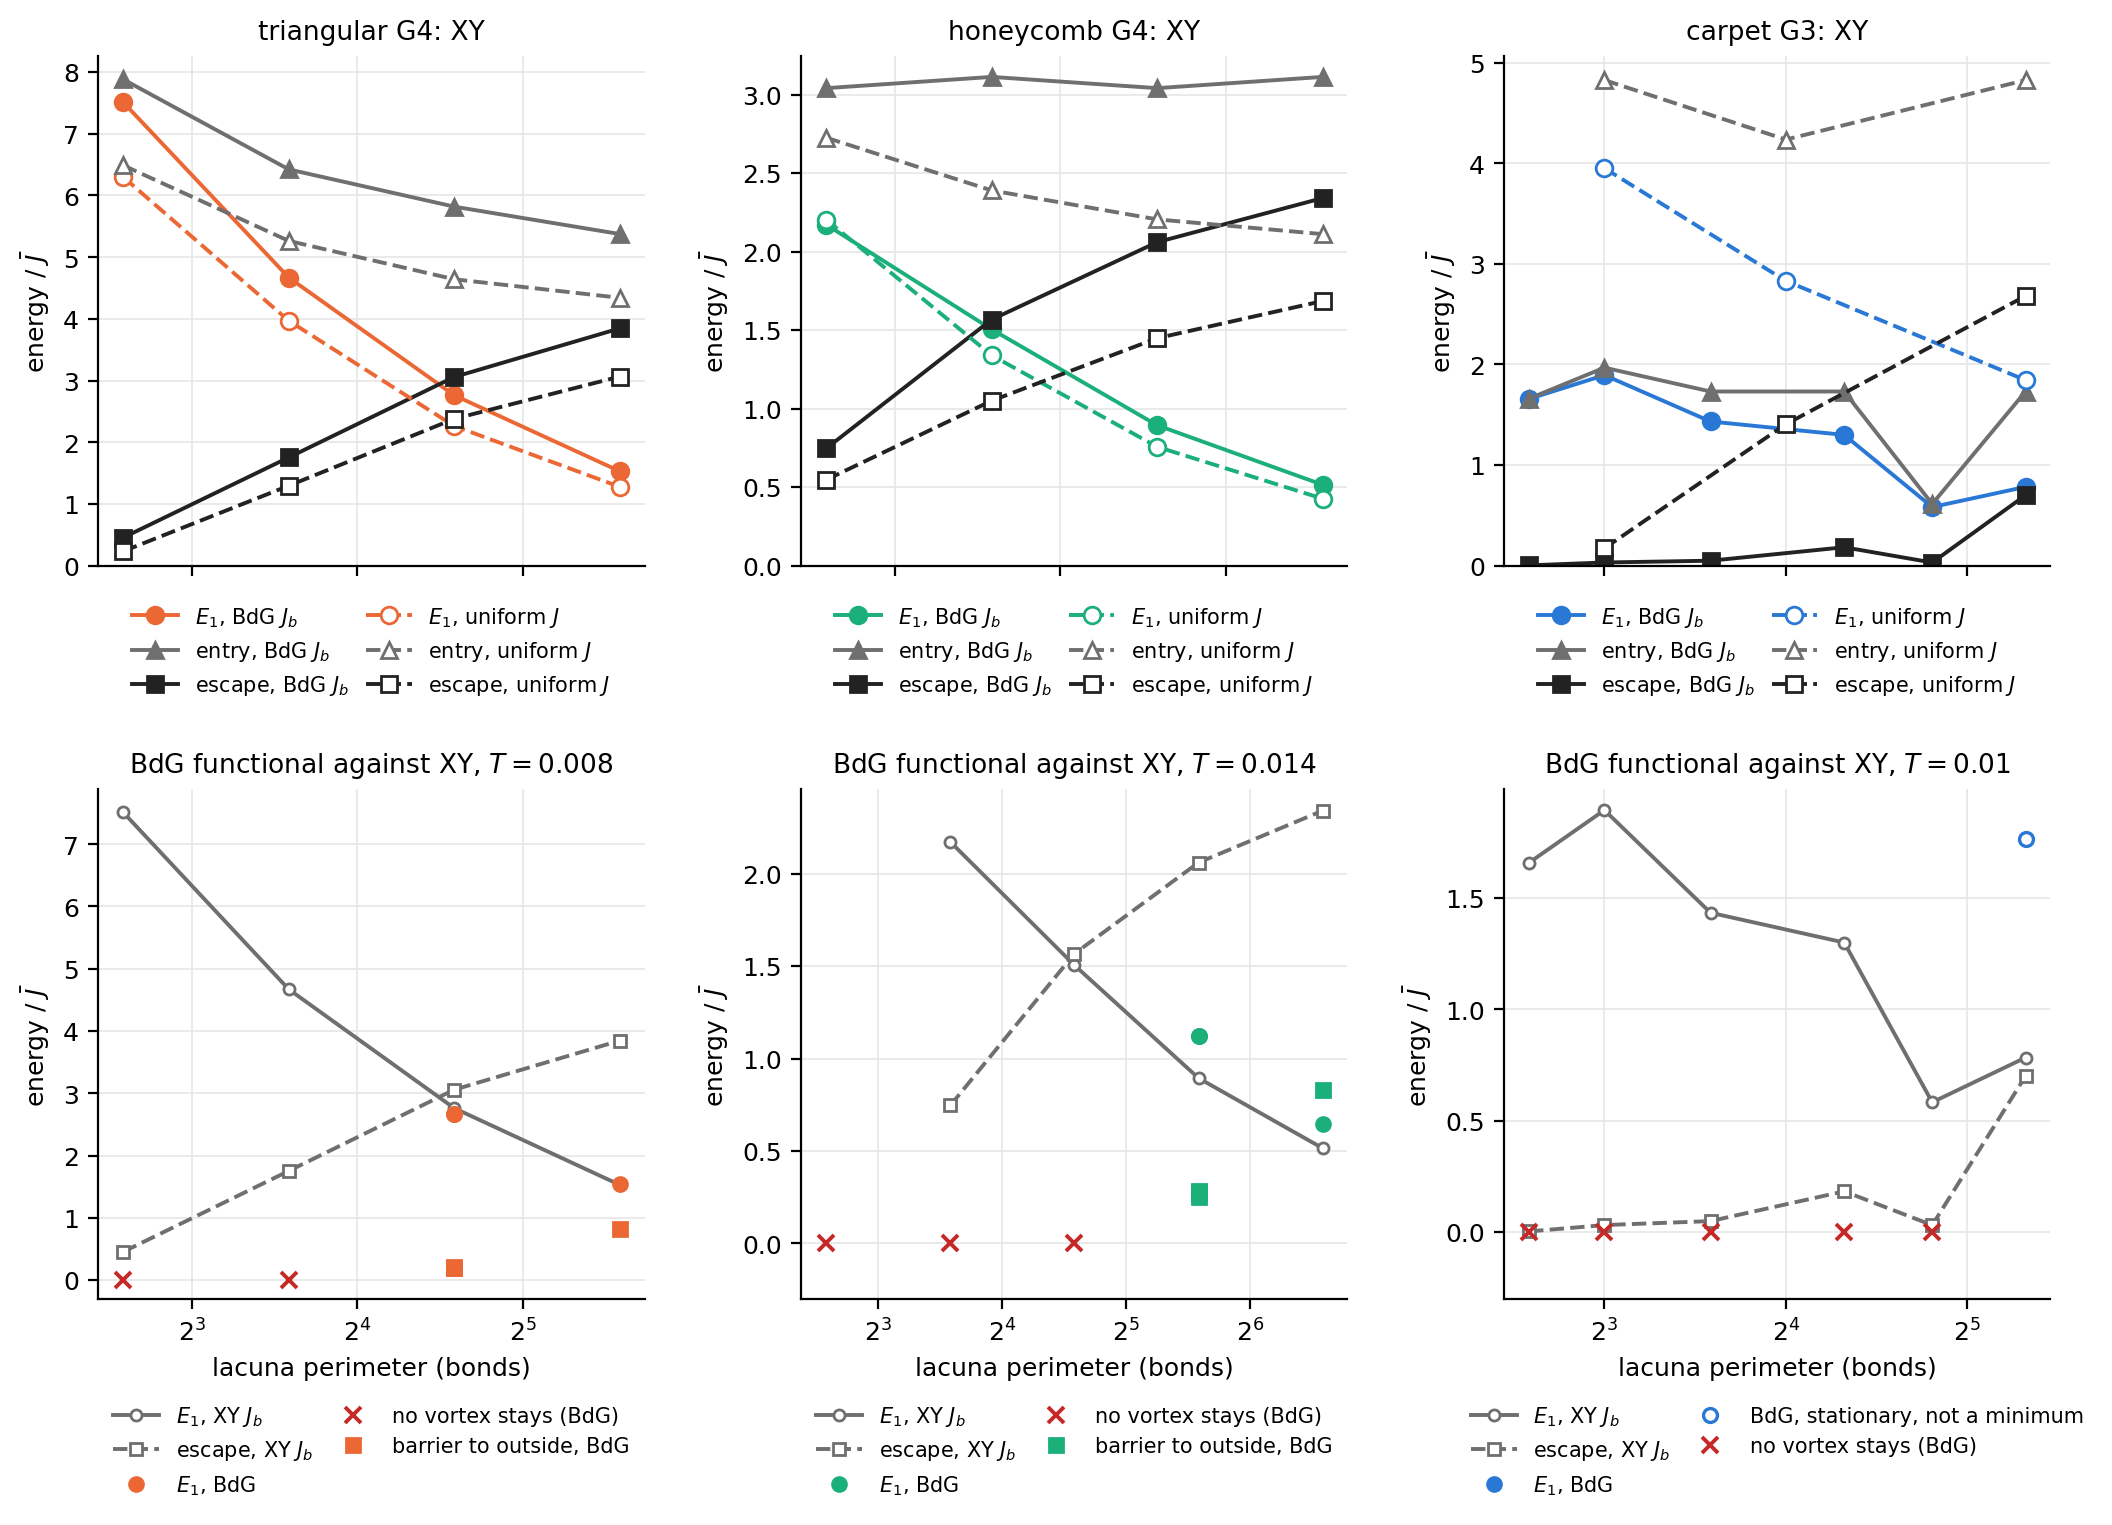
\includegraphics[width=0.95\textwidth]{vortex_energies.png}
\caption{Hierarchical vortex energy landscape across lacuna perimeters $P$ on the triangular gasket $G=4$, honeycomb gasket $G=4$, and Sierpi\'nski carpet $G=3$. Top row: static XY single-vortex energy $E_1$, escape barrier $B_{\mathrm{esc}}$, and exterior entry barrier $E_{\mathrm{in}}$ (in units of $\bar{J}$) for uniform couplings and Stage-1 BdG couplings $J_b$, demonstrating the inverse scaling of $E_1 \propto P^{-0.8}$ and the monotonic growth of $B_{\mathrm{esc}}$ with perimeter. Bottom row: comparison of vortex energies and exterior escape barriers $B_{\mathrm{out}}$ in the full BdG functional $F[\Delta]$ against the local XY model with $J_b$ (the open circle on the carpet at $T=0.01$ marks a symmetric saddle point rather than a stable minimum).}
\label{fig:vortex_energies}
\end{figure*}

The static energy hierarchy of the fractal lacunae is presented in Table~\ref{tab:vortex_sizes} and the top panels of Fig.~\ref{fig:vortex_energies}. On both gaskets—with either uniform couplings or Stage-1 BdG couplings $J_b(T)$—all $40$ internal lacunae support locally stable single-vortex states, and their energetics organize into a striking inverted funnel controlled by the lacuna perimeter $P$. Because a larger hole removes the high-gradient core region of the phase field while distributing the $2\pi$ winding over $P$ perimeter bonds, the single-vortex creation energy $E_1(P)$ drops rapidly with perimeter, following a power law $E_1(P) \propto P^{-\alpha}$ with $\alpha \approx 0.77\text{--}0.78$ (falling by a factor of $1.6\text{--}1.8$ with each doubling of $P$). Simultaneously, the escape barrier $B_{\mathrm{esc}}(P)$ required to push the vortex out of the lacuna across the surrounding narrow necks rises monotonically with $P$, growing nearly tenfold from the smallest to the largest central hole on the triangular gasket. Small lacunae are therefore high-energy, shallow metastable states, whereas the large central lacunae act as deep, low-energy topological traps. Furthermore, comparing $G=3$, $4$, and $5$ shows that $E_1(P)$ and $B_{\mathrm{esc}}(P)$ depend almost exclusively on the local perimeter $P$ rather than on the overall gasket generation $G$ (shifting by less than $7\%\text{--}10\%$ across generations). Consequently, the macroscopic phase-slip barrier $E_{\mathrm{cross}}$ for a vortex to traverse the entire flake between the contacts saturates to a small, generation-independent constant on finitely ramified gaskets ($4.60, 4.34, 4.20\,J$ for triangular $G=3,4,5$ and $2.19, 2.11, 2.07\,J$ for honeycomb $G=3,4,5$ at uniform $J$, or $5.68\,\bar{J}$ and $3.07\,\bar{J}$ with BdG couplings, compared with $17\text{--}18\,\bar{J}$ on the filled triangular and square parent flakes). On the Sierpi\'nski carpet with $U=1$ BdG couplings, by contrast, the removal of the $15\%$ frustrated negative bonds breaches the walls of most cutouts, leaving only $21$ of $57$ lacunae (plus $8$ merged faces) able to hold a vortex and collapsing the median escape barrier to just $0.03\,\bar{J}$.

\begin{figure*}[htbp]
\centering
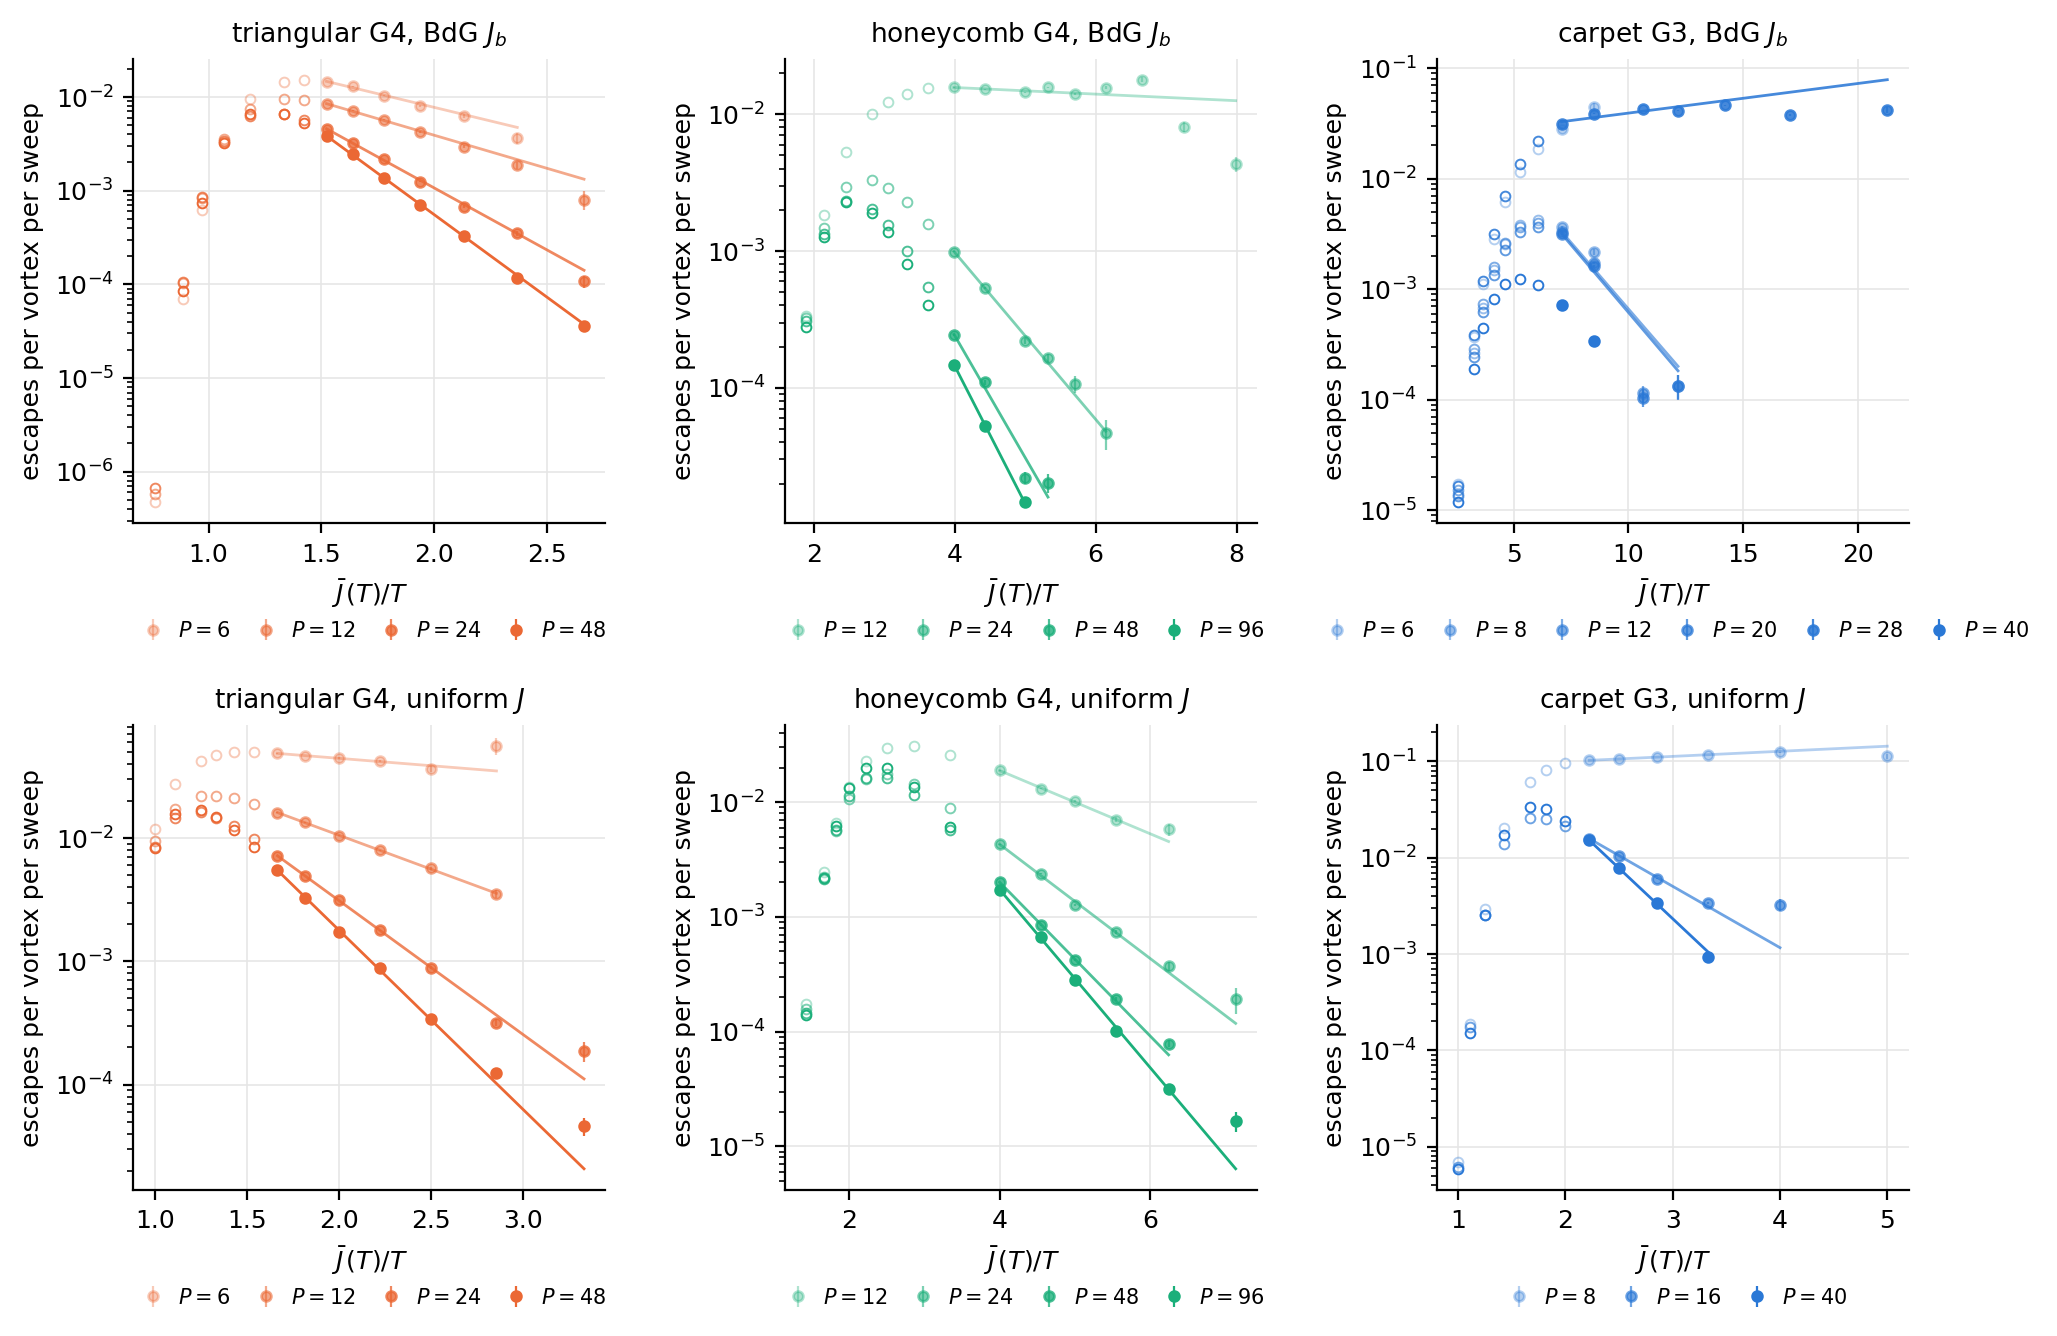
\includegraphics[width=0.95\textwidth]{vortex_escape_rates.png}
\caption{Arrhenius plot of the committed-event Monte Carlo vortex escape rate $r$ (per occupied sweep) versus inverse reduced temperature $\bar{J}(T)/T$ stratified by lacuna perimeter $P$ across the fractal flakes with Stage-1 BdG couplings $J_b(T)$ and uniform couplings. Filled symbols indicate the dilute vortex regime ($\le 1.5$ vortices per flake on average) used for Poisson maximum-likelihood Arrhenius fits (solid lines); open symbols denote higher temperatures where multi-vortex crowding biases event pairing. The fitted dynamical activation slopes reproduce all 14 static saddle barriers $B_{\mathrm{esc}} > 1\,\bar{J}$ to within $\sim 10\%$.}
\label{fig:vortex_escape_rates}
\end{figure*}

To test whether these zero-temperature static saddle barriers govern actual thermal vortex motion at finite temperature, we track individual bond phase slips in real time during free-boundary Metropolis Monte Carlo simulations. Two methodological precautions are essential for extracting unbiased dynamical rates. First, if the Metropolis proposal width $\delta$ were retuned at each temperature to maintain constant acceptance, the physical time represented by one Monte Carlo sweep would vary with $T$ and corrupt Arrhenius slopes. We instead employ a temperature-scaled uniform proposal $\Delta\theta_i \in [-\delta, \delta]$ with variance $\delta^2 = c\,T/J_{\mathrm{ref}}$ ($c=1$, $J_{\mathrm{ref}} = \bar{J}(T_{\min})$). By the Einstein relation, a site seeing a local harmonic restoring stiffness $k \sim z J_b$ experiences a dimensionless step parameter $\beta k \delta^2 = c z J_b / J_{\mathrm{ref}}$ that is independent of temperature, ensuring that one sweep corresponds to a strictly constant physical time interval
\begin{equation}
\Gamma\,\mathrm{d}t = \frac{a_2 c}{6 J_{\mathrm{ref}}} = \frac{c}{6 J_{\mathrm{ref}} f}, \qquad a_2 = \frac{\langle x^2 a(x) \rangle}{\langle x^2 \rangle} = \frac{1}{f},
\label{eq:mc_time_unit}
\end{equation}
across the entire temperature scan, where $a(x)$ is the Metropolis acceptance probability and $f \in [1.9, 3.2]$ is the finite-step mobility factor calibrated below. Second, counting every raw bond slip across a lacuna perimeter overcounts transport by orders of magnitude, because a vortex sitting at a saddle frequently flickers back and forth across a single bond before committing to a basin, and transient virtual dipoles constantly nucleate and recombine across thin walls. We therefore define a \emph{clean time} as any instant when no elementary small plaquette of the lattice carries topological charge, and define a \emph{committed event} as the net change in stable basin charges between consecutive clean times: an opposite pair of charge changes is a \emph{transfer} if a vortex hops from one lacuna to another, a \emph{pair creation} if two basins acquire opposite charges from the vacuum, or an \emph{annihilation} if a dipole recombines; an isolated unit charge change is a boundary \emph{entry} or \emph{exit}; and a zero net change is an uncommitted excursion that is discarded.

Fitting the committed escape rate per occupied sweep (transfers out of a lacuna plus exits to the exterior, excluding dipole annihilations) in the dilute regime ($\le 1.5$ vortices on the flake) to the Arrhenius law
\begin{equation}
r(T) = \nu \exp\left[-\varepsilon\,\frac{\bar{J}(T)}{T}\right]
\label{eq:arrhenius_escape}
\end{equation}
via Poisson maximum likelihood yields the dynamical activation slopes $\varepsilon$ in Table~\ref{tab:vortex_sizes} and Fig.~\ref{fig:vortex_escape_rates}. Across all $14$ lacuna classes with static escape barriers above $1\,\bar{J}$—on both gaskets with BdG and uniform couplings and on the uniform carpet—the dynamical Monte Carlo escape slopes $\varepsilon$ match the static saddle barriers $B_{\mathrm{esc}}$ to within $\sim 10\%$ (for instance, $\varepsilon = 1.62, 3.04, 4.05$ against $B_{\mathrm{esc}} = 1.75, 3.06, 3.85$ for $P=12,24,48$ on the BdG triangular gasket). Only for shallow states with $B_{\mathrm{esc}} < 1\,\bar{J}$ (where the barrier is comparable to the thermal energy $T$ itself) or on the carpet where transient dipole flicker across single-bond walls dominates departures does the simple single-barrier Arrhenius picture saturate.

%----------------------------------------------------------------------
\subsection{Time-dependent stiffness and current relaxation bottleneck}
\label{sec:vortex_relaxation}
%----------------------------------------------------------------------

Having verified that thermal vortex escape from individual lacunae is governed by the static saddle hierarchy $B_{\mathrm{esc}}(P)$, we can now determine which physical process rate-limits the decay of a macroscopic supercurrent and whether lacuna pinning can protect phase coherence over finite observation times. Rather than deciding a priori which vortices are ``pinned,'' we evaluate the two-terminal fixed-lead helicity estimator over finite observation windows of duration $\tau$ Monte Carlo sweeps:
\begin{equation}
\rho(T,\tau) = \frac{1}{g_0}\Bigl[\langle D_2 \rangle - \beta\,\bigl\langle \operatorname{Var}_\tau(J_1) \bigr\rangle\Bigr],
\label{eq:rho_window}
\end{equation}
where $\operatorname{Var}_\tau(J_1)$ is the variance of the macroscopic current $J_1$ computed within blocks of length $\tau$ sweeps, and $T_{\mathrm{obs}}(\tau)$ is the apparent crossover temperature where $\rho(T_{\mathrm{obs}},\tau) = 2T_{\mathrm{obs}}/\pi$. At short observation times $\tau$, slow topological charge rearrangements have not yet occurred, so $\operatorname{Var}_\tau(J_1)$ is small and $\rho(T,\tau)$ remains elevated; as $\tau \to \infty$, $\rho(T,\tau)$ converges to the equilibrium thermodynamic stiffness $\rho(T)$. To bracket the window response, we compare $\rho(T,\tau)$ against two constrained Markov chains that reject any move altering topological face charges: $\rho_{\mathrm{sw}}(T)$, initialized in the vortex-free vacuum so that only harmonic spin waves fluctuate, and $\rho_{\mathrm{quench}}(T)$, averaged over equilibrium thermal vortex snapshots whose face charges are subsequently frozen in place.

\begin{table*}[htbp]
\caption{Flake-level crossover temperatures and global vortex activation barriers at $U=1$ ($w=3$, Stage-1 BdG couplings $J_b$). Listed are the equilibrium XY crossover $T_B$, the long-window limit $T_{\mathrm{full}}$ of the dynamical run, the quenched-vortex crossover $T_{\mathrm{quench}}$ (thermal vortex configurations frozen in place), the vortex-free spin-wave crossover $T_{\mathrm{sw}}$, the lowest static saddle and dynamical Monte Carlo activation slope for boundary vortex entry and internal pair creation (free boundaries), the rigid-contact phase-slip crossing barrier $E_{\mathrm{cross}}$, and the Arrhenius activation slope of the current relaxation time $\tau_r(T)$ (all energies in units of $\bar{J}$).}
\label{tab:vortex_flakes}
\begin{ruledtabular}
\begin{tabular}{lcccccccccc}
 & \multicolumn{4}{c}{Crossover with $2T/\pi$} & \multicolumn{2}{c}{Boundary entry} & \multicolumn{2}{c}{Pair creation} & Crossing & Relaxation \\
System & $T_B$ & $T_{\mathrm{full}}$ & $T_{\mathrm{quench}}$ & $T_{\mathrm{sw}}$ & Static & MC & Static & MC & $E_{\mathrm{cross}}$ & slope of $\tau_r$ \\
\hline
Triangular gasket $G=4$ & 0.0076 & 0.0076 & 0.0110 & 0.0122 & 5.38 & 5.89 & 5.90 & 6.57 & 5.68 & 3.73(14) \\
Honeycomb gasket $G=4$ & 0.0133 & 0.0131 & 0.0279 & 0.0290 & 1.87 & 1.95 & 2.68 & 2.70 & 3.07 & 2.31(7)\phantom{0} \\
Sierpi\'nski carpet $G=3$ & 0.0109 & 0.0109 & 0.0153 & 0.0158 & 0.61 & 0.48 & 2.67 & 0.53 & 1.74 & 0.29(15) \\
Triangular parent $G_0$ & 0.0333 & 0.0333 & 0.0337 & 0.0339 & -- & -- & -- & -- & 17.77 & -- \\
Honeycomb parent $G_0$ & 0.0290 & 0.0290 & 0.0309 & 0.0315 & -- & -- & -- & -- & 4.74 & -- \\
Square parent ($27\times 27$) & 0.0199 & 0.0199 & 0.0202 & 0.0203 & -- & -- & -- & -- & 17.16 & -- \\
\end{tabular}
\end{ruledtabular}
\end{table*}

\begin{figure*}[htbp]
\centering
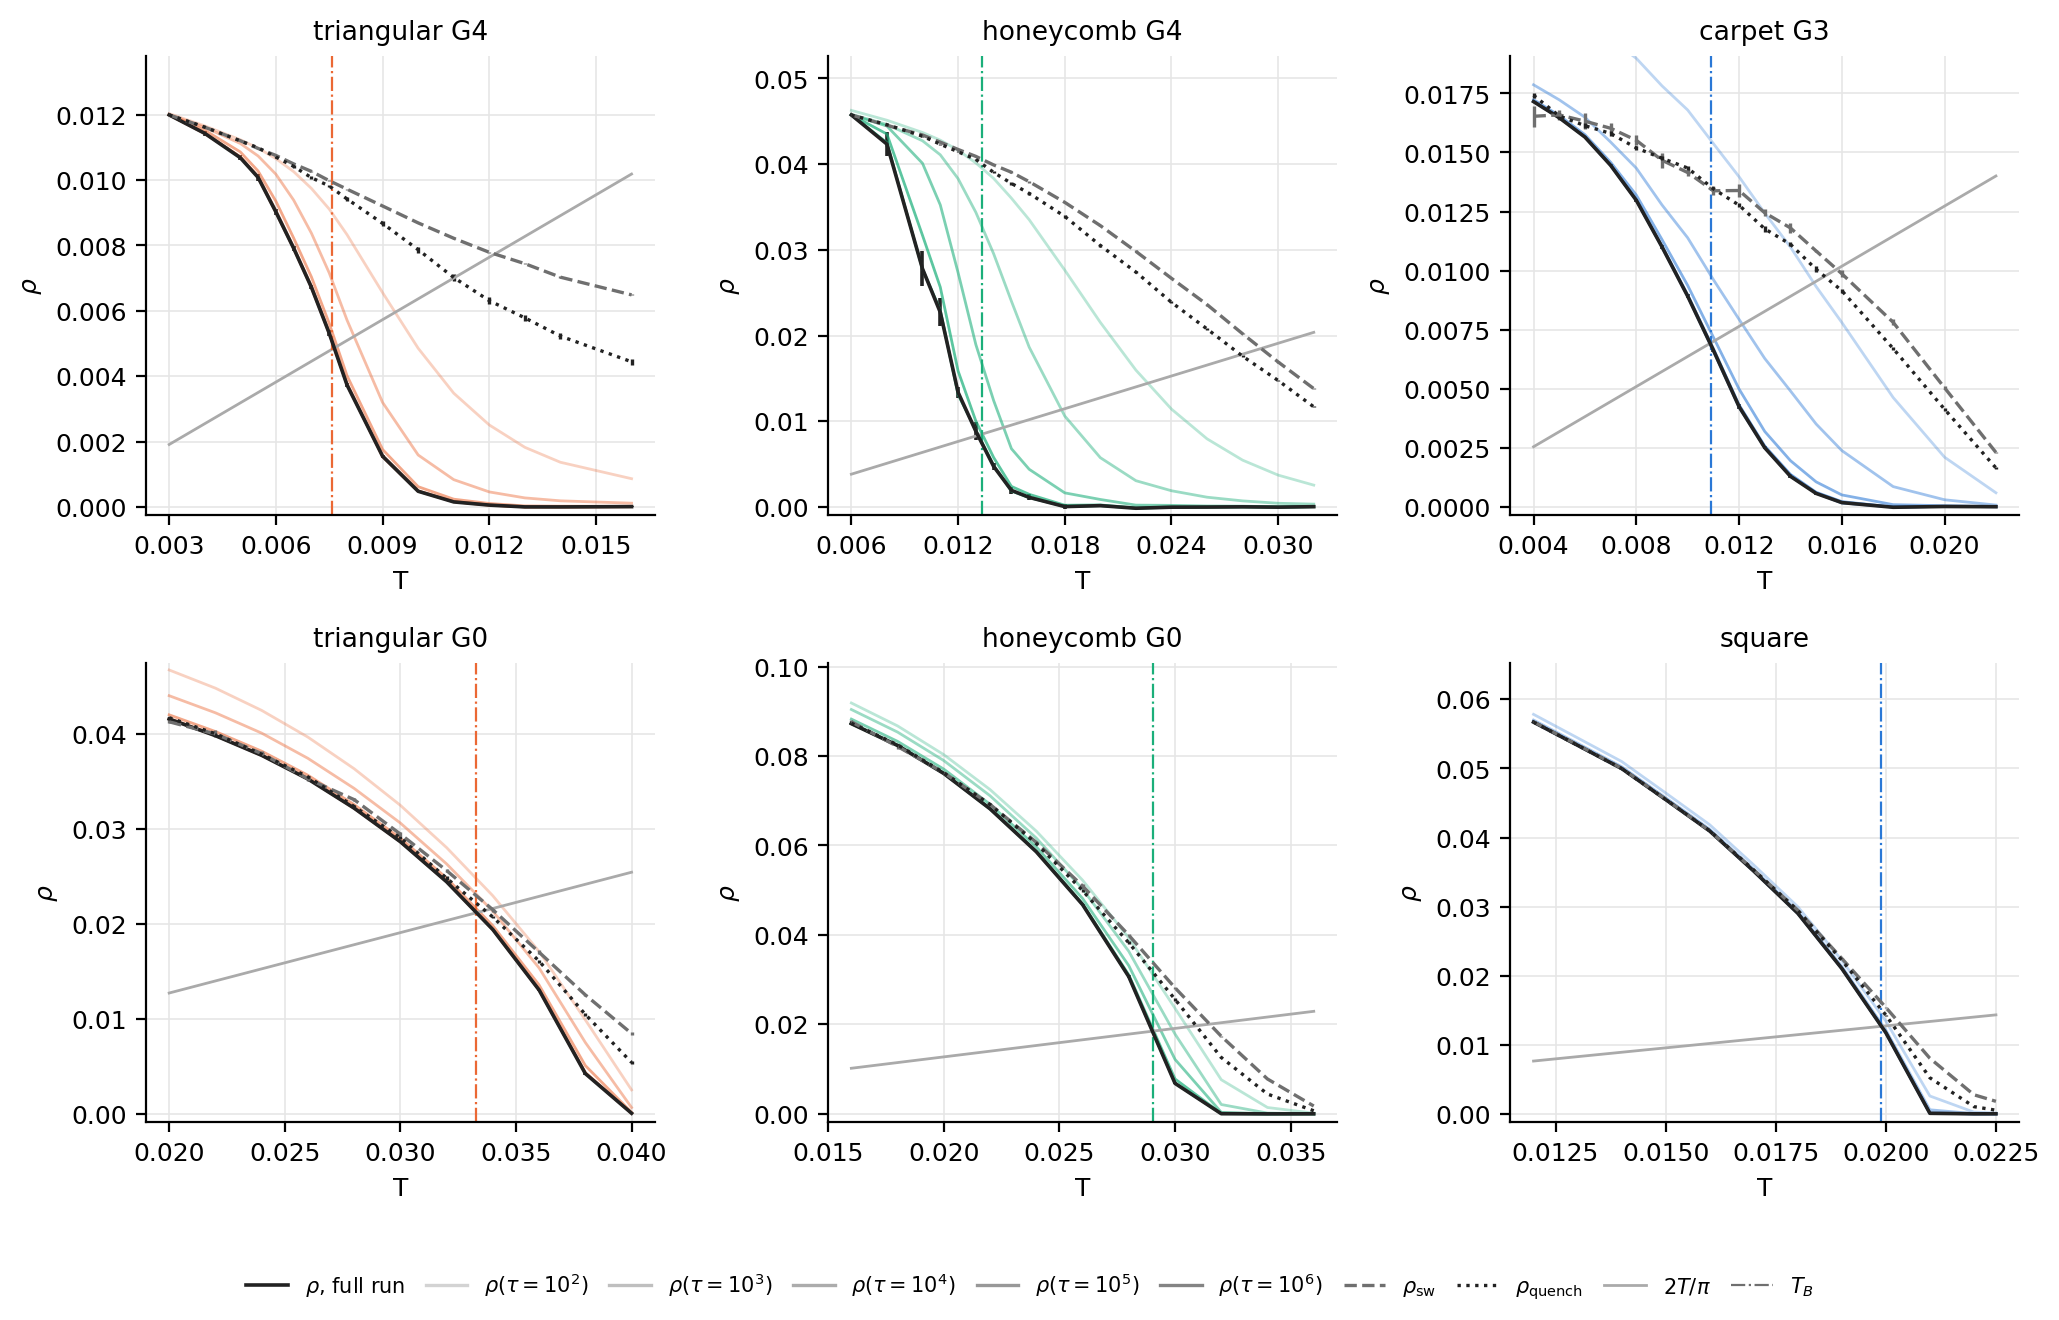
\includegraphics[width=0.95\textwidth]{vortex_stiffness_time.png}
\caption{Time-dependent two-terminal stiffness $\rho(T,\tau)$ evaluated over finite observation windows ranging from $\tau = 10^2$ to $10^6$ Monte Carlo sweeps at $U=1$ ($w=3$, Stage-1 BdG couplings), compared against the quenched-vortex limit $\rho_{\mathrm{quench}}(T)$ (thermal vortices frozen in place), the vortex-free spin-wave limit $\rho_{\mathrm{sw}}(T)$, and the BKT line $2T/\pi$. On the fractals, freezing the lacuna charges elevates the apparent crossover to $T_{\mathrm{quench}} \approx (1.4\text{--}2.1)\,T_B$, but vortex escape relaxes $\rho(T,\tau)$ back to equilibrium within $10^4\text{--}5\times 10^4$ sweeps.}
\label{fig:vortex_stiffness_time}
\end{figure*}

\begin{figure*}[htbp]
\centering
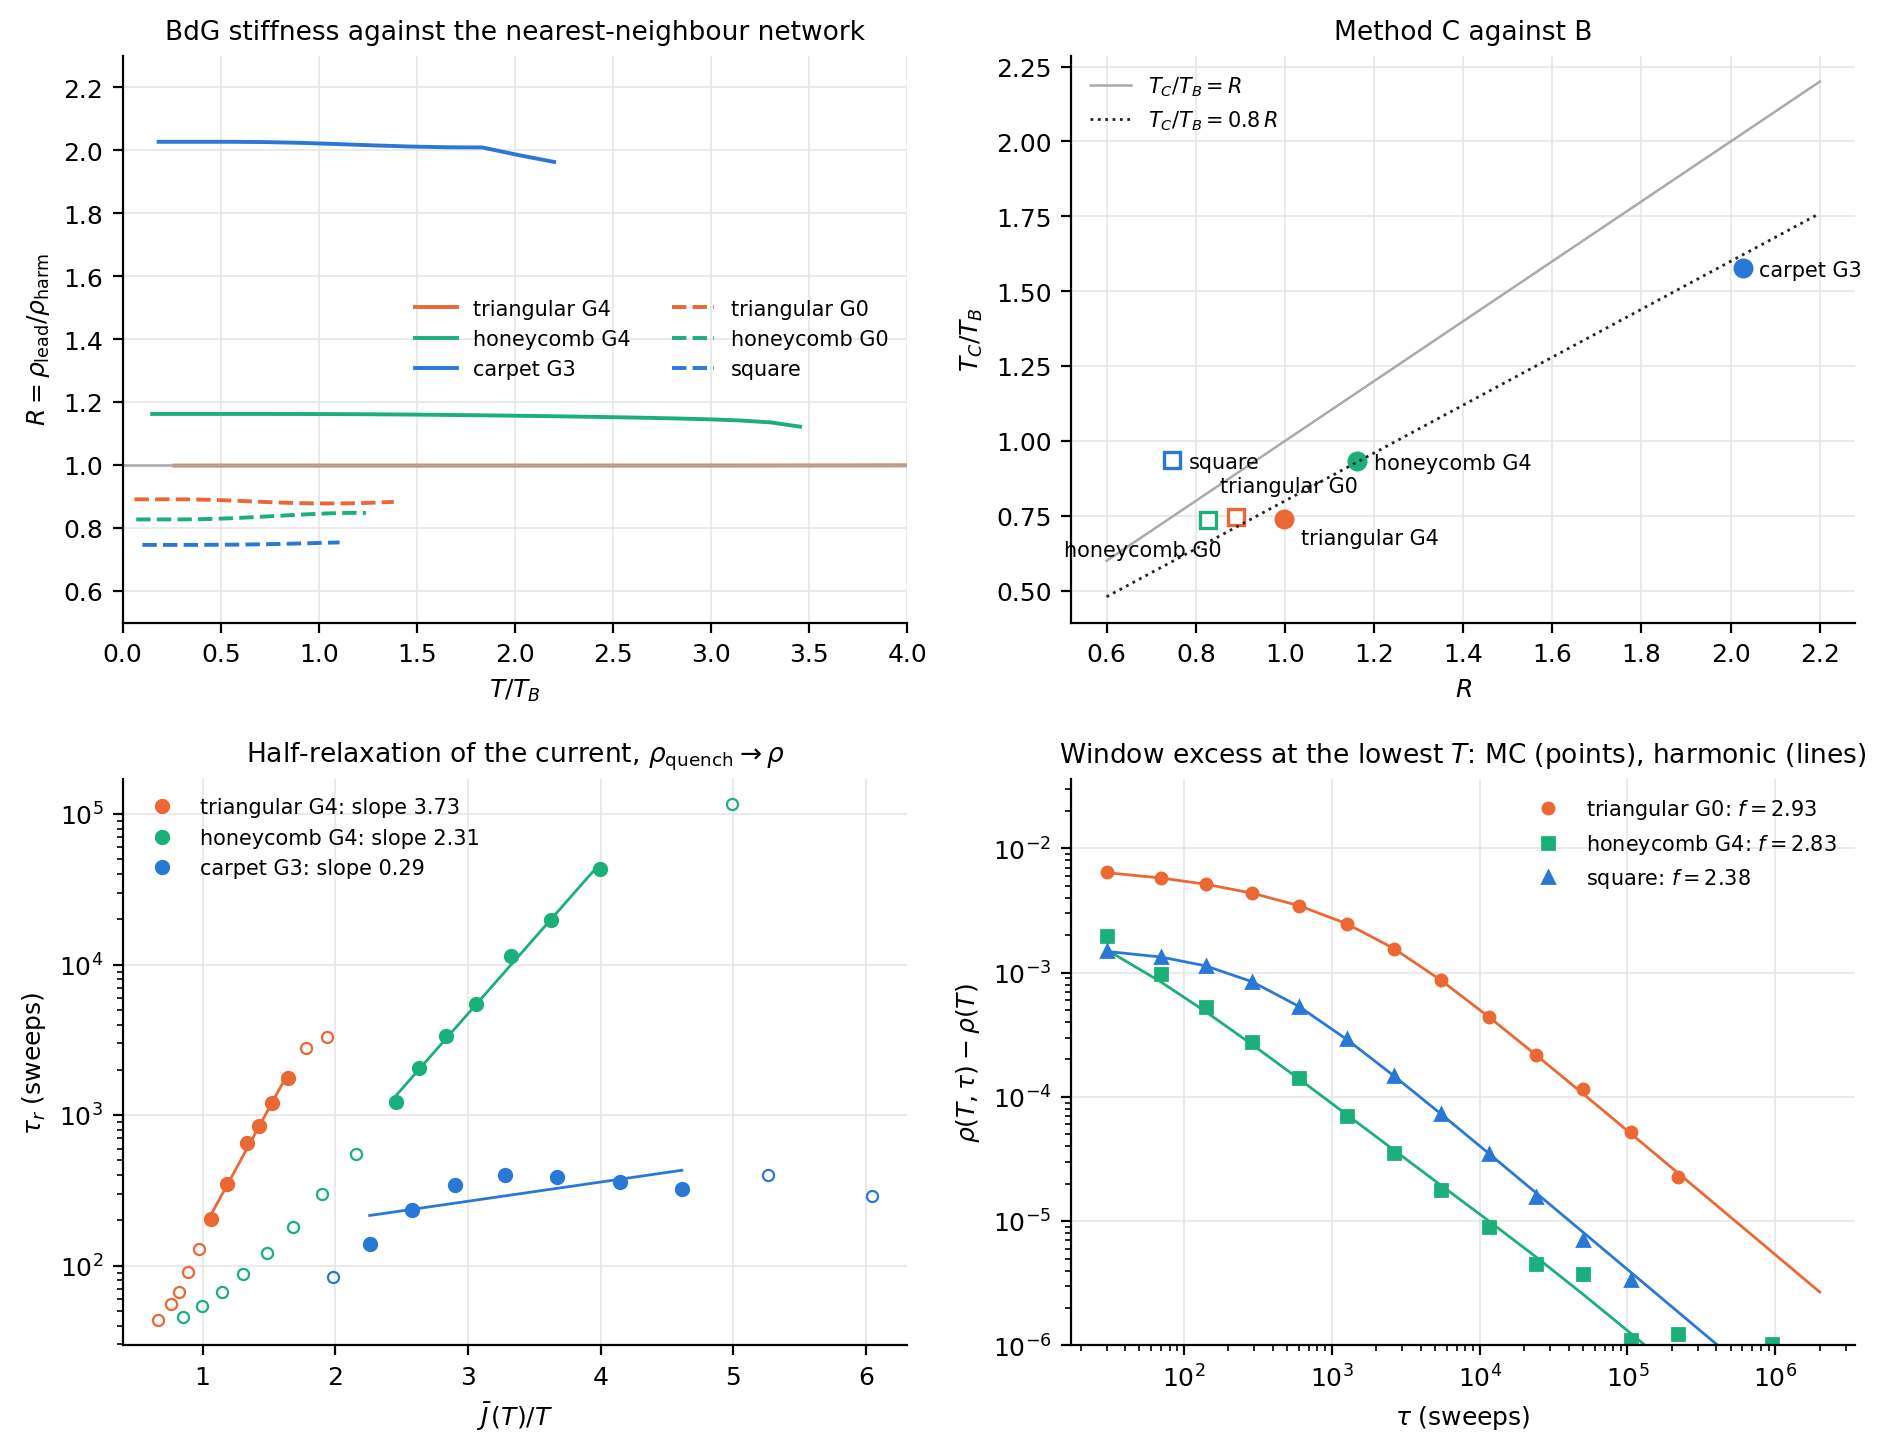
\includegraphics[width=0.92\textwidth]{vortex_scale_relaxation.png}
\caption{Stiffness scale ratios and current relaxation dynamics at $U=1$. Top left: temperature independence of the linear-response stiffness ratio $R(T) = \rlead/\rho_{\mathrm{harm}}$. Top right: ratio of full-BdG to XY crossover temperatures $T_{C0}/T_B$ versus $R$ (filled markers: fractals; open markers: filled parents). Bottom left: Arrhenius plot of the vortex-driven current relaxation time $\tau_r(T)$ versus $\bar{J}(T)/T$, whose fitted activation slopes match the static escape barrier $B_{\mathrm{esc}}$ of the largest central lacuna. Bottom right: low-temperature vortex-free window excess $\rho(T,\tau) - \rho(T)$ over four decades in $\tau$, fitted by the analytical harmonic spin-wave relaxation formula Eq.~\eqref{eq:spinwave_excess} to calibrate the dynamical time unit $f$.}
\label{fig:vortex_scale_relaxation}
\end{figure*}

To isolate the true vortex contribution to current decay from the trivial cutoff of slow harmonic spin waves by a short window $\tau$, we solve the overdamped Langevin dynamics of the vortex-free harmonic network analytically. Each normal mode $k$ of the free-site coupling Laplacian, with eigenvalue $w_k$ and macroscopic current overlap $c_k$, relaxes at rate $r_k = w_k / (6 J_{\mathrm{ref}} f)$ per sweep, producing an analytical spin-wave window excess
\begin{equation}
\rho_{\mathrm{sw}}(T,\tau) - \rho_{\mathrm{sw}}(T) = \frac{1}{g_0}\sum_k \frac{c_k^2}{w_k}\,g(r_k \tau), \qquad g(x) = \frac{2(x - 1 + e^{-x})}{x^2}.
\label{eq:spinwave_excess}
\end{equation}
As shown in the bottom-right panel of Fig.~\ref{fig:vortex_scale_relaxation}, fitting Eq.~\eqref{eq:spinwave_excess} with a single parameter $f$ to the lowest-temperature vortex-free Monte Carlo data reproduces the measured window excess over four decades in $\tau$ ($10^1\text{--}10^5$ sweeps), fixing the dynamical mobility factor $f$. Subtracting this exact spin-wave excess from $\rho(T,\tau)$ defines the vortex-driven current relaxation time $\tau_r(T)$ as the window duration at which the remaining vortex excess falls to half of its quenched value $\rho_{\mathrm{quench}}(T) - \rho(T)$.

The resulting relaxation dynamics (Table~\ref{tab:vortex_flakes} and Figs.~\ref{fig:vortex_stiffness_time} and~\ref{fig:vortex_scale_relaxation}) reveal the microscopic bottleneck of supercurrent decay on fractal networks:
\begin{enumerate}
\item \emph{Escape from the largest central lacuna is the rate-limiting step.} Near $T_B$, the current relaxation time $\tau_r(T)$ obeys an Arrhenius law with activation slope $3.73 \pm 0.14\,\bar{J}$ on the BdG triangular gasket and $2.31 \pm 0.07\,\bar{J}$ on the BdG honeycomb gasket (and $2.80 \pm 0.20\,J$ and $1.43 \pm 0.05\,J$ for uniform couplings). In every case, this dynamical activation energy agrees to within $3\%\text{--}15\%$ with the static escape barrier $B_{\mathrm{esc}}$ of the \emph{largest internal lacuna} ($3.85\,\bar{J}$ and $2.34\,\bar{J}$ for BdG couplings; $3.06\,J$ and $1.69\,J$ for uniform couplings), while lying well below both the exterior entry barrier of that lacuna ($5.38\,\bar{J}$ and $3.11\,\bar{J}$) and the full sample crossing barrier $E_{\mathrm{cross}}$ ($5.68\,\bar{J}$ and $3.07\,\bar{J}$). On the triangular gasket, boundary entry ($5.38\,\bar{J}$) and internal pair creation ($5.90\,\bar{J}$) are decisively excluded as the rate-limiting step: near $T_B$, thermal vortices are already present inside the deep central trap, and macroscopic current relaxation is governed by the thermal activation required to liberate a trapped vortex from the largest lacuna so that it can complete a phase slip across the remaining neck.
\item \emph{Lacuna pinning transiently boosts stiffness, but relaxes far too fast for dc protection.} Freezing a thermal vortex configuration in place substantially elevates the apparent crossover temperature on all three fractals ($T_{\mathrm{quench}}/T_B = 1.45$ on the triangular gasket, $2.09$ on the honeycomb gasket, and $1.40$ on the carpet, compared with just $1.01\text{--}1.06$ on the filled parent flakes where vortices are scarce below $T_B$), and freezing only the lacuna charges reproduces virtually the entire enhancement. However, because the escape barrier of even the deepest lacuna is at most $B_{\mathrm{esc}} \approx (2\text{--}4)\,\bar{J}$, the ratio $B_{\mathrm{esc}}/T_B \approx 3\text{--}8$ is vastly smaller than the factor $\ln(\nu t_{\mathrm{exp}}) \approx 25\text{--}30$ required for glassy arrest on laboratory timescales. As Fig.~\ref{fig:vortex_stiffness_time} demonstrates, $\rho(T,\tau)$ and $T_{\mathrm{obs}}(\tau)$ relax to within $2\%$ of their equilibrium values by $\tau \approx 1.0\times 10^4$ sweeps on the triangular gasket, $5.1\times 10^4$ sweeps on the honeycomb gasket, and $0.9\times 10^4$ sweeps on the carpet. Converting Monte Carlo sweeps to physical time via the resistively-shunted-junction (RSJ) time unit $\tau_0 = \hbar/(2e R_b I_0) \approx (1.03\,\mathrm{k\Omega}/R_b)\,\hbar/t$~\cite{AH69,HTB90} shows that one sweep corresponds to $(1.5\text{--}4.9)\,\tau_0$, so complete current equilibration occurs within $\sim 10^5\,\hbar/t$ (picoseconds to nanoseconds in typical solid-state or artificial arrays), many orders of magnitude shorter than any dc transport measurement.
\end{enumerate}

%----------------------------------------------------------------------
\subsection{Vortex metastability and barrier suppression in the full BdG functional}
\label{sec:vortex_bdg_barriers}
%----------------------------------------------------------------------

The vortex analysis above used the local XY energy Eq.~\eqref{eq:xy_coupled_graph}, which assumes that nearest-neighbor couplings $J_b(T)$ derived from infinitesimal uniform twists remain valid inside the strongly twisted core of a vortex and that the pairing amplitude $|\Delta_i|$ stays rigidly fixed as a vortex squeezes through a narrow fractal neck. To test both assumptions directly, we relax single-vortex states and minimum-energy escape strings inside the exact static-path BdG free-energy functional $F[\Delta]$ (Eq.~\eqref{eq:F_static_path}) at both $U=1$ (Table~\ref{tab:bdg_vortices_u1} and bottom panels of Fig.~\ref{fig:vortex_energies}) and $U=2$ (Table~\ref{tab:u2barriers}).

For each lacuna $f$ that holds a stable XY vortex, we initialize $\Delta_i = a_{0,i} e^{i\theta_i^{\mathrm{XY}}}$ and minimize $F[\Delta]$ via step-limited L-BFGS (so that a vortex can escape only along a monotonically downhill path in $F$), checking true local stability by computing the lowest non-trivial eigenvalue $\lambda$ of the full finite-difference BdG Hessian (excluding the global $\mathrm{U}(1)$ phase mode, which sits at $|\lambda_0| \le 3\times 10^{-5}$). Checking $\lambda > 0$ is indispensable on symmetric flakes: a vortex placed in the central lacuna shares the point-group symmetry of the entire fractal, so a gradient minimizer preserves its central position even when the state has turned into an unstable saddle point. For every genuinely metastable BdG vortex, we then initialize a simplified string along the optimal XY escape route to the exterior boundary and relax the trajectory on $F[\Delta]$ either with frozen amplitudes $|\Delta_i| = a_{0,i}$ (isolating the effect of the nonlocal, non-cosine phase kernel of Rung~P) or with both amplitudes and phases free (capturing the full amplitude-assisted escape of Rung~C).

\begin{table*}[htbp]
\caption{Vortex metastability, single-vortex creation energy $E_1$, exterior escape barrier $B_{\mathrm{out}}$, highest saddle point along the escape trajectory, and lowest non-trivial Hessian eigenvalue $\lambda$ in the full static-path BdG functional $F[\Delta]$ compared against the local XY model with Stage-1 couplings $J_b(T)$ at intermediate coupling $U=1$ (all energies in units of $\bar{J}(T)$). On the carpet at $T=0.010$, $\lambda < 0$ indicates that the central vortex has become a doubly degenerate symmetric saddle point with zero escape barrier. On the filled parent flakes (not listed), no vortex remains metastable in $F[\Delta]$.}
\label{tab:bdg_vortices_u1}
\begin{ruledtabular}
\begin{tabular}{lcccccccc}
 & & \multicolumn{2}{c}{$E_1$} & \multicolumn{2}{c}{$B_{\mathrm{out}}$} & \multicolumn{2}{c}{Highest saddle point} & Lowest Hessian \\
System & $P$ & XY & BdG & XY & BdG & XY & BdG & eigenvalue $\lambda$ \\
\hline
Triangular gasket $G=4$, $T=0.008$ & 6, 12 & \multicolumn{7}{c}{No metastable vortex in $F[\Delta]$ (escapes with zero barrier)} \\
 & 24 & 2.76 & 2.67 & 3.06 & 0.19 & 5.82 & 2.86 & $+0.0039$ \\
 & 48 & 1.53 & 1.54 & 3.85 & 0.82 & 5.38 & 2.36 & $+0.0039$ \\
\hline
Honeycomb gasket $G=4$, $T=0.014$ & 6, 12, 24 & \multicolumn{7}{c}{No metastable vortex in $F[\Delta]$ (escapes with zero barrier)} \\
 & 48 & 0.89 & 1.12 & 2.15 & 0.25 & 3.04 & 1.37 & $+0.0108$ \\
 & 96 & 0.51 & 0.64 & 2.60 & 0.83 & 3.11 & 1.47 & $+0.0107$ \\
\hline
Sierpi\'nski carpet $G=3$, $T=0.010$ & 6--28 & \multicolumn{7}{c}{No metastable vortex in $F[\Delta]$ (escapes with zero barrier)} \\
 & 40 & 0.78 & 1.76 & 0.95 & 0.00 & 1.73 & 1.76 & $-0.0058$ \\
\hline
Sierpi\'nski carpet $G=3$, $T=0.004$ & 6--24 & \multicolumn{7}{c}{No metastable vortex in $F[\Delta]$ (escapes with zero barrier)} \\
 & 40 & 0.79 & 1.96 & 0.95 & 0.06 & 1.74 & 2.02 & $+0.0573$ \\
\end{tabular}
\end{ruledtabular}
\end{table*}

\begin{table*}[htbp]
\caption{Three-rung comparison of single-vortex energies $E_1$ and exterior escape barriers $B_{\mathrm{out}}$ (in units of $\bar{J}(T)$) at strong coupling $U=2$ across the local XY model with $J_b(T)$ (Rung~B), the frozen-amplitude BdG functional $F[a_0 e^{i\theta}]$ (Rung~P), and the full amplitude-and-phase BdG functional $F[\Delta]$ (Rung~C). Here $n$ denotes the number of lacunae of perimeter $P$ that retain a metastable vortex minimum in the corresponding functional (out of $9, 3, 1$ tried on the gaskets and $8, 8, 1$ on the carpet for the three largest perimeter classes). Ranges reflect path differences across symmetry-equivalent faces.}
\label{tab:u2barriers}
\begin{ruledtabular}
\begin{tabular}{lccccccc}
 & & \multicolumn{2}{c}{XY with $J_b$ (Rung B)} & \multicolumn{2}{c}{BdG frozen amp.\ (Rung P)} & \multicolumn{2}{c}{BdG full (Rung C)} \\
System & $P$ & $E_1$ & $B_{\mathrm{out}}$ & $n$, $E_1$ & $B_{\mathrm{out}}$ & $n$, $E_1$ & $B_{\mathrm{out}}$ \\
\hline
Triangular gasket $G=4$, $T=0.0245$ & 12 & 4.74 & 1.70 & 9, 4.98 & 0.75--0.95 & 3, 4.33 & 0.01--1.74 \\
 & 24 & 2.74 & 2.99 & 3, 2.87 & 2.04 & 3, 2.81 & 0.59--1.33 \\
 & 48 & 1.55 & 3.82 & 1, 1.63 & 2.90 & 1, 1.62 & 1.34 \\
\hline
Sierpi\'nski carpet $G=3$, $T=0.0511$ & 8 & 5.07 & 0.97 & 4, 4.13 & 0.60--0.62 & 0, \phantom{0.0}-- & -- \\
 & 16 & 2.93 & 1.73 & 8, 3.04 & 0.52--0.56 & 8, 3.02 & 0.11--0.24 \\
 & 40 & 1.96 & 3.51 & 1, 1.97 & 2.68 & 1, 1.97 & 2.17 \\
\hline
Honeycomb gasket $G=4$, $T=0.0285$ & 24 & 1.47 & 1.54 & 9, 1.76 & 0.35--0.42 & 9, 1.74 & 0.24--1.68 \\
 & 48 & 0.84 & 1.99 & 3, 1.01 & 0.81--0.83 & 3, 1.00 & 0.68--1.08 \\
 & 96 & 0.47 & 2.25 & 1, 0.57 & 1.12 & 1, 0.57 & 1.45 \\
\end{tabular}
\end{ruledtabular}
\end{table*}

Tables~\ref{tab:bdg_vortices_u1} and~\ref{tab:u2barriers} uncover two profound microscopic effects that distinguish a fermionic fractal superconductor from a rigid-spin XY array:
\begin{enumerate}
\item \emph{The nonlocal fermionic phase kernel washes out small-scale Peierls barriers.} Even when the pairing amplitudes are held rigidly frozen at $a_{0,i}$ (Rung~P), replacing the nearest-neighbor cosine potential by the exact fermionic phase functional $F[a_0 e^{i\theta}]$ eliminates vortex metastability in all elementary plaquettes and on the filled open parent flakes (where an XY vortex has energy $9\text{--}25\,\bar{J}$ and is locally pinned by the lattice Peierls barrier, yet slides smoothly out of the open BdG flake with zero barrier because a vortex core broader than one lattice spacing averages over the discrete bond periodicity). On the fractals at $U=1$, the exact kernel alone destabilizes all non-central lacunae on the carpet; only the central $P=40$ hole retains a minimum at very low temperature ($\lambda = +0.0573$ at $T=0.004$), and its doubly degenerate translational Hessian eigenvalue crosses zero at $T \approx 0.0096$ ($\lambda = -0.0058$ at $T=0.010$), turning the central vortex into a symmetric saddle point so that no metastable vortex exists anywhere on the carpet near $T_B = 0.0109$ or $T_{C0} = 0.0172$. At $U=2$, where the kernel is shorter-ranged, the three largest lacuna classes ($P=12,24,48$ on triangular $G=4$; $P=24,48,96$ on honeycomb $G=4$; $P=8,16,40$ on carpet $G=3$) remain metastable in the frozen-amplitude functional, and their single-vortex creation energies $E_1$ agree closely with the XY model (after accounting for the stiffness scale ratio $R$), confirming that far from a bond crossing a lacuna-trapped vortex is primarily a long-wavelength phase winding. Even at $U=2$, however, the non-cosine flattening of the exact phase kernel at large bond angles lowers the frozen-amplitude escape barrier $B_{\mathrm{out}}$ below the XY value across every single lacuna size by a factor of $1.3\text{--}4$ (Table~\ref{tab:u2barriers}).
\item \emph{Local amplitude softening in narrow necks collapses the escape barrier.} Allowing the pairing amplitudes $|\Delta_i|$ to relax along the escape trajectory in the full functional $F[\Delta]$ (Rung~C) produces a dramatic further reduction of vortex trapping. At $U=1$ (Table~\ref{tab:bdg_vortices_u1}), smaller gasket lacunae ($P=12$ on the triangular gasket and $P=24$ on the honeycomb gasket, which remained stable under frozen amplitudes) lose metastability altogether once amplitudes can deform, leaving only the two largest hole tiers ($P \ge 24$ on triangular and $P \ge 48$ on honeycomb) able to trap a vortex. In those surviving traps, the exterior escape barrier $B_{\mathrm{out}}$ plummets by a factor of $3\text{--}16$ relative to the XY model (falling from $3.06$ and $3.85\,\bar{J}$ down to $0.19$ and $0.82\,\bar{J}$ on the triangular gasket, and from $2.15$ and $2.60\,\bar{J}$ down to $0.25$ and $0.83\,\bar{J}$ on the honeycomb gasket). At $U=2$ (Table~\ref{tab:u2barriers}), amplitude relaxation similarly destabilizes all $P=8$ carpet holes and six of the nine $P=12$ triangular holes, while reducing $B_{\mathrm{out}}$ of the central triangular ($P=48$) and carpet ($P=40$) lacunae to $1.34\,\bar{J}$ and $2.17\,\bar{J}$, respectively (noting that on several smaller symmetry-equivalent faces at $U=2$, the high-dimensional full-BdG string converges to distinct local path classes, making the quoted full-BdG barriers path-dependent upper bounds). Inspection of the order-parameter profile at the saddle point of the string reveals the physical mechanism of this collapse: as the vortex core squeezes across a single-site articulation neck or thin inter-lacuna wall, the local pairing modulus $|\Delta_i|$ on the bottleneck site softens to $20\%\text{--}45\%$ of its vacuum value $a_{0,i}$. Rather than paying the full exchange cost $2 J_b$ of rotating two rigid spins through $\pi$ across a bottleneck bond, the fermionic condensate momentarily suppresses the local gap amplitude on a single articulation vertex, allowing the vortex to slip out of the lacuna through a self-induced weak link.
\end{enumerate}

%======================================================================
\section{Discussion and Conclusions}
\label{sec:discussion}
%======================================================================

Taken together with recent mean-field studies of pairing on fractal lattices~\cite{Iliasov2024,Canyellas2026dwave} and variational neural-quantum-state calculations of the zero-temperature quantum rotor limit~\cite{Canyellas2026quantum}, the four-rung thermal hierarchy developed in this work completes a unified physical picture of superconductivity on regular fractal structures across energy, length, and temperature scales.

At the single-particle and mean-field level, recursive excision of a crystal into a finitely ramified fractal such as the Sierpi\'nski gasket compresses the electronic spectrum into narrow, highly degenerate sub-clusters and confines the anomalous pairing correlator to the single-bond scale ($\xi_{\mathrm{pair}} \sim 1$). At weak to intermediate attraction ($U=1$), this spectral pileup strongly enhances the local pairing amplitude and nearly doubles the mean-field pair-formation temperature $\Tmf$ relative to the pristine parent lattice~\cite{Iliasov2024}, while reshaping the competition between unconventional pairing symmetries~\cite{Canyellas2026dwave}. A natural concern is whether zero-point quantum phase fluctuations in such a low-dimensional, poorly connected network immediately destroy off-diagonal order even at $T=0$. The spin-$1/2$ quantum XY study of Ref.~\cite{Canyellas2026quantum} settled that question in the negative: even in the extreme quantum limit of at most one Cooper pair per site ($E_C \gg E_J$), quantum fluctuations leave algebraic quasi-long-range order ($C_{xy}(r) \sim r^{-\eta}$ with $\eta \simeq 0.12\text{--}0.32$) intact across all accessible gasket generations.

The decisive bottleneck for fractal superconductivity therefore lies entirely in the classical, finite-temperature phase sector analyzed here. On a finitely ramified gasket, the very same geometric bottlenecks—corner articulation sites of coordination $z=4$ and a self-similar hierarchy of open lacunae—that localize the electronic states and elevate $\Tmf$ simultaneously choke the macroscopic two-terminal phase stiffness and bound the energy cost of a topological defect. Because an arbitrarily large triangular or honeycomb gasket block can be severed by cutting a finite number of corner bonds, the single-vortex creation energy in the largest lacunae ($E_1 \propto P^{-0.8}$) and the macroscopic phase-slip crossing barrier ($E_{\mathrm{cross}} \approx 4\text{--}6\,\bar{J}$) saturate to small, generation-independent constants instead of growing logarithmically with system size as in two Euclidean dimensions. Furthermore, while the large internal lacunae act as topological traps whose static saddle barriers $B_{\mathrm{esc}}$ govern the Arrhenius activation of the supercurrent relaxation time $\tau_r(T)$ near the BKT crossover, those barriers are at most a few $\bar{J}$—and are lowered still further, by up to an order of magnitude, when the fermionic condensate softens its local amplitude $|\Delta_i|$ to let a vortex slip through a narrow bottleneck site. As a result, pinned vortices equilibrate within $\sim 10^4\text{--}5\times 10^4$ Monte Carlo sweeps ($\sim 10^5\,\hbar/t$), far too fast to arrest dissipation on laboratory dc timescales. Thermal phase fluctuations consequently drive the finite-size BKT crossover temperature $T_C$ down by an order of magnitude below $\Tmf$ and a factor of $2\text{--}5$ below the pristine parent crystal, opening a broad pseudogap-like regime of preformed, incoherent Cooper pairs and causing the crossover temperature to decay with generation at the universal power-law rate $T^*(G) \propto L^{-x}$ ($x \approx 0.50\text{--}0.56$) on its way to zero in the thermodynamic limit~\cite{GMA80,GAM83,Vallat1991,MB10}.

From a methodological standpoint, our four-rung ladder (A $\to$ B $\to$ P $\to$ C) establishes clear criteria for when effective spin mappings of inhomogeneous superconductors can be trusted and when full fermionic sampling is required:
\begin{enumerate}
\item \emph{When the local XY mapping succeeds:} On finitely ramified gaskets, fractal confinement compresses the Cooper-pair radius $\xi_{\mathrm{pair}}$ and the phase-kernel range $\xi_K$ to the lattice constant, concentrating up to $71\%$ of the phase kernel onto nearest-neighbor bonds. Under these conditions, Pippard contact losses vanish even for single-bond leads, and the nearest-neighbor XY model with temperature-dependent BdG couplings $J_b(T)$ (Rung~B) reproduces the BKT crossover temperature of the full static-path BdG functional (Rungs~P and~C) to within $\sim 15\%$.
\item \emph{When the local XY mapping breaks down:} On two-dimensional filled crystals and infinitely ramified fractals such as the Sierpi\'nski carpet, two distinct failures occur. First, at weak-to-intermediate coupling where $\xi_{\mathrm{pair}}$ spans many lattice sites, Pippard nonlocality allows an imposed phase twist to slip across narrow contacts ($w \lesssim \xi_{\mathrm{pair}}$), while projecting the long-range phase kernel onto nearest neighbors generates frustrated negative couplings $J_b < 0$ around sharp geometric corners on the carpet. Second, even at strong coupling ($U=2$) where $\xi_{\mathrm{pair}} \approx 2$, negative couplings vanish, and linear-response stiffness scales match ($R \approx 1$), the nearest-neighbor cosine model overestimates the true fermionic BKT crossover by a factor of $1.3\text{--}2.0$ because it misses the non-cosine flattening of the fermionic phase energy at large angles and the reduced core cost of extended fermionic vortices. At the same time, allowing thermal amplitude fluctuations ($P \to C$) systematically \emph{raises} the phase-coherence crossover on the carpet and filled lattices by $13\%\text{--}29\%$ via thermal enhancement of the mean-square gap $\langle |\Delta|^2 \rangle$.
\end{enumerate}

Finally, our results clarify the practical design rules for artificial superconducting nanostructures—whether assembled atom-by-atom via scanning tunneling microscopy~\cite{Kempkes2019,Canyellas2024Bi}, synthesized by molecular self-assembly~\cite{Shang2015,Li2017}, or patterned as mesoscopic lithographic networks~\cite{Gordon1986,Meyer1991,Meyer2002}—which are always of finite generation $G$ by construction. On a strictly self-similar gasket, increasing the generation $G$ sharpens the spectral clustering that promotes pair formation, but progressively degrades the macroscopic phase stiffness and lowers the BKT crossover as $2^{-xG}$, confining useful superconducting coherence to low generation orders. Overcoming this finitely ramified trade-off points toward a clear geometric principle for engineered superconducting metamaterials: to harness the spectral localization and boundary-induced pairing enhancements of perforated lattices without suffering catastrophic phase-stiffness collapse or amplitude-assisted vortex slip, one must eliminate single-site articulation bottlenecks ($z=4$ corner vertices and single-bond bridges) and instead preserve multi-bond, high-coordination ($z=6$) current highways around compact, well-separated internal lacunae.

%======================================================================
\begin{acknowledgments}
The work of R.C., M.I.K., and A.A.B. was supported by the research program ``Materials for the Quantum Age'' (QuMat, registration number 024.005.006), which is part of the Gravitation program financed by the Dutch Ministry of Education, Culture and Science (OCW). A.A.B. and M.I.K. also acknowledge support from the European Research Council (ERC) under the European Union's Horizon 2020 research and innovation program, Grant Agreement No.~854843-FASTCORR, and A.A.B. was supported by NWO Grant No.~OCENW.M.23.044.
\end{acknowledgments}

\appendix

\section{Mapping the Attractive Hubbard Model to the Phase Hessian}
\label{app:hessian}

In this Appendix we present the complete derivation connecting the microscopic attractive Hubbard Hamiltonian to the quadratic bond-phase and site-phase Hessians used in Section~\ref{sec:model}.

\subsection{Imaginary-time action and Hubbard--Stratonovich decoupling}

In the grand-canonical ensemble, the attractive Hubbard Hamiltonian takes the form
\begin{equation}
\hat{H} - \mu \hat{N} = \sum_{ij}\sum_{\sigma\sigma'} \hat{c}_{i\sigma}^\dagger h_{ij}^{\sigma\sigma'} \hat{c}_{j\sigma'} - U \sum_i \hat{n}_{i\uparrow}\hat{n}_{i\downarrow}, \qquad U > 0,
\label{eq:A1}
\end{equation}
where the one-particle matrix $h_{ij}^{\sigma\sigma'}$ contains the chemical potential and may also incorporate hopping, on-site Hartree shifts, disorder, Zeeman fields, or spin--orbit coupling. The grand-canonical partition function is given by the functional integral over Grassmann fields $(\bar{c}, c)$,
\begin{equation}
Z = \Tr e^{-\beta(\hat{H}-\mu\hat{N})} = \int \mathcal{D}[\bar{c},c]\, e^{-S[\bar{c},c]},
\label{eq:A2}
\end{equation}
with Euclidean action
\begin{equation}
S[\bar{c},c] = \int_0^\beta d\tau \left[ \sum_{ij}\sum_{\sigma\sigma'} \bar{c}_{i\sigma}\left(\delta_{ij}\delta_{\sigma\sigma'}\partial_\tau + h_{ij}^{\sigma\sigma'}\right)c_{j\sigma'} - U\sum_i \bar{c}_{i\uparrow}\bar{c}_{i\downarrow}c_{i\downarrow}c_{i\uparrow} \right],
\label{eq:A3}
\end{equation}
where $\beta = (k_B T)^{-1}$.

Introducing a complex auxiliary Hubbard--Stratonovich pairing field $\Delta_i(\tau)$ on each lattice site decouples the quartic attraction. Up to a field-independent normalization factor $\mathcal{N}$,
\begin{equation}
\exp\left[ U \int_0^\beta d\tau\, \bar{c}_{i\uparrow}\bar{c}_{i\downarrow}c_{i\downarrow}c_{i\uparrow} \right] = \mathcal{N} \int \mathcal{D}[\Delta_i,\Delta_i^*] \exp\left\{ -\int_0^\beta d\tau \left[ \frac{|\Delta_i|^2}{U} - \Delta_i \bar{c}_{i\uparrow}\bar{c}_{i\downarrow} - \Delta_i^* c_{i\downarrow}c_{i\uparrow} \right] \right\}.
\label{eq:A4}
\end{equation}
The partition function then becomes
\begin{equation}
Z = \int \mathcal{D}[\bar{c},c,\Delta,\Delta^*]\, e^{-S_{\mathrm{HS}}},
\label{eq:A5}
\end{equation}
with the Hubbard--Stratonovich action
\begin{equation}
S_{\mathrm{HS}} = \int_0^\beta d\tau \left[ \sum_{ij}\sum_{\sigma\sigma'} \bar{c}_{i\sigma}\left(\delta_{ij}\delta_{\sigma\sigma'}\partial_\tau + h_{ij}^{\sigma\sigma'}\right)c_{j\sigma'} + \sum_i \frac{|\Delta_i|^2}{U} - \sum_i \left(\Delta_i \bar{c}_{i\uparrow}\bar{c}_{i\downarrow} + \Delta_i^* c_{i\downarrow}c_{i\uparrow}\right) \right].
\label{eq:A6}
\end{equation}

\subsection{Integrating out the fermions and the mean-field grand potential}

The fermionic part of Eq.~\eqref{eq:A6} can be cast into quadratic form by introducing the doubled Nambu--Grassmann basis $\Psi_i = (c_{i\uparrow}, c_{i\downarrow}, \bar{c}_{i\uparrow}, \bar{c}_{i\downarrow})^T$. In terms of this enlarged field, the fermionic action reads
\begin{equation}
S_F = -\frac{1}{2} \bar{\Psi}\, G^{-1}[\Delta]\, \Psi,
\label{eq:A7}
\end{equation}
where $G^{-1}[\Delta]$ is the inverse Nambu Green's function in the doubled Bogoliubov--de Gennes (BdG) space. Integrating out the Grassmann variables exactly via the Gaussian integral yields
\begin{equation}
\int \mathcal{D}[\bar{c},c]\, e^{-S_F} = \exp\left( \frac{1}{2}\Tr\ln\left[-G^{-1}[\Delta]\right] \right),
\label{eq:A8}
\end{equation}
up to field-independent normalization and normal-ordering contributions. Consequently, the partition function reduces to an integral over the pairing field alone,
\begin{equation}
Z = \int \mathcal{D}[\Delta,\Delta^*]\, e^{-S_{\mathrm{eff}}[\Delta,\Delta^*]},
\label{eq:A9}
\end{equation}
governed by the effective bosonic action
\begin{equation}
S_{\mathrm{eff}}[\Delta,\Delta^*] = \int_0^\beta d\tau \sum_i \frac{|\Delta_i|^2}{U} - \frac{1}{2}\Tr\ln\left[-G^{-1}[\Delta]\right] + S_{\mathrm{const}}.
\label{eq:A10}
\end{equation}

The mean-field configuration corresponds to the static saddle point $\Delta_i(\tau) = \Delta_i^{(0)}$, determined by the stationarity condition
\begin{equation}
\left.\frac{\delta S_{\mathrm{eff}}}{\delta \Delta_i^*(\tau)}\right|_{\Delta=\Delta^{(0)}} = 0 \implies \Delta_i^{(0)} = U \langle c_{i\downarrow}c_{i\uparrow} \rangle_{\mathrm{BdG}}.
\label{eq:A11}
\end{equation}
At leading saddle-point order, the partition function and mean-field grand potential are
\begin{equation}
Z_{\mathrm{MF}} \simeq e^{-S_{\mathrm{eff}}[\Delta^{(0)}]}, \qquad \Omega_{\mathrm{MF}} = \frac{1}{\beta} S_{\mathrm{eff}}[\Delta^{(0)}].
\label{eq:A12}
\end{equation}
For a static saddle-point configuration, we define the frequency-space inverse propagator
\begin{equation}
G_0^{-1}(i\omega_n) = i\omega_n - H_{\mathrm{BdG}}^{(0)}, \qquad H_{\mathrm{BdG}}^{(0)} \equiv H_{\mathrm{BdG}}[\Delta^{(0)}],
\label{eq:A13}
\end{equation}
where $G_0$ denotes the superconducting BdG Green's function evaluated at the self-consistent saddle point (rather than the bare normal-state propagator). Exploiting particle--hole symmetry of the doubled BdG spectrum and performing the Matsubara frequency summation yields the standard mean-field grand potential
\begin{equation}
\Omega_{\mathrm{MF}} = \sum_i \frac{|\Delta_i^{(0)}|^2}{U} - \frac{1}{\beta}\sum_{E_\nu > 0} \ln\left[2\cosh\left(\frac{\beta E_\nu}{2}\right)\right] + \Omega_{\mathrm{const}}.
\label{eq:A14}
\end{equation}
Here $\Omega_{\mathrm{const}}$ collects the normal-ordering trace $\Tr h_\downarrow$ and the Hartree double-counting terms $U\sum_i n_{i\uparrow}n_{i\downarrow}$ required by the self-consistent decoupling. While these constants are essential when comparing absolute grand potentials of competing saddle points, they are independent of the Peierls bond phases when the density is held fixed and therefore drop out of the quadratic phase-response derivatives below.

\subsection{Phase-only approximation and gauge rotation}

At the mean-field level, the amplitude of the superconducting order parameter is fixed self-consistently by the gap equation~\eqref{eq:A11}. To establish global superconducting order, however, the Cooper-pair condensate must maintain macroscopic phase coherence against thermal fluctuations. In the phase-only approximation, the pairing amplitude is frozen at its self-consistent real saddle-point value $\Delta_i^{(0)}$, while the local pair phases $\theta_i(\tau)$ are allowed to fluctuate:
\begin{equation}
\Delta_i(\tau) = \Delta_i^{(0)} e^{i\theta_i(\tau)}.
\label{eq:A15}
\end{equation}
To expand the effective action to second order in spatial phase gradients, we perform a local gauge transformation in Nambu space,
\begin{equation}
U_i(\tau) = \exp\left[ \frac{i}{2}\theta_i(\tau)(\tau_3 \otimes \sigma_0) \right],
\label{eq:A16}
\end{equation}
where $\tau_3$ and $\sigma_0$ act in particle--hole and spin spaces, respectively. This unitary rotation removes the phase from the on-site pairing matrix, transferring the phase dependence to the temporal derivative and the intersite hopping amplitudes:
\begin{align}
\partial_\tau &\longrightarrow \partial_\tau + \frac{i}{2}\dot{\theta}_i \tau_3, \label{eq:A17} \\
-t_{ij} &\longrightarrow -t_{ij} \exp\left[ -\frac{i}{2}\tau_3(\theta_i - \theta_j) \right]. \label{eq:A18}
\end{align}
In the static classical limit ($\dot{\theta}_i = 0$), only the spatial bond phase differences survive.

In the presence of an external electromagnetic vector potential $\bm{A}$, the gauge-invariant Cooper-pair phase difference across an oriented bond $b = (i \to j)$ is
\begin{equation}
\varphi_b = \theta_i - \theta_j - A_{ij}^{(2e)}, \qquad A_{ij}^{(2e)} = \frac{2e}{\hbar}\int_i^j \bm{A}\cdot d\bm{\ell},
\label{eq:A19}
\end{equation}
where $e > 0$ is the elementary charge. Because individual electrons carry charge $e$, the corresponding electronic Peierls phase entering the single-particle hopping matrix is half the Cooper-pair phase difference,
\begin{equation}
\alpha_b = \frac{\varphi_b}{2} = \frac{1}{2}(\theta_i - \theta_j) - \frac{e}{\hbar}\int_i^j \bm{A}\cdot d\bm{\ell}.
\label{eq:A20}
\end{equation}
In Nambu space, the hopping matrix on bond $b$ therefore carries the factor $e^{-i\tau_3 \alpha_b}$. At zero external magnetic field, the electronic bond phase reduces to
\begin{equation}
\alpha_b = \frac{1}{2}(\theta_i - \theta_j).
\label{eq:A21}
\end{equation}

\subsection{Expansion of the BdG Hamiltonian in bond phases}

We now expand the gauge-rotated BdG Hamiltonian around the untwisted saddle point $H_{\mathrm{BdG}}^{(0)}$,
\begin{equation}
H_{\mathrm{BdG}}(\alpha) = H_{\mathrm{BdG}}^{(0)} + \delta H_{\mathrm{BdG}}(\alpha).
\label{eq:A22}
\end{equation}
Defining the first- and second-order bond-current vertices
\begin{equation}
V_b = \left.\frac{\partial H_{\mathrm{BdG}}}{\partial \alpha_b}\right|_{\alpha=0}, \qquad W_{bb'} = \left.\frac{\partial^2 H_{\mathrm{BdG}}}{\partial \alpha_b \partial \alpha_{b'}}\right|_{\alpha=0},
\label{eq:A23}
\end{equation}
the perturbation expands as
\begin{equation}
\delta H_{\mathrm{BdG}}^{(1)} = \sum_b \alpha_b V_b, \qquad \delta H_{\mathrm{BdG}}^{(2)} = \frac{1}{2}\sum_{bb'} \alpha_b \alpha_{b'} W_{bb'},
\label{eq:A24}
\end{equation}
so that
\begin{equation}
H_{\mathrm{BdG}}(\alpha) = H_{\mathrm{BdG}}^{(0)} + \delta H_{\mathrm{BdG}}^{(1)} + \delta H_{\mathrm{BdG}}^{(2)} + \mathcal{O}(\alpha^3).
\label{eq:A25}
\end{equation}

Since the full inverse Green's function satisfies
\begin{equation}
G^{-1}(i\omega_n, \alpha) = i\omega_n - H_{\mathrm{BdG}}(\alpha),
\label{eq:A26}
\end{equation}
Dyson's equation takes the form
\begin{equation}
G^{-1} = G_0^{-1} - \delta H_{\mathrm{BdG}}.
\label{eq:A27}
\end{equation}
Expanding the fermionic functional determinant to second order in $\delta H_{\mathrm{BdG}}$ gives
\begin{align}
-\frac{1}{2}\Tr\ln\left[-G^{-1}\right] &= -\frac{1}{2}\Tr\ln\left[-G_0^{-1}\right] - \frac{1}{2}\Tr\ln\left(1 - G_0 \delta H_{\mathrm{BdG}}\right) \nonumber \\
&= -\frac{1}{2}\Tr\ln\left[-G_0^{-1}\right] + \frac{1}{2}\Tr\left(G_0 \delta H_{\mathrm{BdG}}\right) + \frac{1}{4}\Tr\left(G_0 \delta H_{\mathrm{BdG}} G_0 \delta H_{\mathrm{BdG}}\right) + \mathcal{O}(\alpha^3).
\label{eq:A28}
\end{align}
The term linear in the bond phases is
\begin{equation}
S_f^{(1)} = \frac{1}{2}\sum_b \alpha_b \Tr(G_0 V_b).
\label{eq:A29}
\end{equation}
For static fields ($S = \beta\Omega$), this identifies the equilibrium bond current
\begin{equation}
\left.\frac{\partial \Omega}{\partial \alpha_b}\right|_0 = \frac{1}{2\beta}\Tr(G_0 V_b), \qquad j_b \equiv -\frac{\partial \Omega}{\partial \alpha_b},
\label{eq:A30}
\end{equation}
so that
\begin{equation}
S_f^{(1)} = -\beta \sum_b j_b^{(0)} \alpha_b.
\label{eq:A31}
\end{equation}
For a time-reversal-symmetric, current-free saddle point, time reversal maps $\alpha \to -\alpha$ and implies $\Omega(\alpha) = \Omega(-\alpha)$, ensuring $j_b^{(0)} = 0$ and the identical vanishing of the linear term.

Collecting all contributions of order $\alpha^2$ yields the quadratic phase action
\begin{equation}
S_f^{(2)} = \frac{1}{2}\Tr\left(G_0 \delta H_{\mathrm{BdG}}^{(2)}\right) + \frac{1}{4}\Tr\left(G_0 \delta H_{\mathrm{BdG}}^{(1)} G_0 \delta H_{\mathrm{BdG}}^{(1)}\right).
\label{eq:A32}
\end{equation}
The first term represents the diamagnetic stiffness arising from the explicit second derivative of the hopping kinetic energy, whereas the second term is the paramagnetic current--current correlation bubble constructed from two first-derivative current vertices.

\subsection{Diamagnetic and paramagnetic terms in the BdG eigenbasis}

In the eigenbasis of the saddle-point BdG Hamiltonian,
\begin{equation}
H_{\mathrm{BdG}}^{(0)} |n\rangle = E_n |n\rangle, \qquad G_0(i\omega_\ell) = \sum_n \frac{|n\rangle\langle n|}{i\omega_\ell - E_n},
\label{eq:A33}
\end{equation}
evaluating the trace over the full doubled BdG spectrum gives the diamagnetic action
\begin{equation}
S_{\mathrm{dia}}^{(2)} = \frac{1}{4}\sum_{bb'}\alpha_b \alpha_{b'} \sum_{\omega_\ell, n} \frac{\langle n|W_{bb'}|n\rangle}{i\omega_\ell - E_n} = \frac{\beta}{4}\sum_{bb'}\alpha_b \alpha_{b'} \sum_n f(E_n)\langle n|W_{bb'}|n\rangle,
\label{eq:A34}
\end{equation}
where the standard convergence factor $e^{i\omega_\ell 0^+}$ is understood in the single-propagator Matsubara sum. Similarly, the paramagnetic bubble evaluates to
\begin{equation}
S_{\mathrm{para}}^{(2)} = \frac{1}{4}\sum_{bb'}\alpha_b \alpha_{b'} \sum_{\omega_\ell, n, m} \frac{\langle n|V_b|m\rangle\langle m|V_{b'}|n\rangle}{(i\omega_\ell - E_n)(i\omega_\ell - E_m)} = \frac{\beta}{4}\sum_{bb'}\alpha_b \alpha_{b'} \sum_{n,m} \frac{f(E_n) - f(E_m)}{E_n - E_m} \langle n|V_b|m\rangle\langle m|V_{b'}|n\rangle.
\label{eq:A35}
\end{equation}
Here $f(E)$ is the Fermi--Dirac distribution,
\begin{equation}
f(E) = \frac{1}{e^{\beta E} + 1},
\label{eq:A36}
\end{equation}
and for degenerate levels ($E_n = E_m$) the difference quotient is defined by its continuous limit,
\begin{equation}
\frac{f(E_n) - f(E_m)}{E_n - E_m} \longrightarrow f'(E_n) = -\beta f(E_n)[1 - f(E_n)] \le 0.
\label{eq:A37}
\end{equation}
In deriving Eqs.~\eqref{eq:A34} and~\eqref{eq:A35}, we used the standard Matsubara frequency identities
\begin{align}
\frac{1}{\beta}\sum_{\omega_\ell} \frac{e^{i\omega_\ell 0^+}}{i\omega_\ell - E_n} &= f(E_n), \label{eq:A38} \\
\frac{1}{\beta}\sum_{\omega_\ell} \frac{1}{(i\omega_\ell - E_n)(i\omega_\ell - E_m)} &= \frac{f(E_n) - f(E_m)}{E_n - E_m}. \label{eq:A39}
\end{align}

We define the electronic-phase bond Hessian $K_{bb'}^{(\alpha)}$ through the second-order expansion of the grand potential,
\begin{equation}
\Omega(\alpha) - \Omega(0) = \frac{1}{2}\sum_{bb'} \alpha_b K_{bb'}^{(\alpha)} \alpha_{b'} + \mathcal{O}(\alpha^3).
\label{eq:A40}
\end{equation}
Comparing Eqs.~\eqref{eq:A34} and~\eqref{eq:A35} with $S = \beta\Omega$ yields the decomposition
\begin{equation}
K_{bb'}^{(\alpha)} = K_{bb'}^{\mathrm{dia}} + K_{bb'}^{\mathrm{para}}.
\label{eq:A41}
\end{equation}
Note that while the bare second derivative of the lattice Hamiltonian is strictly diagonal in bond space for independent Peierls phases, the paramagnetic term $K_{bb'}^{\mathrm{para}}$ is inherently nonlocal across distinct bonds $b$ and $b'$ because Bogoliubov quasiparticles propagate coherently over the pairing length scale between the two current vertices.

To obtain explicit matrix elements, let $T_{ij} = |i\rangle\langle j|$ denote the real-space bond projector on an oriented bond $b = (i \to j)$ with real hopping amplitude $t_{ij} = t_{ji}$. The bond contribution to the BdG Hamiltonian from Eq.~\eqref{eq:A18} is
\begin{equation}
h_b(\alpha_b) = -t_{ij}\left( T_{ij}\otimes \tau_3 e^{-i\tau_3 \alpha_b} + T_{ji}\otimes \tau_3 e^{+i\tau_3 \alpha_b} \right) \otimes \sigma_0.
\label{eq:A42}
\end{equation}
Differentiating with respect to $\alpha_b$ at $\alpha_b = 0$ yields
\begin{equation}
V_b = i t_{ij} (T_{ij} - T_{ji}) \otimes \tau_0 \otimes \sigma_0, \qquad W_b = t_{ij} (T_{ij} + T_{ji}) \otimes \tau_3 \otimes \sigma_0,
\label{eq:A43}
\end{equation}
where for independent bond phases
\begin{equation}
W_{bb'} = \delta_{bb'} W_b.
\label{eq:A44}
\end{equation}
On-site chemical potential, Hartree, disorder, and Zeeman terms carry no spatial Peierls phase and thus do not contribute directly to $V_b$ or $W_b$. Writing a normalized BdG eigenstate in particle--hole and spin components as
\begin{equation}
|n\rangle = \begin{pmatrix} u^n \\ v^n \end{pmatrix}, \qquad u^n = \begin{pmatrix} u_\uparrow^n \\ u_\downarrow^n \end{pmatrix}, \qquad v^n = \begin{pmatrix} v_\uparrow^n \\ v_\downarrow^n \end{pmatrix},
\label{eq:A45}
\end{equation}
the matrix elements of the paramagnetic current vertex and diamagnetic kinetic operator between eigenstates $|n\rangle$ and $|m\rangle$ are
\begin{align}
V_b^{nm} \equiv \langle n|V_b|m\rangle &= i t_{ij} \sum_\sigma \left( u_{i\sigma}^{n*} u_{j\sigma}^m - u_{j\sigma}^{n*} u_{i\sigma}^m + v_{i\sigma}^{n*} v_{j\sigma}^m - v_{j\sigma}^{n*} v_{i\sigma}^m \right), \label{eq:A46} \\
W_b^{nm} \equiv \langle n|W_b|m\rangle &= t_{ij} \sum_\sigma \left( u_{i\sigma}^{n*} u_{j\sigma}^m + u_{j\sigma}^{n*} u_{i\sigma}^m - v_{i\sigma}^{n*} v_{j\sigma}^m - v_{j\sigma}^{n*} v_{i\sigma}^m \right). \label{eq:A47}
\end{align}
Substituting these matrix elements into Eqs.~\eqref{eq:A34} and~\eqref{eq:A35}, the diamagnetic and paramagnetic blocks of the electronic-phase bond Hessian for bonds $b = (i,j)$ and $b' = (k,l)$ take the final forms
\begin{align}
K_{bb'}^{\mathrm{dia}} &= \delta_{bb'} t_{ij} \sum_n f(E_n) \operatorname{Re}\sum_\sigma \left( u_{i\sigma}^{n*} u_{j\sigma}^n - v_{i\sigma}^{n*} v_{j\sigma}^n \right), \label{eq:A48} \\
K_{bb'}^{\mathrm{para}} &= \frac{1}{2}\sum_{n,m} \frac{f(E_n) - f(E_m)}{E_n - E_m} V_b^{nm} V_{b'}^{mn}. \label{eq:A49}
\end{align}

\subsection{From the bond Hessian to the site-phase Hessian and XY couplings}

To project the bond-space Hessian onto site phases $\theta_i$, we assign a fixed orientation to every undirected bond $b$ of the graph and introduce the directed bond-site incidence matrix
\begin{equation}
B_{bi} = \begin{cases}
+1, & \text{if } i \text{ is the initial site of bond } b, \\
-1, & \text{if } i \text{ is the final site of bond } b, \\
0, & \text{otherwise}.
\end{cases}
\label{eq:A50}
\end{equation}
In matrix notation, the vector of gauge-invariant Cooper-pair bond phase differences is
\begin{equation}
\bm{\varphi} = B\bm{\theta} - \bm{A}^{(2e)},
\label{eq:A51}
\end{equation}
and the vector of electronic Peierls phases is
\begin{equation}
\bm{\alpha} = \frac{1}{2}\bm{\varphi}.
\label{eq:A52}
\end{equation}
It is convenient to define the bond Hessian directly with respect to the physical Cooper-pair phase differences $\varphi_b$, which carries the factor of $1/4$ coming from the half-charge relation $\alpha_b = \varphi_b / 2$:
\begin{equation}
K^{(\varphi)} = \frac{1}{4} K^{(\alpha)}.
\label{eq:A53}
\end{equation}

At zero external field, the second-order change of the grand potential under an arbitrary static site-phase deformation $\bm{\theta}$ is
\begin{equation}
\Omega[\bm{\theta}] - \Omega[0] = \frac{1}{2}\bm{\alpha}^T K^{(\alpha)} \bm{\alpha} = \frac{1}{8}(B\bm{\theta})^T K^{(\alpha)} (B\bm{\theta}) = \frac{1}{2}\bm{\theta}^T L \bm{\theta},
\label{eq:A54}
\end{equation}
where the site-space phase Hessian (Laplacian) matrix $L$ is given by
\begin{equation}
L = B^T K^{(\varphi)} B = \frac{1}{4} B^T K^{(\alpha)} B, \qquad L_{ij} = \left.\frac{\partial^2 \Omega_{\mathrm{BdG}}}{\partial \theta_i \partial \theta_j}\right|_{\bm{\theta}=0}.
\label{eq:A55}
\end{equation}
Because any row of the incidence matrix $B$ sums to zero ($B\bm{1} = 0$), global $U(1)$ phase rotation invariance is automatically satisfied:
\begin{equation}
L\bm{1} = 0 \implies \sum_j L_{ij} = 0.
\label{eq:A56}
\end{equation}
Verification of this exact zero mode provides a stringent numerical consistency check on both the analytical bond-Hessian assembly and the finite-difference site kernel.

If one matches the quadratic BdG phase energy~\eqref{eq:A54} directly to the harmonic expansion of a general classical XY Hamiltonian,
\begin{equation}
H_{\mathrm{XY}} = -\sum_{i<j} J_{ij}\cos(\theta_i - \theta_j) = \mathrm{const} + \frac{1}{2}\sum_{i<j} J_{ij}(\theta_i - \theta_j)^2 + \mathcal{O}(\theta^4),
\label{eq:A57}
\end{equation}
the off-diagonal elements of the site-space Laplacian define the formal harmonic couplings
\begin{equation}
J_{ij}^{\mathrm{harm}} = -L_{ij} = -\frac{1}{4}\left[ B^T K^{(\alpha)} B \right]_{ij} \quad (i \neq j), \qquad L_{ii} = \sum_{j \neq i} J_{ij}^{\mathrm{harm}}.
\label{eq:A58}
\end{equation}
As emphasized in Section~\ref{sec:model}, however, Eq.~\eqref{eq:A58} is an exact identity only at the quadratic level. Because the paramagnetic bubble $K_{bb'}^{\mathrm{para}}$ connects bonds separated by up to the pairing coherence length $\xi_{\mathrm{pair}}$, the resulting matrix $J_{ij}^{\mathrm{harm}}$ contains long-range couplings between non-adjacent sites. Inserting those nonlocal harmonic matrix elements directly into a $2\pi$-periodic cosine potential $-\sum_{i<j} J_{ij}^{\mathrm{harm}}\cos(\theta_i - \theta_j)$ creates unphysical thermal spin-wave suppression and severe over-stiffening of large-phase-difference configurations whenever $\xi_{\mathrm{pair}}$ exceeds the lattice spacing. To construct a physically consistent nearest-neighbor XY model (Rung~B), one must instead project the bond currents induced by uniform macroscopic twists $\bm{d}_x, \bm{d}_y$ onto the physical hopping bonds $b=(i,j)$, yielding the temperature-dependent nearest-neighbor couplings $J_b(T)$ defined in Eq.~\eqref{eq:Jb_projection} of the main text.

%======================================================================
\begin{thebibliography}{99}

\bibitem{Kempkes2019}
S.\,N.~Kempkes, M.\,R.~Slot, S.\,E.~Freeney, S.\,J.\,M.~Zevenhuizen, D.~Vanmaekelbergh, I.~Swart, and C.~Morais~Smith, Design and characterization of electrons in a fractal geometry, Nat.\ Phys.\ \textbf{15}, 127 (2019).

\bibitem{Shang2015}
J.~Shang, Y.~Wang, M.~Chen, J.~Dai, X.~Zhou, J.~Kuttner, G.~Hilt, X.~Shao, J.\,M.~Gottfried, and K.~Wu, Assembling molecular Sierpi\'nski triangle fractals, Nat.\ Chem.\ \textbf{7}, 389 (2015).

\bibitem{Li2017}
C.~Li, X.~Zhang, N.~Li, Y.~Wang, J.~Yang, G.~Gu, Y.~Zhang, S.~Hou, L.~Peng, K.~Wu, D.~Nieckarz, P.~Szabelski, H.~Tang, and Y.~Wang, Construction of Sierpi\'nski triangles up to the fifth order, J.\ Am.\ Chem.\ Soc.\ \textbf{139}, 13749 (2017).

\bibitem{Canyellas2024Bi}
R.~Canyellas, C.~Liu, R.~Arouca, L.~Eek, G.~Wang, Y.~Yin, D.~Guan, Y.~Li, S.~Wang, H.~Zheng, C.~Liu, J.~Jia, and C.~Morais~Smith, Topological edge and corner states in bismuth fractal nanostructures, Nat.\ Phys.\ \textbf{20}, 1421 (2024).

\bibitem{Gordon1986}
J.\,M.~Gordon, A.\,M.~Goldman, J.~Maps, D.~Costello, R.~Tiberio, and B.~Whitehead, Superconducting-normal phase boundary of a fractal wire network, Phys.\ Rev.\ Lett.\ \textbf{56}, 2280 (1986).

\bibitem{Meyer1991}
R.~Meyer, J.\,L.~Gavilano, B.~Jeanneret, R.~Th\'eron, C.~Leemann, H.~Beck, and P.~Martinoli, Vortex dynamics in superconducting fractal networks, Phys.\ Rev.\ Lett.\ \textbf{67}, 3022 (1991).

\bibitem{Meyer2002}
R.~Meyer, S.\,E.~Korshunov, C.~Leemann, and P.~Martinoli, Dimensional crossover in the phase transition of superconducting Sierpi\'nski gasket arrays, Phys.\ Rev.\ B \textbf{66}, 104503 (2002).

\bibitem{Amundsen2024}
M.~Amundsen, V.~Juri\v{c}i\'c, and J.\,A.~Ouassou, Supercurrents through fractal Josephson weak links, Appl.\ Phys.\ Lett.\ \textbf{125}, 092601 (2024).

\bibitem{Iliasov2024}
A.\,A.~Iliasov, R.~Canyellas, M.\,I.~Katsnelson, and A.\,A.~Bagrov, Strong enhancement of superconductivity on finitely ramified fractal lattices, J.\ Phys.:\ Condens.\ Matter \textbf{38}, 205601 (2026); arXiv:2310.11497.

\bibitem{Canyellas2026dwave}
R.~Canyellas, M.\,I.~Katsnelson, and A.\,A.~Bagrov, Unconventional pairing symmetries on fractal superconductors, arXiv:2603.17362 (2026).

\bibitem{Canyellas2026quantum}
R.~Canyellas, J.~van~Poppelen, A.\,M.~Black-Schaffer, M.\,I.~Katsnelson, and A.\,A.~Bagrov, Quasi-long-range order in the quantum XY model on Sierpi\'nski gaskets, arXiv:2611.23065 (2026).

\bibitem{Bashmakov2025}
V.~Bashmakov, A.\,A.~Iliasov, T.~Bzdu\v{s}ek, and A.\,A.~Bagrov, Boundary-enhanced superconductivity on hyperbolic lattices, arXiv:2509.09330 (2025).

\bibitem{Ber71}
V.\,L.~Berezinskii, Destruction of long-range order in one-dimensional and two-dimensional systems having a continuous symmetry group.~I. Classical systems, Sov.\ Phys.\ JETP \textbf{32}, 493 (1971).

\bibitem{KT73}
J.\,M.~Kosterlitz and D.\,J.~Thouless, Ordering, metastability and phase transitions in two-dimensional systems, J.\ Phys.\ C:\ Solid State Phys.\ \textbf{6}, 1181 (1973).

\bibitem{NK77}
D.\,R.~Nelson and J.\,M.~Kosterlitz, Universal jump in the superfluid density of two-dimensional superfluids, Phys.\ Rev.\ Lett.\ \textbf{39}, 1201 (1977).

\bibitem{FBJ73}
M.\,E.~Fisher, M.\,N.~Barber, and D.~Jasnow, Helicity modulus, superfluidity, and scaling in isotropic systems, Phys.\ Rev.\ A \textbf{8}, 1111 (1973).

\bibitem{JKKN77}
J.\,V.~Jos\'e, L.\,P.~Kadanoff, S.~Kirkpatrick, and D.\,R.~Nelson, Renormalization, vortices, and symmetry-breaking perturbations in the two-dimensional planar model, Phys.\ Rev.\ B \textbf{16}, 1217 (1977); Erratum, Phys.\ Rev.\ B \textbf{17}, 1477 (1978).

\bibitem{GMA80}
Y.~Gefen, B.\,B.~Mandelbrot, and A.~Aharony, Critical phenomena on fractal lattices, Phys.\ Rev.\ Lett.\ \textbf{45}, 855 (1980).

\bibitem{GAM83}
Y.~Gefen, A.~Aharony, and B.\,B.~Mandelbrot, Phase transitions on fractals:~I. Quasi-linear lattices, J.\ Phys.\ A:\ Math.\ Gen.\ \textbf{16}, 1267 (1983).

\bibitem{Gefen1984gasket}
Y.~Gefen, A.~Aharony, Y.~Shapir, and B.\,B.~Mandelbrot, Phase transitions on fractals:~II. Sierpi\'nski gaskets, J.\ Phys.\ A:\ Math.\ Gen.\ \textbf{17}, 435 (1984).

\bibitem{Gefen1984carpet}
Y.~Gefen, A.~Aharony, and B.\,B.~Mandelbrot, Phase transitions on fractals:~III. Infinitely ramified lattices, J.\ Phys.\ A:\ Math.\ Gen.\ \textbf{17}, 1277 (1984).

\bibitem{Vallat1991}
A.~Vallat, S.\,E.~Korshunov, and H.~Beck, XY model on a Sierpi\'nski gasket, Phys.\ Rev.\ B \textbf{43}, 8482 (1991).

\bibitem{MB10}
B.~Mitrovi\'c and S.\,K.~Bose, Monte Carlo study of the XY model on a Sierpi\'nski gasket, Phase Transitions \textbf{83}, 572 (2010).

\bibitem{Przedborski2011}
M.~Przedborski and B.~Mitrovi\'c, Monte Carlo study of the XY model on a Sierpi\'nski pyramid, Phase Transitions \textbf{84}, 85 (2011).

\bibitem{Przedborski2014}
M.\,A.~Przedborski and B.~Mitrovi\'c, Absence of phase transition in the XY-model on Menger sponge, Physica A \textbf{400}, 139 (2014).

\bibitem{Carpet13}
B.~Mitrovi\'c and M.~Przedborski, Monte Carlo study of the XY-model on Sierpi\'nski carpet, arXiv:1308.3692 (2013).

\bibitem{Emery1995}
V.\,J.~Emery and S.\,A.~Kivelson, Importance of phase fluctuations in superconductors with small superfluid density, Nature \textbf{374}, 434 (1995).

\bibitem{MRR90}
R.~Micnas, J.~Ranninger, and S.~Robaszkiewicz, Superconductivity in narrow-band systems with local nonretarded attractive interactions, Rev.\ Mod.\ Phys.\ \textbf{62}, 113 (1990).

\bibitem{Yan89}
C.\,N.~Yang, $\eta$ pairing and off-diagonal long-range order in a Hubbard model, Phys.\ Rev.\ Lett.\ \textbf{63}, 2144 (1989).

\bibitem{dG66}
P.\,G.~de~Gennes, \emph{Superconductivity of Metals and Alloys} (W.\,A.~Benjamin, New York, 1966).

\bibitem{GRT98}
A.~Ghosal, M.~Randeria, and N.~Trivedi, Role of spatial amplitude fluctuations in highly disordered superconductors, Phys.\ Rev.\ Lett.\ \textbf{81}, 3940 (1998).

\bibitem{GRT01}
A.~Ghosal, M.~Randeria, and N.~Trivedi, Inhomogeneous pairing in highly disordered $s$-wave superconductors, Phys.\ Rev.\ B \textbf{65}, 014501 (2001).

\bibitem{SWZ93}
D.\,J.~Scalapino, S.\,R.~White, and S.~Zhang, Insulator, metal, or superconductor: The criteria, Phys.\ Rev.\ B \textbf{47}, 7995 (1993).

\bibitem{Burmistrov2012}
I.\,S.~Burmistrov, I.\,V.~Gornyi, and A.\,D.~Mirlin, Enhancement of the critical temperature of superconductors by Anderson localization, Phys.\ Rev.\ Lett.\ \textbf{108}, 017002 (2012).

\bibitem{Burmistrov2021}
I.\,S.~Burmistrov, I.\,V.~Gornyi, and A.\,D.~Mirlin, Multifractally-enhanced superconductivity in thin films, Ann.\ Phys.\ (N.Y.) \textbf{435}, 168499 (2021).

\bibitem{Zhao2019}
K.~Zhao, H.~Lin, X.~Xiao, W.~Huang, W.~Yao, M.~Yan, Y.~Xing, Q.~Zhang, Z.-X.~Li, S.~Hoshino, J.~Wang, S.~Zhou, L.~Gu, M.\,S.~Bahramy, H.~Yao, N.~Nagaosa, Q.-K.~Xue, K.\,T.~Law, X.~Chen, and S.-H.~Ji, Disorder-induced multifractal superconductivity in monolayer niobium dichalcogenides, Nat.\ Phys.\ \textbf{15}, 904 (2019).

\bibitem{Seibold2012}
G.~Seibold, L.~Benfatto, C.~Castellani, and J.~Lorenzana, Superfluid density and phase relaxation in superconductors with strong disorder, Phys.\ Rev.\ Lett.\ \textbf{108}, 207004 (2012).

\bibitem{Sacepe2020}
B.~Sac\'ep\'e, M.~Feigel'man, and T.\,M.~Klapwijk, Quantum breakdown of superconductivity in low-dimensional materials, Nat.\ Phys.\ \textbf{16}, 734 (2020).

\bibitem{Samoilenka2020}
A.~Samoilenka and E.~Babaev, Boundary states with elevated critical temperatures in Bardeen--Cooper--Schrieffer superconductors, Phys.\ Rev.\ B \textbf{101}, 134512 (2020).

\bibitem{Iliasov2019}
A.\,A.~Iliasov, M.\,I.~Katsnelson, and S.~Yuan, Power-law energy level spacing distributions in fractals, Phys.\ Rev.\ B \textbf{99}, 075402 (2019).

\bibitem{Iliasov2020}
A.\,A.~Iliasov, M.\,I.~Katsnelson, and S.~Yuan, Linearized spectral decimation in fractals, Phys.\ Rev.\ B \textbf{102}, 075440 (2020).

\bibitem{Domany1983}
E.~Domany, S.~Alexander, D.~Bensimon, and L.\,P.~Kadanoff, Solutions to the Schr\"odinger equation on some fractal lattices, Phys.\ Rev.\ B \textbf{28}, 3110 (1983).

\bibitem{Conte2024}
M.~Conte, V.~Zampronio, M.~R\"ontgen, and C.~Morais~Smith, The fractal-lattice Hubbard model, Phys.\ Rev.\ B \textbf{109}, 195128 (2024).

\bibitem{PT15}
S.~Peotta and P.~T\"orm\"a, Superfluidity in topologically nontrivial flat bands, Nat.\ Commun.\ \textbf{6}, 8944 (2015).

\bibitem{CHK23}
S.\,A.~Chen and K.\,T.~Law, Ginzburg--Landau theory of flat-band superconductors with quantum metric, Phys.\ Rev.\ Lett.\ \textbf{132}, 026002 (2024); arXiv:2303.15504.

\bibitem{HUW23}
J.-X.~Hu, S.\,A.~Chen, and K.\,T.~Law, Anomalous coherence length in superconductors with quantum metric, arXiv:2308.05686 (2023).

\bibitem{Isk24}
M.~Iskin, Extraction of the coherence length from the Ginzburg--Landau theory of flat-band superconductors, Phys.\ Rev.\ B \textbf{110}, 144505 (2024).

\bibitem{BTC04}
L.~Benfatto, A.~Toschi, and S.~Caprara, Low-energy phase-only action in a superconductor: A comparison with the XY model, Phys.\ Rev.\ B \textbf{69}, 184510 (2004).

\bibitem{MBC19}
I.~Maccari, L.~Benfatto, and C.~Castellani, Disordered XY model: Effective medium theory and beyond, Phys.\ Rev.\ B \textbf{99}, 104509 (2019).

\bibitem{BTM25}
S.~Biswas, A.~Taraphder, and S.\,S.~Mandal, Effective phase action and superfluid stiffness in attractive Hubbard superconductors, Phys.\ Rev.\ B \textbf{112}, 134510 (2025).

\bibitem{MASD05}
M.~Mayr, G.~Alvarez, C.~\c{S}en, and E.~Dagotto, Phase fluctuations in strongly coupled $d$-wave superconductors, Phys.\ Rev.\ Lett.\ \textbf{94}, 217001 (2005).

\bibitem{DMA07}
Y.~Dubi, Y.~Meir, and Y.~Avishai, Nature of the superconductor--insulator transition in disordered superconductors, Nature \textbf{449}, 876 (2007).

\bibitem{EM10}
A.~Erez and Y.~Meir, Thermal phase-fluctuation-induced superconductor-to-insulator transition, EPL \textbf{91}, 47003 (2010).

\bibitem{KM06}
S.~Kumar and P.~Majumdar, A travelling cluster approximation for lattice fermions strongly coupled to classical degrees of freedom, Eur.\ Phys.\ J.\ B \textbf{50}, 571 (2006).

\bibitem{DKPR87}
S.~Duane, A.\,D.~Kennedy, B.\,J.~Pendleton, and D.~Roweth, Hybrid Monte Carlo, Phys.\ Lett.\ B \textbf{195}, 216 (1987).

\bibitem{Nea11}
R.\,M.~Neal, MCMC using Hamiltonian dynamics, in \emph{Handbook of Markov Chain Monte Carlo}, edited by S.~Brooks, A.~Gelman, G.\,L.~Jones, and X.-L.~Meng (CRC Press, Boca Raton, FL, 2011), Chap.~5, pp.~113--162.

\bibitem{Wol89}
U.~Wolff, Collective Monte Carlo updating for spin systems, Phys.\ Rev.\ Lett.\ \textbf{62}, 361 (1989).

\bibitem{MS88}
N.~Madras and A.\,D.~Sokal, The pivot algorithm: A highly efficient Monte Carlo method for the self-avoiding walk, J.\ Stat.\ Phys.\ \textbf{50}, 109 (1988).

\bibitem{FP89}
H.~Flyvbjerg and H.\,G.~Petersen, Error estimates on averages of correlated data, J.\ Chem.\ Phys.\ \textbf{91}, 461 (1989).

\bibitem{You15}
A.\,P.~Young, \emph{Everything You Wanted to Know About Data Analysis and Fitting but Were Afraid to Ask} (SpringerBriefs in Physics, Springer, Cham, 2015).

\bibitem{And65}
D.\,G.~Anderson, Iterative procedures for nonlinear integral equations, J.\ ACM \textbf{12}, 547 (1965).

\bibitem{Pul80}
P.~Pulay, Convergence acceleration of iterative sequences. The case of SCF iteration, Chem.\ Phys.\ Lett.\ \textbf{73}, 393 (1980).

\bibitem{WN11}
H.\,F.~Walker and P.~Ni, Anderson acceleration for fixed-point iterations, SIAM J.\ Numer.\ Anal.\ \textbf{49}, 1715 (2011).

\bibitem{ERV}
W.~E, W.~Ren, and E.~Vanden-Eijnden, Simplified and improved string method for computing the minimum energy paths in barrier-crossing events, J.\ Chem.\ Phys.\ \textbf{126}, 164103 (2007).

\bibitem{HUJ00}
G.~Henkelman, B.\,P.~Uberuaga, and H.~J\'onsson, A climbing image nudged elastic band method for finding saddle points and minimum energy paths, J.\ Chem.\ Phys.\ \textbf{113}, 9901 (2000).

\bibitem{HJ00}
G.~Henkelman and H.~J\'onsson, Improved tangent estimate in the nudged elastic band method for finding minimum energy paths and saddle points, J.\ Chem.\ Phys.\ \textbf{113}, 9978 (2000).

\bibitem{HW}
S.\,A.~Hattel and J.\,M.~Wheatley, Flux-lattice melting and depinning in the weakly frustrated two-dimensional XY model, Phys.\ Rev.\ B \textbf{51}, 11951 (1995).

\bibitem{Lobb}
C.\,J.~Lobb, D.\,W.~Abraham, and M.~Tinkham, Theoretical interpretation of resistive transition data in arrays of superconducting weak links, Phys.\ Rev.\ B \textbf{27}, 150 (1983).

\bibitem{YS}
W.~Yu and D.~Stroud, 2D Josephson-junction arrays in a magnetic field: A Monte Carlo study, Phys.\ Rev.\ B \textbf{49}, 6174 (1994).

\bibitem{AH69}
V.~Ambegaokar and B.\,I.~Halperin, Voltage due to thermal noise in the dc Josephson effect, Phys.\ Rev.\ Lett.\ \textbf{22}, 1364 (1969).

\bibitem{HTB90}
P.~H\"anggi, P.~Talkner, and M.~Borkovec, Reaction-rate theory: Fifty years after Kramers, Rev.\ Mod.\ Phys.\ \textbf{62}, 251 (1990).

\bibitem{Mandelbrot1982}
B.\,B.~Mandelbrot, \emph{The Fractal Geometry of Nature} (W.\,H.~Freeman, San Francisco, 1982).

\bibitem{Akkermans2012}
E.~Akkermans, Statistical mechanics and quantum fields on fractals, in \emph{Fractal Geometry and Dynamical Systems in Pure and Applied Mathematics~II: Fractals in Applied Mathematics}, edited by D.~Carf\`i, M.\,L.~Lapidus, E.\,P.\,J.~Pearse, and M.~van~Frankenhuijsen, Contemporary Mathematics Vol.~601 (American Mathematical Society, Providence, RI, 2013), pp.~1--21.

\bibitem{Rammal1984}
R.~Rammal, Spectrum of harmonic excitations on fractals, J.\ Phys.\ (Paris) \textbf{45}, 191 (1984).

\bibitem{Westerhout2018}
T.~Westerhout, E.~van~Veen, M.\,I.~Katsnelson, and S.~Yuan, Plasmon confinement in fractal quantum systems, Phys.\ Rev.\ B \textbf{97}, 205434 (2018).

\bibitem{Brzezinska2018}
M.~Brzezi\'nska, A.\,M.~Cook, and T.~Neupert, Topology in the Sierpi\'nski-Hofstadter problem, Phys.\ Rev.\ B \textbf{98}, 205116 (2018).

\bibitem{Fremling2020}
M.~Fremling, M.~van~Hooft, C.~Morais~Smith, and L.~Fritz, Existence of robust edge currents in Sierpi\'nski fractals, Phys.\ Rev.\ Res.\ \textbf{2}, 013044 (2020).

\bibitem{Biesenthal2022}
T.~Biesenthal, L.\,J.~Maczewsky, Z.~Yang, M.~Kremer, M.~Segev, A.~Szameit, and M.\,C.~Heinrich, Fractal photonic topological insulators, Science \textbf{376}, 1114 (2022).

\bibitem{Feigelman2007}
M.\,V.~Feigel'man, L.\,B.~Ioffe, V.\,E.~Kravtsov, and E.\,A.~Yuzbashyan, Eigenfunction fractality and pseudogap state near the superconductor-insulator transition, Phys.\ Rev.\ Lett.\ \textbf{98}, 027001 (2007).

\bibitem{Sacepe2011}
B.~Sac\'ep\'e, T.~Dubouchet, C.~Chapelier, M.~Sanquer, M.~Ovadia, D.~Shahar, M.~Feigel'man, and L.~Ioffe, Localization of preformed Cooper pairs in disordered superconductors, Nat.\ Phys.\ \textbf{7}, 239 (2011).

\bibitem{MWH_Mermin1966}
N.\,D.~Mermin and H.~Wagner, Absence of ferromagnetism or antiferromagnetism in one- or two-dimensional isotropic Heisenberg models, Phys.\ Rev.\ Lett.\ \textbf{17}, 1133 (1966).

\bibitem{Hohenberg1967}
P.\,C.~Hohenberg, Existence of long-range order in one and two dimensions, Phys.\ Rev.\ \textbf{158}, 383 (1967).

\bibitem{Metropolis1953}
N.~Metropolis, A.\,W.~Rosenbluth, M.\,N.~Rosenbluth, A.\,H.~Teller, and E.~Teller, Equation of state calculations by fast computing machines, J.\ Chem.\ Phys.\ \textbf{21}, 1087 (1953).

\bibitem{Minnhagen2003}
P.~Minnhagen and B.\,J.~Kim, Direct evidence for the spin-wave--vortex crossover in the two-dimensional XY model, Phys.\ Rev.\ B \textbf{67}, 172509 (2003).

\end{thebibliography}

\end{document}

